% Options for packages loaded elsewhere
\PassOptionsToPackage{unicode}{hyperref}
\PassOptionsToPackage{hyphens}{url}
\PassOptionsToPackage{dvipsnames,svgnames*,x11names*}{xcolor}
%
\documentclass[
  12pt,
]{book}
\usepackage{lmodern}
\usepackage{amssymb,amsmath}
\usepackage{ifxetex,ifluatex}
\ifnum 0\ifxetex 1\fi\ifluatex 1\fi=0 % if pdftex
  \usepackage[T1]{fontenc}
  \usepackage[utf8]{inputenc}
  \usepackage{textcomp} % provide euro and other symbols
\else % if luatex or xetex
  \usepackage{unicode-math}
  \defaultfontfeatures{Scale=MatchLowercase}
  \defaultfontfeatures[\rmfamily]{Ligatures=TeX,Scale=1}
  \setmonofont[]{Source Code Pro}
\fi
% Use upquote if available, for straight quotes in verbatim environments
\IfFileExists{upquote.sty}{\usepackage{upquote}}{}
\IfFileExists{microtype.sty}{% use microtype if available
  \usepackage[]{microtype}
  \UseMicrotypeSet[protrusion]{basicmath} % disable protrusion for tt fonts
}{}
\makeatletter
\@ifundefined{KOMAClassName}{% if non-KOMA class
  \IfFileExists{parskip.sty}{%
    \usepackage{parskip}
  }{% else
    \setlength{\parindent}{0pt}
    \setlength{\parskip}{6pt plus 2pt minus 1pt}}
}{% if KOMA class
  \KOMAoptions{parskip=half}}
\makeatother
\usepackage{xcolor}
\IfFileExists{xurl.sty}{\usepackage{xurl}}{} % add URL line breaks if available
\IfFileExists{bookmark.sty}{\usepackage{bookmark}}{\usepackage{hyperref}}
\hypersetup{
  pdftitle={Notas Curso de Estadística (Parte I)},
  pdfauthor={Maikol Solís},
  colorlinks=true,
  linkcolor=Maroon,
  filecolor=Maroon,
  citecolor=Blue,
  urlcolor=Blue,
  pdfcreator={LaTeX via pandoc}}
\urlstyle{same} % disable monospaced font for URLs
\usepackage{color}
\usepackage{fancyvrb}
\newcommand{\VerbBar}{|}
\newcommand{\VERB}{\Verb[commandchars=\\\{\}]}
\DefineVerbatimEnvironment{Highlighting}{Verbatim}{commandchars=\\\{\}}
% Add ',fontsize=\small' for more characters per line
\usepackage{framed}
\definecolor{shadecolor}{RGB}{248,248,248}
\newenvironment{Shaded}{\begin{snugshade}}{\end{snugshade}}
\newcommand{\AlertTok}[1]{\textcolor[rgb]{0.94,0.16,0.16}{#1}}
\newcommand{\AnnotationTok}[1]{\textcolor[rgb]{0.56,0.35,0.01}{\textbf{\textit{#1}}}}
\newcommand{\AttributeTok}[1]{\textcolor[rgb]{0.77,0.63,0.00}{#1}}
\newcommand{\BaseNTok}[1]{\textcolor[rgb]{0.00,0.00,0.81}{#1}}
\newcommand{\BuiltInTok}[1]{#1}
\newcommand{\CharTok}[1]{\textcolor[rgb]{0.31,0.60,0.02}{#1}}
\newcommand{\CommentTok}[1]{\textcolor[rgb]{0.56,0.35,0.01}{\textit{#1}}}
\newcommand{\CommentVarTok}[1]{\textcolor[rgb]{0.56,0.35,0.01}{\textbf{\textit{#1}}}}
\newcommand{\ConstantTok}[1]{\textcolor[rgb]{0.00,0.00,0.00}{#1}}
\newcommand{\ControlFlowTok}[1]{\textcolor[rgb]{0.13,0.29,0.53}{\textbf{#1}}}
\newcommand{\DataTypeTok}[1]{\textcolor[rgb]{0.13,0.29,0.53}{#1}}
\newcommand{\DecValTok}[1]{\textcolor[rgb]{0.00,0.00,0.81}{#1}}
\newcommand{\DocumentationTok}[1]{\textcolor[rgb]{0.56,0.35,0.01}{\textbf{\textit{#1}}}}
\newcommand{\ErrorTok}[1]{\textcolor[rgb]{0.64,0.00,0.00}{\textbf{#1}}}
\newcommand{\ExtensionTok}[1]{#1}
\newcommand{\FloatTok}[1]{\textcolor[rgb]{0.00,0.00,0.81}{#1}}
\newcommand{\FunctionTok}[1]{\textcolor[rgb]{0.00,0.00,0.00}{#1}}
\newcommand{\ImportTok}[1]{#1}
\newcommand{\InformationTok}[1]{\textcolor[rgb]{0.56,0.35,0.01}{\textbf{\textit{#1}}}}
\newcommand{\KeywordTok}[1]{\textcolor[rgb]{0.13,0.29,0.53}{\textbf{#1}}}
\newcommand{\NormalTok}[1]{#1}
\newcommand{\OperatorTok}[1]{\textcolor[rgb]{0.81,0.36,0.00}{\textbf{#1}}}
\newcommand{\OtherTok}[1]{\textcolor[rgb]{0.56,0.35,0.01}{#1}}
\newcommand{\PreprocessorTok}[1]{\textcolor[rgb]{0.56,0.35,0.01}{\textit{#1}}}
\newcommand{\RegionMarkerTok}[1]{#1}
\newcommand{\SpecialCharTok}[1]{\textcolor[rgb]{0.00,0.00,0.00}{#1}}
\newcommand{\SpecialStringTok}[1]{\textcolor[rgb]{0.31,0.60,0.02}{#1}}
\newcommand{\StringTok}[1]{\textcolor[rgb]{0.31,0.60,0.02}{#1}}
\newcommand{\VariableTok}[1]{\textcolor[rgb]{0.00,0.00,0.00}{#1}}
\newcommand{\VerbatimStringTok}[1]{\textcolor[rgb]{0.31,0.60,0.02}{#1}}
\newcommand{\WarningTok}[1]{\textcolor[rgb]{0.56,0.35,0.01}{\textbf{\textit{#1}}}}
\usepackage{longtable,booktabs}
% Correct order of tables after \paragraph or \subparagraph
\usepackage{etoolbox}
\makeatletter
\patchcmd\longtable{\par}{\if@noskipsec\mbox{}\fi\par}{}{}
\makeatother
% Allow footnotes in longtable head/foot
\IfFileExists{footnotehyper.sty}{\usepackage{footnotehyper}}{\usepackage{footnote}}
\makesavenoteenv{longtable}
\usepackage{graphicx}
\makeatletter
\def\maxwidth{\ifdim\Gin@nat@width>\linewidth\linewidth\else\Gin@nat@width\fi}
\def\maxheight{\ifdim\Gin@nat@height>\textheight\textheight\else\Gin@nat@height\fi}
\makeatother
% Scale images if necessary, so that they will not overflow the page
% margins by default, and it is still possible to overwrite the defaults
% using explicit options in \includegraphics[width, height, ...]{}
\setkeys{Gin}{width=\maxwidth,height=\maxheight,keepaspectratio}
% Set default figure placement to htbp
\makeatletter
\def\fps@figure{htbp}
\makeatother
\setlength{\emergencystretch}{3em} % prevent overfull lines
\providecommand{\tightlist}{%
  \setlength{\itemsep}{0pt}\setlength{\parskip}{0pt}}
\setcounter{secnumdepth}{5}
%\usepackage{inputenc}
% \usepackage{newpxtext,newpxmath}
\setcounter{tocdepth}{3}
\setcounter{secnumdepth}{3}
\usepackage[spanish]{babel}
\usepackage{booktabs}
\usepackage{csquotes}
\usepackage{amsmath, amsthm, amssymb,amsbsy}
\usepackage{mathtools}
\usepackage{graphics, graphicx}

% \usepackage{setspace}
% \doublespacing
%\addbibresource{bibliografia.bib}


% \usepackage{tcolorbox}
% \tcbuselibrary{theorems}
% \tcbuselibrary{breakable}
% 
% \newtcbtheorem[number within=section]{nota}{Nota}%
% {breakable, colback=yellow!5, colframe=yellow!40!gray,
% 	fonttitle=\bfseries}{nota}
% 
% \newtcbtheorem[number within=section,use counter
% from=nota]{cuidado}{Cuidado}%
% {breakable, colback=red!5, colframe=red!50!gray,
% 	fonttitle=\bfseries}{cuidado}
% 
% \newtcbtheorem[number within=section,use counter
% from=nota]{tarea}{Tarea}%
% {breakable, colback=blue!5, colframe=blue!35!black,
% 	fonttitle=\bfseries}{tarea}
% 
% \newtcbtheorem[number within=section,use counter
% from=nota]{solucion}{Solución}%
% {breakable, colback=gray!5, colframe=gray!35!black,
% 	fonttitle=\bfseries}{sol}
% 
% \newtcbtheorem[number within=section,use counter
% from=nota]{pregunta}{Pregunta}%
% {breakable,  colback=green!5, colframe=green!35!black,
% 	fonttitle=\bfseries}{preg}
% 
% \newtcbtheorem[number within=section,use counter
% from=nota]{ejemplo}{Ejemplo}%
% {breakable, colback=magenta!10, colframe=magenta!50!black,
% 	fonttitle=\bfseries}{ej}
% 
% \newtcbtheorem[number within=section,use counter
% from=nota]{laboratorio}{Laboratorio}%
% {breakable, colback=purple!10, colframe=purple!50!black,
% 	fonttitle=\bfseries}{lab}
%%end novalidate

%
%\usepackage{amsmath}
%\usepackage{amsthm}
%\usepackage{amssymb}
%%%% DEFINICIÓN DE ESTILOS DE TEOREMAS %%%
%\theoremstyle{definition}
%\newtheorem{definicion}{Definición}
%
%\theoremstyle{plain}
%\newtheorem{teorema}{Teorema}
%\newtheorem{lema}{Lema}
%%%%%%%%%%%%%%%%%%%%%%%%%%%%%%%%%%%%%%%%%%
\usepackage[style=authoryear,url=false,doi=false,eprint=false,isbn=false]{biblatex}
\addbibresource{bibliografia.bib}

\title{Notas Curso de Estadística (Parte I)}
\author{Maikol Solís}
\date{Actualizado el 17 septiembre, 2020}

\begin{document}
\maketitle

{
\hypersetup{linkcolor=}
\setcounter{tocdepth}{4}
\tableofcontents
}
\hypertarget{introducciuxf3n}{%
\chapter{Introducción}\label{introducciuxf3n}}

\hypertarget{inferencia-estaduxedstica}{%
\chapter{Inferencia estadística}\label{inferencia-estaduxedstica}}

\textbf{Definición:} Hacer afirmaciones probabilísticas respecto a (acerca de)
cantidades desconocidas.

\hypertarget{ejemplo}{%
\section{Ejemplo}\label{ejemplo}}

*\textbf{Pregunta}: ¿Será posible modelar cuánto dura un componente electrónico en
fallar?

\textbf{Solución}: Podemos responder esta pregunta dividiéndola en dos partes:

\begin{enumerate}
\def\labelenumi{\arabic{enumi}.}
\tightlist
\item
  \textbf{Modelo probabilístico:} Asuma que los tiempos de vida del componente son
  exponenciales (en años).
\item
  \textbf{Parámetro:} Sea \(\theta > 0\) la tasa de fallo (unidades: 1/Tiempo(años)).
\end{enumerate}

Es decir, tenemos un modelo (exponencial) y estamos decretando que su información estará concentrada en el parámetro \(\theta\).

\textbf{Nota}: El parámetro \(\theta\) contiene la información del modelo,
pero ¿Cómo obtenemos esa información

\textbf{Muestra}: Secuencia (sucesión) de variables aleatorias independientes \(X_1,X_2,\dots, X_n,\dots\). Tomemos una muestra \(X_1,X_2,\dots, X_n,\dots \stackrel{i.i.d}{\sim} \text{Exp}(\theta)\).

\textbf{Objetivos}

\begin{itemize}
\item
  Estimar \(X_m, X_{m+1}, \dots\) si se observa \(X_1, X_{m-1}, \dots\) (Predicción).
\item
  Estimar \(\theta\) usando información.
\end{itemize}

\textbf{Datos}: Realizaciones de variables aleatorias \(X_1,\dots,X_m\) pertenecientes a la muestra.

\textbf{Estimación de \(\theta\)}

Dado que \(\mathbb{E}(X) = \dfrac{1}{\theta}\) con \(X \sim \text{Exp}(\theta)\), por la ley de grandes números se tiene que

\begin{equation*}
\underbrace{\dfrac{1}{n} \sum_{i=1}{X_i}}_{\bar{X}_n} \xrightarrow[n\to \infty]{\mathbb{P}}\mathbb{E}(X) = \dfrac{1}{\theta}
\end{equation*}

por propiedad de convergencia en probabilidad.

Un posible candidato para estimar \(\theta\) es \(\dfrac{1}{\bar X_n}\), bajo el supuesto por Ley de Grandes Números que \(\theta\) es una constante (frecuentista).

\textbf{Realidad}: \(\theta\) no necesariamente es determinístico (factores externos, por la naturaleza del fenómeno).

Asumimos un modelo probabilístico para \(\theta\) (tasa siempre positiva):

\begin{equation*}
\theta \sim \Gamma(\alpha_0,\beta_0)
\end{equation*}
Luego, según estudios previos la tasa esperada es 0.5/año
\begin{equation*}
\mathbb{E}(\theta) = \dfrac{1}{2} = \dfrac{\alpha_0}{\beta_0}.
\end{equation*}

Un primer indicio de que se podría establecer que \(\alpha_0 = 1\) y de \(\beta_0 = 2\).

\hypertarget{modelo-estaduxedstico}{%
\section{Modelo estadístico}\label{modelo-estaduxedstico}}

Vamos a definir como típicamente se define un modelo estadístico.

\begin{enumerate}
\def\labelenumi{\arabic{enumi}.}
\item
  Variables aleatorias observables / hipotéticamente observables:

  \begin{equation*}
    \underbrace{X_t}_{\text{Observable}} = \underbrace{Y_t}_{\text{Hip. observable}} + \underbrace{\epsilon}_{\text{Ruido}}
    \end{equation*}

  En otras palabras \(Y_t\) sería la el dato \emph{``verdadero''} que pasó
  exactamente en el fenómeno analizado. Esta observación es afectada por
  muchos factores no observables (por ejemplo: errores de medición, cambio
  de las condiciones de la economía, etc.). La variable \(\epsilon\) captura
  toda esa aleatoriedad que no es parte del fénomeno.

  Claramente ni \(Y_t\) ni \(\epsilon\) se pueden medir y la mejor
  representación del nuestro es fenómeno es a partir de \(X_t\).
\item
  Distribución conjunta de una muestra de variables observables.

  Es decir cuál es el supuesto general que estoy usando para describir mis
  observaciones.
\item
  Parámetros que son hipotéticamente observables (desconocidos).

  ¿Cuál sería la mejor calibración de los componentes del modelo anterior de
  modo que mi modelo se ajuste a los datos?
\item
  (Opcional) Distribución conjunta de los parámetros.

  En el caso de Bayes, los parámetro dejan de ser simple valores puntuales y se
  convierten en distribuciones completas.
\end{enumerate}

\begin{itemize}
\tightlist
\item
  \textbf{Inferencia estadística}: procedimiento que genera afirmaciones probabilísticas de un modelo estadístico.
\end{itemize}

\textbf{Ejemplo de inferencias}:

\begin{enumerate}
\def\labelenumi{\arabic{enumi}.}
\item
  Estimar \(\theta\) a través de \(\dfrac{1}{\bar X_n}\).
\item
  ¿Qué tan probable es que el promedio de las siguientes observaciones es al menos 2?
  \begin{equation*}
  \dfrac{1}{10}\sum_{i= m+1}^{m+10} X_i > 2
  \end{equation*}
\item
  ¿Qué tan cierto es que \(\theta\leq0.4\) después de observar la muestra?
\end{enumerate}

\begin{itemize}
\item
  \textbf{Parámetro}: característica (s) que determinan la distribución conjunta de las variables aleatorias de interés.
\item
  \textbf{Espacio paramétrico} \(\Omega\) (espacio de parámetros, puede ser de probabilidad)
\end{itemize}

\textbf{Ejemplos}:

\begin{itemize}
\tightlist
\item
  \(\theta\) \textgreater{} 0 (ejemplo anterior); \(\Omega = (0,+\infty)\).
\item
  \(X_1,\dots,X_n \sim N(\mu, \sigma^2)\), \((\mu,\sigma^2)\) parámetros; \(\Omega\) = \(\mathbb{R}\times[0,+\infty)\).
\end{itemize}

\textbf{Ejemplo:} Clientes de un banco

¿Qué tan probable es que un cliente no pague su crédito hoy?

\begin{itemize}
\item
  \textbf{Datos}: \(X_i = \begin{cases}1& \text{el cliente } \#i \text{ no pagó}\\0 & \text{el cliente } \#i \text{ pagó}\end{cases}\).
\item
  \textbf{Muestra}: \(X_1,\dots,X_{10000}\) (realización al día de hoy).
\item
  \textbf{Modelos}: \(X_1,\dots, X_{10000} \stackrel{i.i.d}{\sim} \text{Ber}(p)\) con \(p\in[0,1]\).
\item
  \textbf{Parámetro}: \(p\), \(\Omega = [0,1]\).
\item
  \textbf{Inferencias:}

  \begin{itemize}
  \tightlist
  \item
    Estimar \(p\) (probabilidad de impago).
  \item
    Suponga que \(L(X_i)\) es el saldo en la cuenta del cliente \(\#i\).
  \end{itemize}
\end{itemize}

\begin{equation*}
\mathbb{P}\left(\sum_{i=1}^{10000}L(X_i)>u\right)=\text{Probabilidad de ruina}
\end{equation*}

\hypertarget{estaduxedstico}{%
\section{Estadístico}\label{estaduxedstico}}

\textbf{Definición}. Si \(X_1,\dots,X_n\) es una muestra observable. Sea \(r\) una función real de \(n\) variables:
\begin{equation*}
T = r(X_1,\dots,X_n)
\end{equation*}
es un estadístico.

\textbf{Nota}: \(T\) también es aleatorio.

\textbf{Ejemplos}:

\begin{itemize}
\item
  \(\hat p = \dfrac{1}{10000}\displaystyle\sum_{i=1}^{10000}X_i = \dfrac{\#\text{ no pagan}}{\text{Total}} = r(X_1,\dots,X_{10000})\)
\item
  \(L_m = \max L(X_i)\) (saldo del cliente más riesgoso).
\item
  \(R_m = \max L(X_i) - \min L(X_i), 1\leq i\leq 10000\)
\end{itemize}

\hypertarget{densidades-previas-conjugadas-y-estimadores-de-bayes}{%
\chapter{Densidades previas conjugadas y estimadores de Bayes}\label{densidades-previas-conjugadas-y-estimadores-de-bayes}}

\hypertarget{distribuciuxf3n-previa-distribuciuxf3n-a-priori}{%
\section{Distribución previa (distribución a priori)}\label{distribuciuxf3n-previa-distribuciuxf3n-a-priori}}

Suponga que tenemos un modelo estadístico con parámetro \(\theta\). Su \(\theta\) es aleatorio entonces su densidad (antes de observar cualquier muestra) se llama \textbf{densidad previa}: \(\pi\).

\textbf{Ejemplo}: \(X_1,\dots, X_n \sim \text{Exp}(\theta)\) y \(\theta\) es aleatorio tal que \(\theta \sim \Gamma(\stackrel{\alpha}{1},\stackrel{\beta}{2})\) entonces

\[ \pi(\theta) = \dfrac{1}{\Gamma(\alpha)}\beta^\alpha\theta^{\alpha-1}e^{\beta\theta} = 2e^{-2\theta}, \quad \theta > 0\]

\textbf{Ejemplo}: Sea \(\theta\) la probabilidad de obtener cara al tirar una moneda.

En este caso antes de modelar exactamente el \(\theta\), lo importante es
modelar el tipo de moneda. Es decir, supongamos que tenemos dos opciones

\begin{itemize}
\item
  \emph{Moneda justa:} \(\theta = \dfrac{1}{2}\) con probabilidad previa \(0.8\) (\(\pi(\frac{1}{2}) = 0.8\)).
\item
  \emph{Moneda con solo una cara:} \(\theta = 1\) con probabilidad previa \(0.2\) (\(\pi(1) = 0.2\)).
\end{itemize}

En este ejemplo si tuviéramos 100 monedas con probabilidad previa \(\pi\)
entonces 20 tendrían solo una cara y 80 serían monedas normales.

\textbf{Notas}:

\begin{itemize}
\item
  \(\pi\) está definida en \(\Omega\) (espacio paramétrico).
\item
  \(\pi\) es definida antes de obtener la muestra.
\end{itemize}

\textbf{Ejemplo} (Componentes eléctricos) Supoga que se quiere conocer el tiempo de
vida de cierto componente eléctrico. Sabemos que este tiempo se puede modelar
con una distribución exponencial con parámetro \(\theta\) desconocido.
Este parámetro asumimos que tiene una distribución previa Gamma.

Un experto en componentes eléctricos conoce mucho de su área y sabe
que el parámetro \(\theta\) tiene las siguientes características:

\begin{equation*}
\mathbb{E}[\theta] = 0.0002, \quad \sqrt{\text{Var}(\theta)} = 0.0001.
\end{equation*}

Como sabemos que la previa \(\pi\) es Gamma, podemos deducir lo siguiente:

\begin{equation*}
 \mathbb{E}[\theta] = \dfrac{\alpha}{\beta}, \text{Var}(\theta) = \dfrac{\alpha}{\beta^2}
\end{equation*}

\[\implies \begin{cases}\dfrac{\alpha}{\beta} = 2\times 10^{-4}\\\sqrt{\dfrac{\alpha}{\beta^2}} = 1 \times 10^{-4}\end{cases} \implies \beta = 20000, \alpha = 4\]

\textbf{Notación}:

\begin{itemize}
\item
  \(X = (X_1,\dots, X_n)\): vector que contiene la muestra aleatoria.
\item
  Densidad conjunta de \(X\): \(f_\theta(x)\).
\item
  Densidad de \(X\) condicional en \(\theta\): \(f_n(x|\theta)\).
\end{itemize}

\textbf{Supuesto}: \(X\) viene de una muestra aleatoria si y solo si \(X\) es condicionalmente independiente dado \(\theta\).

\textbf{Consecuencia}: \[f_n(X|\theta) = f(X_1|\theta)\cdot f(X_2|\theta)\cdots f(X_n|\theta)\]

\textbf{Ejemplo}

Si \(X = (X_1,\dots, X_n)\) es una muestra tal que \(X_i\sim \text{Exp}(\theta)\),

\begin{align*}
f_n(X|\theta) &= \begin{cases}\prod_{i=1}^n \theta e^{-\theta X_i} & \text{si } X_i>0\\
0 & \text{si no}
\end{cases}  \\
&= \begin{cases}\theta^n e^{-\theta\sum_{i=1}^n X_i} & X_i > 0  \\ 0 & \text{si no}\end{cases}
\end{align*}

\hypertarget{densidad-posterior}{%
\section{Densidad posterior}\label{densidad-posterior}}

\textbf{Definición}. Considere un modelo estadístico con parámetro \(\theta\) y muestra
aleatoria \(X_1,\dots, X_n\). La densidad condicional de \(\theta\) dado
\(X_1,\dots,X_n\) se llama \emph{densidad posterior}: \(\pi(\theta|X)\)

\textbf{Teorema}. Bajo las condiciones anteriores:

\begin{equation*}
\pi(\theta|X) =
\dfrac{f(X_1|\theta)\cdots f(X_n|\theta)\pi(\theta)}{g_n(X)} 
\end{equation*}

para \(\theta \in \Omega\), donde \(g_n\) es una constante de
normalización.

\emph{Prueba}:
\begin{align*}
\pi(\theta|X) & = \dfrac{\pi(\theta,X)}{\text{marginal de X}} = \dfrac{\pi(\theta,X)}{\int \pi(\theta,X)\;d\theta}= \dfrac{P(X|\theta)\cdot \pi(\theta)}{\int \pi(\theta,X)\;d\theta}\\
& \dfrac{f_n(X|\theta)\cdot \pi(\theta)}{g_n(X)} = \dfrac{f(X_1|\theta)\cdots f(X_n|\theta)\pi(\theta)}{g_n(X)}
\end{align*}

Del ejemplo anterior,

\[f_n(X|\theta) = \theta^n e^{-\theta y}, y = \sum{X_i} \text{ (estadístico})\]
Numerador:

\[f_n(X|\theta)\pi(\theta) = \underbrace{\theta^n e^{-\theta y}}_{f_n(X|\theta)} \cdot \underbrace{\dfrac{200000^4}{3!}\theta^3e^{-20000\cdot\theta}}_{\pi(\theta)} = \dfrac{20000^4}{3!}\theta^{n+3}e^{(20000+y)\theta}\]

Denominador:

\[g_n(x) = \int_{0}^{+\infty}\theta^{n+3}e^{-(20000+y)\theta}\;d\theta = \dfrac{\Gamma(n+4)}{(20000+y)^{n+4}}\]

Entonces la posterior corresponde a
\[\pi(\theta|X) = \dfrac{\theta^{n+3}e^{-(20000+y)\theta}}{\Gamma(n+4)} (20000+y)^{n+4}\]
que es una \(\Gamma(n+4,20000+y)\).

Con 5 observaciones (horas): 2911, 3403, 3237, 3509, 3118.
\[y = \sum_{i=1}^{5}X_i = 16478, \quad n= 5\]
por lo que \(\theta|X \sim \Gamma(9,36178)\)

\begin{center}\includegraphics[width=1\linewidth]{Notas-Curso-Estadistica_files/figure-latex/unnamed-chunk-4-1} \end{center}

Es sensible al tamaño de la muestra (una muestra grande implica un efecto de la previa menor).

\textbf{Hiperparámetros}: parámetros de la previa o posterior.

\hypertarget{proceso-de-modelaciuxf3n-de-paruxe1metros.}{%
\section{Proceso de modelación de parámetros.}\label{proceso-de-modelaciuxf3n-de-paruxe1metros.}}

De ahora en adelante vamos a entender un modelo como el conjunto de los datos
\(X_1, \ldots, X_n\), la función de densidad \(f\) y el parámetro de la densidad
\(\theta\). Estos dos últimos resumen el comportamiento de los datos.

Ahora para identificar este modelo se hace por partes,

\begin{enumerate}
\def\labelenumi{\arabic{enumi}.}
\tightlist
\item
  La información previa \(\pi(\theta)\) es la información extra o basado en la
  experiencia que tengo del mdoelo.
\item
  Los datos es la información observada. La función de densidad \(f\) filtra y
  mejora la información de la previa.
\item
  La densidad posterior es la ``mezcla'' entre la información y los datos
  observados. Es una versión más informada de la distribución del parámetro.
\end{enumerate}

\hypertarget{funciuxf3n-de-verosimilitud}{%
\section{Función de verosimilitud}\label{funciuxf3n-de-verosimilitud}}

Bajo el modelo estadístico anterior a \(f_n(X|\theta)\) se le llama \textbf{verosimilitud} o \textbf{función de verosimilitud}.

\textbf{Observación}. En el caso de una función de verosimilitud, el argumento es \(\theta\).

\textbf{Ejemplo}.

Sea \(\theta\) la proporción de aparatos defectuosos, con \(\theta \in [0,1]\)
\[ X_i = \begin{cases}
 0 & \text{falló} \\
 1 & \text{no falló}
 \end{cases}\]

\(\{X_i\}_{i=1}^n\) es una muestra aleatoria y \(X_i \sim Ber(\theta)\).

\begin{itemize}
\tightlist
\item
  \textbf{Verosimilitud}
\end{itemize}

\[ f_n(X|\theta) = \prod_{i=1}^n f(X_i|\theta) = \begin{cases}\theta^{\sum X_i}(1-\theta)^{n-\sum X_i} & X_i = 0,1\; \forall i\\ 0 & \text{si no}\end{cases}\]

\begin{itemize}
\item
  \textbf{Previa}:
  \[\pi(\theta) = 1_{\{0\leq\theta\leq 1\}}\]
\item
  \textbf{Posterior}:
\end{itemize}

Por el teorema de Bayes,
\begin{align*}
\pi(\theta|X) \propto \theta^y (1-\theta)^{n-y}\cdot 1  \\
&= \theta^{\overbrace{y+1}^{\alpha}-1}(1-\theta)^{\overbrace{n-y+1}^{\beta}-1}
&\implies \theta|X \sim \text{Beta}(y+1,n-y+1)
\end{align*}

\begin{itemize}
\tightlist
\item
  \textbf{Predicción}.
\end{itemize}

\emph{Supuesto}: los datos son secuenciales. Calculamos la distribución posterior
secuencialmente:

\begin{align*}
\pi(\theta|X_1) & \propto \pi(\theta) f(X_1|\theta)\\
\pi(\theta|X_1,X_2) &\propto \pi(\theta) f(X_1,X_2|\theta) \\
&= \pi(\theta) f(X_1|\theta) f(X_2|\theta) \text{ (por independencia condicional)}
\\ & = \pi(\theta|X_1)f(X_2|\theta)\\
\vdots &  \\
\pi(\theta|X_1,\dots,X_n) & \propto f(X_n|\theta)\pi(\theta|X_1,\dots, X_{n-1})
\end{align*}

Bajo independencia condicional no hay diferencia en la posterior si los datos
son secuenciales.

Luego,

\begin{align*} 
g_n(X) & = \int_{\Omega} f(X_n|\theta) \pi(\theta|X_1,\dots, X_{n-1})\;d\theta\\
& = P(X_n|X_1,\dots,X_{n-1}) \text{ (Predicción para }X_n)
\end{align*}

Continuando con el ejemplo de los artefactos, \(P(X_6>3000|X_1,X_2,X_3,X_4,X_5)\).
Se necesita calcular \(f(X_6|X)\). Dado que \[ \pi(\theta|X) = 2.6\times
10^{36}\theta^8 e^{-36178\theta}\]

se tiene

\[ f(X_6|X) = 2.6\times 10^{36} \int_{0}^1 \underbrace{\theta e^{-\theta
X_6}}_{\text{Densidad de } X_6}\theta^8 e^{-36178\theta}\;d\theta = \dfrac{9.55
\times 10^{41}}{(X_6+36178)^{10}}\]

Entonces,

\[ P(X_6>3000) =
\int_{3000}^{\infty} \dfrac{9.55\times10^{41}}{(X_6+36178)^{10}}\; dX_6 =
0.4882\]

La vida media se calcula como \(\dfrac{1}{2} = P(X_6>u|X)\).

\hypertarget{familias-conjugadas}{%
\section{Familias conjugadas}\label{familias-conjugadas}}

\textbf{Definición}. Sea \(X_1,\dots, X_n\) i.i.d. condicional dado \(\theta\) con
densidad \(f(X|\theta)\). Sea \(\psi\) la familia de posibles densidades previas
sobre \(\Omega\). Si, sin importar los datos, la posterior pertenece a \(\psi\),
entonces decimos que \(\psi\) es una familia conjugada de previas.

\textbf{Ejemplos}:

\begin{itemize}
\item
  La familia Beta es familia conjugada para muestras según una Bernoulli.
\item
  La familia Gama es familia conjugada para muestras exponenciales.
\item
  Para el caso Poisson, si \(X_1,\dots,X_n\sim Poi(\lambda)\),entonces la familia
  Gamma es familia conjugada.
\end{itemize}

La función de densidad de una Poisson es \(P(X_i = k) = e^{-\lambda}\dfrac{\lambda^k}{k!}\). La verosimilitud corresponde a
\[ f_n(X|\lambda) = \prod_{i=1}^{n}e^{-\lambda}\dfrac{\lambda^X_i}{X_i!} = \dfrac{e^{-n\lambda^y}}{\prod_{i=1}^n X_i}.\]
La previa de \(\lambda\) está definida por \(\pi(\lambda)\propto\lambda^{\alpha-1}e^{-\beta\lambda}\). Por lo tanto, la posterior es
\[ \pi(\lambda|X) \propto \lambda^{y+\alpha-1}e^{-(\beta+n)\lambda} \implies
 \lambda|X \sim \Gamma(y+\alpha,\beta+n)\]

\begin{itemize}
\tightlist
\item
  En el caso normal, si \(X_1,\dots,X_n\sim N(\theta,\sigma^2)\),entonces la familia normal es conjugada si \(\sigma^2\) es conocido.
\end{itemize}

Si \(\theta \sim N(\mu_0,V_0^2) \implies \theta|X \sim N(\mu_1, V_1^2)\) donde,
\[\mu_1 = \dfrac{\sigma^2\mu_0 + nV_0^2 \bar X_n}{\sigma^2 + nV_0^2}  = \dfrac{\sigma^2}{\sigma^2 + nV_0^2}\mu_0 + \dfrac{nV_0^2}{\sigma^2 + nV_0^2}\bar X_n\]

Combina de manera ponderada la previa y la de los datos.

\textbf{Ejemplo}

Considere una verosimilitud Poisson(\(\lambda\)) y una previa
\[ \pi(\lambda) = \begin{cases}2e^{-2\lambda} & \lambda> 0 \\ 0 & \lambda \geq 0\end{cases} \quad \lambda \sim \Gamma(1,2)\]

Supongamos que es una muestra aleatoria de tamaño \(n\). ¿Cuál es el número de observciones para reducir la varianza, a lo sumo, a 0.01?

Por teorema de Bayes, la posterior \(\lambda|x \sim \Gamma(y+1,n+2)\). Luego, la varianza de la Gamma es
\[\dfrac{\alpha}{\beta^2} = \dfrac{\sum x_i + 1}{(n+2)^2} \leq 0.01 \implies \dfrac{1}{(n+2)^2} \leq \dfrac{\sum x_i + 1}{(n+2)^2} \leq 0.01 \implies 100 \leq (n+2)^2 \implies n\geq 8\]
\textbf{Teorema}. Si \(X_1,\dots,X_n \sim N(\theta, \sigma^2)\) con \(\sigma^2\) conocido y la previa es \(\theta \sim N(\mu_0,V_0^2)\), entonces \(\theta|X\sim N(\mu_1,V_1^2)\) donde
\[ \mu_1 =  \dfrac{\sigma^2\mu_0 + nV_0^2 \bar X_n}{\sigma^2 + nV_0^2}, \quad V_1^2 = \dfrac{\sigma^2V_0^2}{\sigma^2 + nV_0^2}\]

\emph{Prueba}:

\begin{itemize}
\tightlist
\item
  \textbf{Verosimilitud}:
\end{itemize}

\[ f_n(X|\theta) \propto \exp\left[- \dfrac{1}{2\sigma^2} \sum_{i=1}^{n}(X_i\theta)^2\right]\]
Luego,
\begin{align*}
\sum_{i=1}^n (X_i-\theta)^2 & = \sum_{i=1}^n (X_i-\bar X + \bar X - \theta)^2 \\
& = n(\bar X + \theta)^2 + \sum_{i=1}^n (X_i-\bar X)^2 + \underbrace{2 \sum_{i=1}^n (X_i-\bar X)(\bar X - \theta)}_{= 0 \text{ pues } \sum Xi = n\bar X)}
\end{align*}
Entonces
\[ f_n(X|\theta) \propto \exp\left[-\dfrac{n}{2\sigma ^2}(\bar X - \theta )^2\right].\]

\begin{itemize}
\tightlist
\item
  \textbf{Previa}:
\end{itemize}

\[ \pi(\theta) \propto \exp\left[-\dfrac{1}{2V_0^2}(\theta - \mu_0)^2\right].\]

\begin{itemize}
\tightlist
\item
  \textbf{Posterior}:
\end{itemize}

\[ \pi(\theta|X) \propto \exp\left[-\dfrac{n}{2\sigma ^2}(\bar X - \theta )^2-\dfrac{1}{2V_0^2}(\theta - \mu_0)^2\right].\]

Con \(\mu_1\) y \(V_1^2\) definidos anteriormente, se puede comprobar la siguiente identidad:

\[-\dfrac{n}{\sigma ^2}(\bar X - \theta )^2-\dfrac{1}{V_0^2}(\theta - \mu_0)^2= \dfrac{1}{V_1^2}(\theta-\mu_1)^2 + \underbrace{\dfrac{n}{\sigma^2 + nV_0^2}(\bar X_n- \mu_0)^2}_{\text{Constante con respecto a }\theta}\]
Por lo tanto, \[\pi(\theta|X) \propto \exp\left[-\dfrac{n}{2V_1^2}(\theta -\mu_1)^2\right]\]

\emph{Media posterior}:

\[\mu_1 = \underbrace{\dfrac{\sigma^2}{\sigma^2 + nV_0^2}}_{W_1}\mu_0 + \underbrace{\dfrac{nV_0^2}{\sigma^2 + nV_0^2}}_{W_2}
\bar X_n \]

\textbf{Afirmaciones}:

\begin{enumerate}
\def\labelenumi{\arabic{enumi})}
\item
  Si \(V_0^2\) y \(\sigma^2\) son fijos, entonces \(W_1 \xrightarrow[n\to \infty]{}0\) (la importancia de la media empírica crece conforme aumenta \(n\)).
\item
  Si \(V_0^2\) y \(n\) son fijos, entonces \(W_2 \xrightarrow[\sigma^2\to \infty]{}0\) (la importancia de la media empírica decrece conforme la muestra es menos precisa).
\item
  Si \(\sigma^2\) y \(n\) son fijos, entonces \(W_2 \xrightarrow[V_0^2\to \infty]{}1\) (la importancia de la media empírica crece conforma la previa es menos precisa).
\end{enumerate}

\textbf{Ejemplo (determinación de n)}

Sean \(X_1,\dots, X_n \sim N(\theta,1)\) y \(\theta\sim N(\mu_0,4)\). Sabemos que \[V_1^2 = \dfrac{\sigma^2V_0^2}{\sigma^2 + nV_0^2}. \]
Buscamos que \(V_1\leq 0.01\), entonces
\[ \dfrac{4}{4n+1}\leq 0.01 \implies n\geq 99.75 \text{ (al menos 100 observaciones)}\]

\hypertarget{densidades-previas-impropias}{%
\section{Densidades previas impropias}\label{densidades-previas-impropias}}

\textbf{Definición}. Sea \(\pi\) una función positiva cuyo dominio está en \(\Omega\). Suponga que \(\int\pi(\theta)\;d\theta = \infty\). Entonces decimos que \(\pi\) es una \textbf{densidad impropia}.

\textbf{Ejemplo}: \(\theta \sim \text{Unif}(\mathbb{R})\), \(\lambda \sim \text{Unif}(0,\infty)\).

Una técnica para seleccionar distribuciones impropia es sustituir los hiperparámetros previos por 0.

\textbf{Ejemplo}:

Se presenta el número de soldados prusianos muertos por una patada de caballo (280 conteros, unidades de combate en 20 años).

\begin{longtable}[]{@{}ll@{}}
\toprule
Unidades & Ocurrencias\tabularnewline
\midrule
\endhead
144 & 0\tabularnewline
91 & 1\tabularnewline
32 & 2\tabularnewline
11 & 3\tabularnewline
2 & 4\tabularnewline
\bottomrule
\end{longtable}

\begin{itemize}
\item
  Muestra de Poisson: \(X_1 = 0, X_2 = 1, X_3 = 1,\dots, X_{280} = 0 \sim \text{Poi}(\lambda)\).
\item
  Previa: \(\lambda \sim \Gamma(\alpha, \beta)\).
\item
  Posterior: \(\lambda|X \sim \Gamma(y+\alpha, n+\beta) = \Gamma(196 + \alpha, 280 + \beta)\).
\end{itemize}

Sustituyendo, \(\alpha=\beta = 0\)
\begin{align*}
\pi(\lambda) &= \dfrac{1}{\Gamma(\alpha)}\beta^\alpha\lambda^{\alpha-1}e^{\beta\lambda}  \\
\\ \propto \lambda^{\alpha-1}e^{-\lambda\beta} \\
&=\dfrac{1}{\lambda}
\end{align*}
donde \(\displaystyle\int_{0}^{\infty}\dfrac{1}{\lambda} d\lambda = \infty\).

Por teorema de Bayes, \[\theta|X \sim \Gamma(196,280)\]

\hypertarget{funciones-de-puxe9rdida}{%
\section{Funciones de pérdida}\label{funciones-de-puxe9rdida}}

\textbf{Definición}. Sean \(X_1,\dots, X_n\) datos observables cuyo modelo está indexado por \(\theta\in\Omega\). Un estimador de \(\theta\) es cualquier estadístico \(\delta(X_1,\dots, X_n)\).

\textbf{Notación}:

\begin{itemize}
\tightlist
\item
  Estimador \(\to \delta(X_1,\dots,X_n)\).
\item
  Estimación o estimado: \(\delta(X_1,\dots,X_n)(\omega) = \delta(\overbrace{x_1,\dots,x_n}^{datos})\)
\end{itemize}

\textbf{Definición}. Una \textbf{función de pérdida} es una función de dos variables:
\[ L(\theta,a), \quad \theta \in\Omega\]
con \(a\) un número real.

\textbf{Interpretación}: es lo que pierde un analista cuando el parámetro es \(\theta\) y el estimador es \(a\).

Asuma que \(\theta\) tiene una previa. La pérdida esperada es
\[ \mathbb{E}[L(\theta,a)] = \int_{\Omega}L(\theta, a) \pi(\theta)\;d\theta\]
la cual es una función de \(a\), que a su vez es función de \(X_1,\dots,X_n\). Asuma que \(a\) se selecciona el minimizar esta esperanza. A ese estimador \(a = \delta^*(X_1,\dots, X_n)\) se le llama \textbf{estimador bayesiano}, si ponderamos los parámetros con respecto a la posterior.

\[\mathbb{E}[L(\theta, \delta^*)|X] = \int_{\Omega}L(\theta, a) \pi(\theta)\;d\theta = \min_a \mathbb{E}[L(\theta|a)X]. \]

\hypertarget{funciuxf3n-de-puxe9rdida-cuadruxe1tica}{%
\subsection{Función de pérdida cuadrática}\label{funciuxf3n-de-puxe9rdida-cuadruxe1tica}}

\[ L(\theta, a) = (\theta-a)^2\]

En el caso en que \(\theta\) es real y \(\mathbb{E}[\theta|X]\) es finita, entonces
\[ \delta^*(X_1,\dots, X_n) = \mathbb{E}[\theta|X] \text{ cuando } L(\theta,a) = (\theta-a)^2. \]

\textbf{Ejemplo}: \(X_1,\dots, X_n \sim \text{Ber}(\theta)\), \(\theta \sim \text{Beta}(\alpha,\beta) \implies \theta|X \sim \text{Beta}(\alpha+y,\beta+n-y)\).

El estimador de \(\theta\) es
\[ \delta^*(X_1,\dots, X_n) = \dfrac{\alpha+y}{\alpha + \beta + n} = \overbrace{\dfrac{\alpha}{\alpha + \beta} }^{\text{Esperanza previa}}\cdot \dfrac{\alpha +\beta}{\alpha +\beta + n} + \overbrace{\dfrac{y}{n}}^{\bar X}\cdot \dfrac{n}{\alpha +\beta + n}.  \]

\hypertarget{funciuxf3n-de-puxe9rdida-absoluta}{%
\subsection{Función de pérdida absoluta}\label{funciuxf3n-de-puxe9rdida-absoluta}}

\[ L(\theta,a) = |\theta-a|\]

La pérdida esperada es
\[ f(a) = \mathbb{E}[L(\theta,a)|X] = \int_{-\infty}^{+\infty}|\theta-a|\pi(\theta|X)\;d\theta = \int_{a}^{+\infty}(\theta-a)\pi(\theta|X)\;d\theta + \int_{-\infty}^{a}(a-\theta)\pi(\theta|X)\;d\theta \]

Usando el teorema fundamental del cálculo,
\[F_{\pi}(a|X) = \int_{-\infty}^{\hat a}\pi(\theta|X)\;d\theta = \dfrac12 \Leftrightarrow \hat a= \operatorname*{argmin}_a f(a)\]

La \textbf{mediana} es el punto de \(X_{0.5}\) tal que \(F(X_{0.5}) = \dfrac{1}{2}\).

\textbf{Corolario}. Bajo la función de pérdida absoluta, el estimador bayesiano es la mediana posterior.

\textbf{Ejemplo}: Bernoulli.
\[ \dfrac{1}{\text{Beta}(\alpha+y, \beta+n-y)}\int_{-\infty}^{X_{0.5}}\theta^{\alpha+y-1} (1-\theta)^{\beta+n-y-1}\;d\theta = \dfrac12\]
Resuelva para \(X_{0.5}\).

\hypertarget{otras-funciones-de-puxe9rdida}{%
\subsection{Otras funciones de pérdida}\label{otras-funciones-de-puxe9rdida}}

\begin{itemize}
\item
  \(L(\theta,a) = |\theta-a|^k\), \(k\ne 1,2\), \(0<k<1\).
\item
  \(L(\theta,a) = \lambda(\theta)|\theta-a|^2\) (\(\lambda(\theta)\) penaliza la magnitud del parámetro).
\item
  \(L(\theta,a)=\begin{cases}3(\theta-a)^2 & \theta\leq a \text{ (sobreestima)}\\ (\theta-a)^2&\theta\geq a \text{ (subestima)} \end{cases}\)
\end{itemize}

\hypertarget{efecto-de-muestras-grandes}{%
\section{Efecto de muestras grandes}\label{efecto-de-muestras-grandes}}

\textbf{Ejemplo}: ítemes malos (proporción: \(\theta\)), \(\theta \in [0,1]\). Función de pérdida cuadrática. El tamaño de muestra son \(n=100\) ítemes, de los cuales \(y=10\) están malos.

\[ X_1,\dots,X_n\sim \text{Ber}(\theta)\]

\begin{itemize}
\tightlist
\item
  Primer previa. \(\alpha = \beta = 1\) (Beta). El estimador bayesiano corresponde a
\end{itemize}

\[ \mathbb{E}[\theta|X] = \dfrac{\alpha+y}{\alpha+\beta+n} = \dfrac{1+10}{2+100} = 0.108\]

\begin{itemize}
\tightlist
\item
  Segunda previa. \(\alpha =1, \beta=2 \implies \pi(\theta) = 2e^{-2\theta}, \theta >0\).
\end{itemize}

\[ \mathbb{E}[\theta|X] = \dfrac{1+10}{1+2+100} = \dfrac{11}{103}=0.107\]

La media es \(\bar X_n = \dfrac{10}{100} = 0.1\).

\hypertarget{consistencia}{%
\section{Consistencia}\label{consistencia}}

\textbf{Definición}. Un estimador de \(\theta\) \(\delta(X_1,\dots, X_n)\) es consistente si \[\delta(X_1,\dots, X_n)\xrightarrow[n\to \infty]{\mathbb{P}}\theta.\]

Bajo pérdida cuadrática, \(\mathbb{E}[\theta|X] = W_1\mathbb{E}[\theta] + X_2\bar X_n = \delta^*\). Sabemos, por ley de grandes números, que \(\bar X_n \xrightarrow[n\to \infty]{\mathbb{P}}\theta\). Además, \(W_1\xrightarrow[n\to \infty]{}0\) y \(W_2\xrightarrow[n\to \infty]{}1\).

En los ejemplos que hemos analizado
\[\delta^* \xrightarrow[n\to \infty]{\mathbb{P}}\theta \]
\textbf{Teorema}. Bajo condiciones generales, los estimadores bayesianos son consistentes.

\textbf{Estimador}. Si \(X_1,\dots, X_n\) es una muestra en un modelo indexado por \(\theta\), \(\theta \in \Omega\) (\(k\)-dimensiones), sea

\[h:\Omega \to H \subset \mathbb{R}^d.\]
Sea \(\psi = h(\theta)\). Un \textbf{estimador} de \(\psi\) es un estadístico \(\delta^*(X_1,\dots, X_n) \in H\). A \(\delta^*(X_1,\dots, X_n)\) estimador de \(\psi\) se puede evaluar y construir estimadores nuevos.

\textbf{Ejemplo}. \(X_1,\dots, X_n \sim \text{Exp}(\theta)\), \(\theta|X \sim \Gamma(\alpha,\beta) = \Gamma (4,8.6)\). La característica de interés es \(\psi = \dfrac{1}\theta\), el valor esperado del tiempo de fallo.

Es estimador se calcula de la siguiente manera:

\begin{align*}
\delta^*(x) = \mathbb{E}[\psi|x] & = \int_{0}^\infty \dfrac{1}\theta\pi(\theta|x)\;d\theta\\
& = \int_{0}^\infty \dfrac{1}\theta \dfrac{8.6^4}{\Gamma(4)} \theta^3e^{-8.6\theta}\;d\theta\\
&=\dfrac{8.6^4}{6} \underbrace{\int_{0}^\infty \theta^2 e^{-8.6\theta}\;d\theta}_{\frac{\Gamma(3)}{8.6^3}}\\
& = \dfrac{8.6^4}{6}\dfrac{2}{8.6^3} = 2.867 \text{ unidades de tiempo.}
\end{align*}

Por otro lado, vea que \(\mathbb{E}(\theta|X) = \dfrac{4}{8.6}\). El estimador \emph{plug-in} correspondería a
\[\dfrac{1}{\mathbb{E}(\theta|X)} = \dfrac{8.6}{4} = 2.15.\]

\hypertarget{laboratorio}{%
\section{Laboratorio}\label{laboratorio}}

Lo primero es cargar los paquetes necesarios que usaremos en todo el curso

\begin{Shaded}
\begin{Highlighting}[]
\KeywordTok{library}\NormalTok{(tidyverse)}
\end{Highlighting}
\end{Shaded}

\hypertarget{distribuciuxf3n-previa}{%
\subsection{Distribución previa}\label{distribuciuxf3n-previa}}

En nuestro ejemplo se tenía que \(\mathbb E [\theta] = 0.0002\) y \(\mathrm{Var}(\theta) = 0.001\). Suponiendo que \(\theta\) es gamma se puede resolver el sistema de ecuaciones obtenemos que \(\beta=20000\) y \(\alpha=4\).

\begin{Shaded}
\begin{Highlighting}[]
\NormalTok{alpha\_previa \textless{}{-}}\StringTok{ }\DecValTok{4}
\NormalTok{beta\_previa \textless{}{-}}\StringTok{ }\DecValTok{20000}

\KeywordTok{ggplot}\NormalTok{(}\DataTypeTok{data =} \KeywordTok{data.frame}\NormalTok{(}\DataTypeTok{x =} \KeywordTok{c}\NormalTok{(}\DecValTok{0}\NormalTok{, }\FloatTok{1e+06}\NormalTok{)), }\KeywordTok{aes}\NormalTok{(x)) }\OperatorTok{+}\StringTok{ }
\StringTok{    }\KeywordTok{stat\_function}\NormalTok{(}\DataTypeTok{fun =}\NormalTok{ dgamma, }\DataTypeTok{args =} \KeywordTok{list}\NormalTok{(}\DataTypeTok{shape =}\NormalTok{ alpha\_previa, }
        \DataTypeTok{scale =}\NormalTok{ beta\_previa)) }\OperatorTok{+}\StringTok{ }\KeywordTok{ylab}\NormalTok{(}\StringTok{""}\NormalTok{) }\OperatorTok{+}\StringTok{ }\KeywordTok{scale\_y\_continuous}\NormalTok{(}\DataTypeTok{breaks =} \OtherTok{NULL}\NormalTok{) }\OperatorTok{+}\StringTok{ }
\StringTok{    }\KeywordTok{theme\_minimal}\NormalTok{()}
\end{Highlighting}
\end{Shaded}

\begin{center}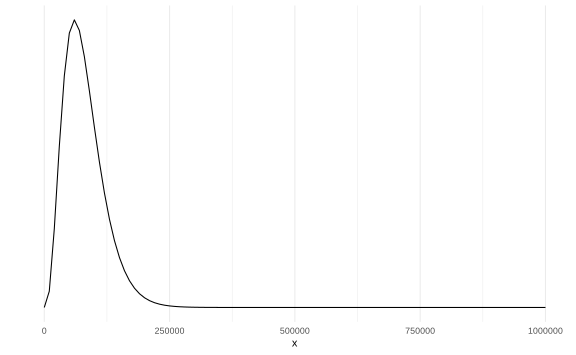
\includegraphics[width=1\linewidth]{Notas-Curso-Estadistica_files/figure-latex/unnamed-chunk-6-1} \end{center}

\hypertarget{distribuciuxf3n-conjunta}{%
\subsection{Distribución conjunta}\label{distribuciuxf3n-conjunta}}

Asumiendo que tenemos algunos datos \(X_1, ..., X_n\), asumimos que estos son exponencial recordando que \(\mathbb E [X] = 1/\theta\), entonces una aproximación de esta densidad es

\begin{Shaded}
\begin{Highlighting}[]
\NormalTok{x \textless{}{-}}\StringTok{ }\KeywordTok{c}\NormalTok{(}\DecValTok{2911}\NormalTok{, }\DecValTok{3403}\NormalTok{, }\DecValTok{3237}\NormalTok{, }\DecValTok{3509}\NormalTok{, }\DecValTok{3118}\NormalTok{)}

\NormalTok{theta \textless{}{-}}\StringTok{ }\DecValTok{1}\OperatorTok{/}\KeywordTok{mean}\NormalTok{(x)}

\KeywordTok{ggplot}\NormalTok{(}\DataTypeTok{data =} \KeywordTok{data.frame}\NormalTok{(}\DataTypeTok{x =} \KeywordTok{c}\NormalTok{(}\DecValTok{0}\NormalTok{, }\FloatTok{1e+05}\NormalTok{)), }\KeywordTok{aes}\NormalTok{(x)) }\OperatorTok{+}\StringTok{ }
\StringTok{    }\KeywordTok{stat\_function}\NormalTok{(}\DataTypeTok{fun =}\NormalTok{ dexp, }\DataTypeTok{args =} \KeywordTok{list}\NormalTok{(}\DataTypeTok{rate =}\NormalTok{ theta)) }\OperatorTok{+}\StringTok{ }
\StringTok{    }\KeywordTok{ylab}\NormalTok{(}\StringTok{""}\NormalTok{) }\OperatorTok{+}\StringTok{ }\KeywordTok{scale\_y\_continuous}\NormalTok{(}\DataTypeTok{breaks =} \OtherTok{NULL}\NormalTok{) }\OperatorTok{+}\StringTok{ }
\StringTok{    }\KeywordTok{theme\_minimal}\NormalTok{()}
\end{Highlighting}
\end{Shaded}

\begin{center}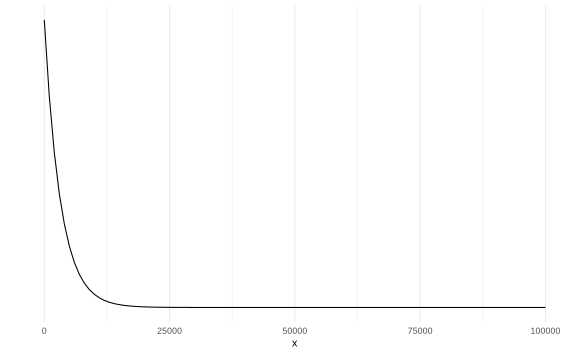
\includegraphics[width=1\linewidth]{Notas-Curso-Estadistica_files/figure-latex/unnamed-chunk-7-1} \end{center}

\hypertarget{distribuciuxf3n-posterior}{%
\subsection{Distribución posterior}\label{distribuciuxf3n-posterior}}

Según los contenidos del curso, se puede estimar los parámetros de la densidad posterior de la forma

\begin{Shaded}
\begin{Highlighting}[]
\NormalTok{(y \textless{}{-}}\StringTok{ }\KeywordTok{sum}\NormalTok{(x))}
\end{Highlighting}
\end{Shaded}

\begin{verbatim}
## [1] 16178
\end{verbatim}

\begin{Shaded}
\begin{Highlighting}[]
\NormalTok{(n \textless{}{-}}\StringTok{ }\KeywordTok{length}\NormalTok{(x))}
\end{Highlighting}
\end{Shaded}

\begin{verbatim}
## [1] 5
\end{verbatim}

\begin{Shaded}
\begin{Highlighting}[]
\NormalTok{(alpha\_posterior \textless{}{-}}\StringTok{ }\NormalTok{n }\OperatorTok{+}\StringTok{ }\NormalTok{alpha\_previa)}
\end{Highlighting}
\end{Shaded}

\begin{verbatim}
## [1] 9
\end{verbatim}

\begin{Shaded}
\begin{Highlighting}[]
\NormalTok{(beta\_posterior \textless{}{-}}\StringTok{ }\NormalTok{beta\_previa }\OperatorTok{+}\StringTok{ }\NormalTok{y)}
\end{Highlighting}
\end{Shaded}

\begin{verbatim}
## [1] 36178
\end{verbatim}

\begin{Shaded}
\begin{Highlighting}[]
\KeywordTok{ggplot}\NormalTok{(}\DataTypeTok{data =} \KeywordTok{data.frame}\NormalTok{(}\DataTypeTok{x =} \KeywordTok{c}\NormalTok{(}\DecValTok{0}\NormalTok{, }\DecValTok{750000}\NormalTok{)), }\KeywordTok{aes}\NormalTok{(x)) }\OperatorTok{+}\StringTok{ }
\StringTok{    }\KeywordTok{stat\_function}\NormalTok{(}\DataTypeTok{fun =}\NormalTok{ dgamma, }\DataTypeTok{args =} \KeywordTok{list}\NormalTok{(}\DataTypeTok{shape =}\NormalTok{ alpha\_previa, }
        \DataTypeTok{scale =}\NormalTok{ beta\_previa), }\KeywordTok{aes}\NormalTok{(}\DataTypeTok{color =} \StringTok{"Previa"}\NormalTok{)) }\OperatorTok{+}\StringTok{ }
\StringTok{    }\KeywordTok{stat\_function}\NormalTok{(}\DataTypeTok{fun =}\NormalTok{ dgamma, }\DataTypeTok{args =} \KeywordTok{list}\NormalTok{(}\DataTypeTok{shape =}\NormalTok{ alpha\_posterior, }
        \DataTypeTok{scale =}\NormalTok{ beta\_posterior), }\KeywordTok{aes}\NormalTok{(}\DataTypeTok{color =} \StringTok{"Posterior"}\NormalTok{)) }\OperatorTok{+}\StringTok{ }
\StringTok{    }\KeywordTok{stat\_function}\NormalTok{(}\DataTypeTok{fun =}\NormalTok{ dexp, }\DataTypeTok{args =} \KeywordTok{list}\NormalTok{(}\DataTypeTok{rate =}\NormalTok{ theta), }
        \KeywordTok{aes}\NormalTok{(}\DataTypeTok{color =} \StringTok{"Verosimilitud"}\NormalTok{)) }\OperatorTok{+}\StringTok{ }\KeywordTok{ylim}\NormalTok{(}\DecValTok{0}\NormalTok{, }\FloatTok{1.5e{-}05}\NormalTok{) }\OperatorTok{+}\StringTok{ }
\StringTok{    }\KeywordTok{theme\_minimal}\NormalTok{()}
\end{Highlighting}
\end{Shaded}

\begin{center}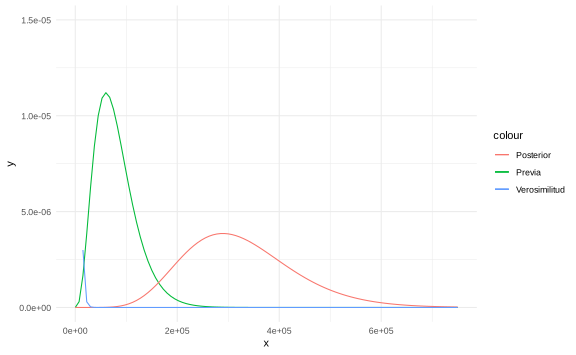
\includegraphics[width=1\linewidth]{Notas-Curso-Estadistica_files/figure-latex/unnamed-chunk-9-1} \end{center}

\hypertarget{agregando-nuevos-datos}{%
\subsection{Agregando nuevos datos}\label{agregando-nuevos-datos}}

Si tenemos un 6to dato, y queremos ver cual es su distribución posterior. Lo primero es estimar la densidad posterior de este 6to dato, pero asumiendo que la previa es la densidad que obtuvimos en el caso anterior.

Suponga que \(X_6 = 3000\)

\begin{Shaded}
\begin{Highlighting}[]
\NormalTok{(alpha\_previa \textless{}{-}}\StringTok{ }\NormalTok{alpha\_posterior)}
\end{Highlighting}
\end{Shaded}

\begin{verbatim}
## [1] 9
\end{verbatim}

\begin{Shaded}
\begin{Highlighting}[]
\NormalTok{(beta\_previa \textless{}{-}}\StringTok{ }\NormalTok{beta\_posterior)}
\end{Highlighting}
\end{Shaded}

\begin{verbatim}
## [1] 36178
\end{verbatim}

\begin{Shaded}
\begin{Highlighting}[]
\NormalTok{(alpha\_posterior \textless{}{-}}\StringTok{ }\NormalTok{alpha\_previa }\OperatorTok{+}\StringTok{ }\DecValTok{1}\NormalTok{)}
\end{Highlighting}
\end{Shaded}

\begin{verbatim}
## [1] 10
\end{verbatim}

\begin{Shaded}
\begin{Highlighting}[]
\NormalTok{(beta\_posterior \textless{}{-}}\StringTok{ }\NormalTok{beta\_previa }\OperatorTok{+}\StringTok{ }\DecValTok{3000}\NormalTok{)}
\end{Highlighting}
\end{Shaded}

\begin{verbatim}
## [1] 39178
\end{verbatim}

\begin{Shaded}
\begin{Highlighting}[]
\KeywordTok{ggplot}\NormalTok{(}\DataTypeTok{data =} \KeywordTok{data.frame}\NormalTok{(}\DataTypeTok{x =} \KeywordTok{c}\NormalTok{(}\DecValTok{0}\NormalTok{, }\FloatTok{1e+06}\NormalTok{)), }\KeywordTok{aes}\NormalTok{(x)) }\OperatorTok{+}\StringTok{ }
\StringTok{    }\KeywordTok{stat\_function}\NormalTok{(}\DataTypeTok{fun =}\NormalTok{ dgamma, }\DataTypeTok{args =} \KeywordTok{list}\NormalTok{(}\DataTypeTok{shape =} \DecValTok{4}\NormalTok{, }
        \DataTypeTok{scale =} \DecValTok{20000}\NormalTok{), }\KeywordTok{aes}\NormalTok{(}\DataTypeTok{color =} \StringTok{"Previa \#1"}\NormalTok{)) }\OperatorTok{+}\StringTok{ }
\StringTok{    }\KeywordTok{stat\_function}\NormalTok{(}\DataTypeTok{fun =}\NormalTok{ dgamma, }\DataTypeTok{args =} \KeywordTok{list}\NormalTok{(}\DataTypeTok{shape =}\NormalTok{ alpha\_previa, }
        \DataTypeTok{scale =}\NormalTok{ beta\_previa), }\KeywordTok{aes}\NormalTok{(}\DataTypeTok{color =} \StringTok{"Previa \#2"}\NormalTok{)) }\OperatorTok{+}\StringTok{ }
\StringTok{    }\KeywordTok{stat\_function}\NormalTok{(}\DataTypeTok{fun =}\NormalTok{ dgamma, }\DataTypeTok{args =} \KeywordTok{list}\NormalTok{(}\DataTypeTok{shape =}\NormalTok{ alpha\_posterior, }
        \DataTypeTok{scale =}\NormalTok{ beta\_posterior), }\KeywordTok{aes}\NormalTok{(}\DataTypeTok{color =} \StringTok{"Posterior"}\NormalTok{)) }\OperatorTok{+}\StringTok{ }
\StringTok{    }\KeywordTok{ylim}\NormalTok{(}\DecValTok{0}\NormalTok{, }\FloatTok{1.5e{-}05}\NormalTok{) }\OperatorTok{+}\StringTok{ }\KeywordTok{theme\_minimal}\NormalTok{()}
\end{Highlighting}
\end{Shaded}

\begin{center}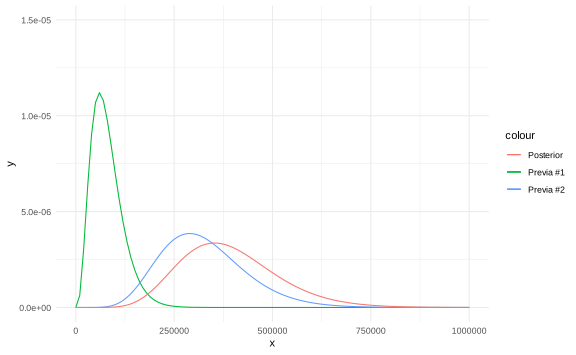
\includegraphics[width=1\linewidth]{Notas-Curso-Estadistica_files/figure-latex/unnamed-chunk-10-1} \end{center}

\hypertarget{familias-conjugadas-normales}{%
\subsection{Familias conjugadas normales}\label{familias-conjugadas-normales}}

Si tenemos pocos datos, la información previa es la que ``prevalece''.

\begin{Shaded}
\begin{Highlighting}[]
\NormalTok{x \textless{}{-}}\StringTok{ }\KeywordTok{rnorm}\NormalTok{(}\DataTypeTok{n =} \DecValTok{3}\NormalTok{, }\DataTypeTok{mean =} \DecValTok{10}\NormalTok{, }\DataTypeTok{sd =} \DecValTok{1}\NormalTok{)}

\NormalTok{(mu \textless{}{-}}\StringTok{ }\KeywordTok{mean}\NormalTok{(x))}
\end{Highlighting}
\end{Shaded}

\begin{verbatim}
## [1] 10.64715
\end{verbatim}

\begin{Shaded}
\begin{Highlighting}[]
\NormalTok{(sigma \textless{}{-}}\StringTok{ }\KeywordTok{sd}\NormalTok{(x))}
\end{Highlighting}
\end{Shaded}

\begin{verbatim}
## [1] 0.5654769
\end{verbatim}

\begin{Shaded}
\begin{Highlighting}[]
\NormalTok{(n \textless{}{-}}\StringTok{ }\KeywordTok{length}\NormalTok{(x))}
\end{Highlighting}
\end{Shaded}

\begin{verbatim}
## [1] 3
\end{verbatim}

\begin{Shaded}
\begin{Highlighting}[]
\NormalTok{(mu\_previa \textless{}{-}}\StringTok{ }\DecValTok{0}\NormalTok{)}
\end{Highlighting}
\end{Shaded}

\begin{verbatim}
## [1] 0
\end{verbatim}

\begin{Shaded}
\begin{Highlighting}[]
\NormalTok{(sigma\_previa \textless{}{-}}\StringTok{ }\DecValTok{1}\NormalTok{)}
\end{Highlighting}
\end{Shaded}

\begin{verbatim}
## [1] 1
\end{verbatim}

\begin{Shaded}
\begin{Highlighting}[]
\NormalTok{(mu\_posterior \textless{}{-}}\StringTok{ }\NormalTok{((sigma}\OperatorTok{\^{}}\DecValTok{2}\NormalTok{)}\OperatorTok{/}\NormalTok{(sigma}\OperatorTok{\^{}}\DecValTok{2} \OperatorTok{+}\StringTok{ }\NormalTok{n }\OperatorTok{*}\StringTok{ }\NormalTok{sigma\_previa}\OperatorTok{\^{}}\DecValTok{2}\NormalTok{)) }\OperatorTok{*}\StringTok{ }
\StringTok{    }\NormalTok{mu\_previa }\OperatorTok{+}\StringTok{ }\NormalTok{((n }\OperatorTok{*}\StringTok{ }\NormalTok{sigma\_previa}\OperatorTok{\^{}}\DecValTok{2}\NormalTok{)}\OperatorTok{/}\NormalTok{(sigma}\OperatorTok{\^{}}\DecValTok{2} \OperatorTok{+}\StringTok{ }\NormalTok{n }\OperatorTok{*}\StringTok{ }
\StringTok{    }\NormalTok{sigma\_previa}\OperatorTok{\^{}}\DecValTok{2}\NormalTok{)) }\OperatorTok{*}\StringTok{ }\NormalTok{mu)}
\end{Highlighting}
\end{Shaded}

\begin{verbatim}
## [1] 9.621605
\end{verbatim}

\begin{Shaded}
\begin{Highlighting}[]
\NormalTok{(sigma2\_posterior \textless{}{-}}\StringTok{ }\NormalTok{(sigma}\OperatorTok{\^{}}\DecValTok{2} \OperatorTok{*}\StringTok{ }\NormalTok{sigma\_previa}\OperatorTok{\^{}}\DecValTok{2}\NormalTok{)}\OperatorTok{/}\NormalTok{(sigma}\OperatorTok{\^{}}\DecValTok{2} \OperatorTok{+}\StringTok{ }
\StringTok{    }\NormalTok{n }\OperatorTok{*}\StringTok{ }\NormalTok{sigma\_previa}\OperatorTok{\^{}}\DecValTok{2}\NormalTok{))}
\end{Highlighting}
\end{Shaded}

\begin{verbatim}
## [1] 0.09632134
\end{verbatim}

\begin{Shaded}
\begin{Highlighting}[]
\KeywordTok{ggplot}\NormalTok{(}\DataTypeTok{data =} \KeywordTok{data.frame}\NormalTok{(}\DataTypeTok{x =} \KeywordTok{c}\NormalTok{(}\OperatorTok{{-}}\DecValTok{5}\NormalTok{, }\DecValTok{15}\NormalTok{)), }\KeywordTok{aes}\NormalTok{(x)) }\OperatorTok{+}\StringTok{ }
\StringTok{    }\KeywordTok{stat\_function}\NormalTok{(}\DataTypeTok{fun =}\NormalTok{ dnorm, }\DataTypeTok{args =} \KeywordTok{list}\NormalTok{(}\DataTypeTok{mean =}\NormalTok{ mu\_previa, }
        \DataTypeTok{sd =}\NormalTok{ sigma\_previa), }\KeywordTok{aes}\NormalTok{(}\DataTypeTok{color =} \StringTok{"Previa"}\NormalTok{)) }\OperatorTok{+}\StringTok{ }
\StringTok{    }\KeywordTok{stat\_function}\NormalTok{(}\DataTypeTok{fun =}\NormalTok{ dnorm, }\DataTypeTok{args =} \KeywordTok{list}\NormalTok{(}\DataTypeTok{mean =}\NormalTok{ mu\_posterior, }
        \DataTypeTok{sd =} \KeywordTok{sqrt}\NormalTok{(sigma2\_posterior)), }\KeywordTok{aes}\NormalTok{(}\DataTypeTok{color =} \StringTok{"Posterior"}\NormalTok{)) }\OperatorTok{+}\StringTok{ }
\StringTok{    }\KeywordTok{stat\_function}\NormalTok{(}\DataTypeTok{fun =}\NormalTok{ dnorm, }\DataTypeTok{args =} \KeywordTok{list}\NormalTok{(}\DataTypeTok{mean =}\NormalTok{ mu, }
        \DataTypeTok{sd =}\NormalTok{ sigma), }\KeywordTok{aes}\NormalTok{(}\DataTypeTok{color =} \StringTok{"Verosimilitud"}\NormalTok{)) }\OperatorTok{+}\StringTok{ }
\StringTok{    }\KeywordTok{theme\_minimal}\NormalTok{()}
\end{Highlighting}
\end{Shaded}

\begin{center}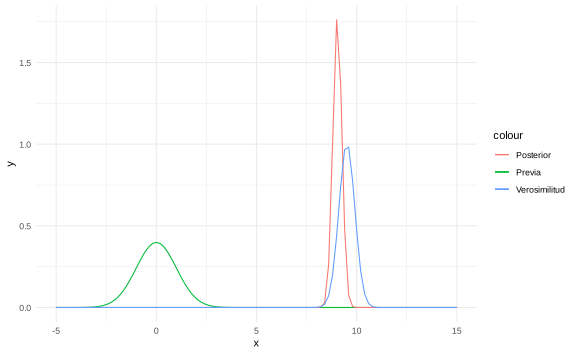
\includegraphics[width=1\linewidth]{Notas-Curso-Estadistica_files/figure-latex/unnamed-chunk-11-1} \end{center}

Con más datos, la distribución se ajusta a esto y le quita importancia a la información previa.

\begin{Shaded}
\begin{Highlighting}[]
\NormalTok{x \textless{}{-}}\StringTok{ }\KeywordTok{rnorm}\NormalTok{(}\DataTypeTok{n =} \DecValTok{100}\NormalTok{, }\DataTypeTok{mean =} \DecValTok{10}\NormalTok{, }\DataTypeTok{sd =} \DecValTok{1}\NormalTok{)}

\NormalTok{(mu \textless{}{-}}\StringTok{ }\KeywordTok{mean}\NormalTok{(x))}
\end{Highlighting}
\end{Shaded}

\begin{verbatim}
## [1] 9.994564
\end{verbatim}

\begin{Shaded}
\begin{Highlighting}[]
\NormalTok{(sigma \textless{}{-}}\StringTok{ }\KeywordTok{sd}\NormalTok{(x))}
\end{Highlighting}
\end{Shaded}

\begin{verbatim}
## [1] 1.060066
\end{verbatim}

\begin{Shaded}
\begin{Highlighting}[]
\NormalTok{(n \textless{}{-}}\StringTok{ }\KeywordTok{length}\NormalTok{(x))}
\end{Highlighting}
\end{Shaded}

\begin{verbatim}
## [1] 100
\end{verbatim}

\begin{Shaded}
\begin{Highlighting}[]
\NormalTok{(mu\_previa \textless{}{-}}\StringTok{ }\DecValTok{0}\NormalTok{)}
\end{Highlighting}
\end{Shaded}

\begin{verbatim}
## [1] 0
\end{verbatim}

\begin{Shaded}
\begin{Highlighting}[]
\NormalTok{(sigma\_previa \textless{}{-}}\StringTok{ }\DecValTok{1}\NormalTok{)}
\end{Highlighting}
\end{Shaded}

\begin{verbatim}
## [1] 1
\end{verbatim}

\begin{Shaded}
\begin{Highlighting}[]
\NormalTok{(mu\_posterior \textless{}{-}}\StringTok{ }\NormalTok{((sigma}\OperatorTok{\^{}}\DecValTok{2}\NormalTok{)}\OperatorTok{/}\NormalTok{(sigma}\OperatorTok{\^{}}\DecValTok{2} \OperatorTok{+}\StringTok{ }\NormalTok{n }\OperatorTok{*}\StringTok{ }\NormalTok{sigma\_previa}\OperatorTok{\^{}}\DecValTok{2}\NormalTok{)) }\OperatorTok{*}\StringTok{ }
\StringTok{    }\NormalTok{mu\_previa }\OperatorTok{+}\StringTok{ }\NormalTok{((n }\OperatorTok{*}\StringTok{ }\NormalTok{sigma\_previa}\OperatorTok{\^{}}\DecValTok{2}\NormalTok{)}\OperatorTok{/}\NormalTok{(sigma}\OperatorTok{\^{}}\DecValTok{2} \OperatorTok{+}\StringTok{ }\NormalTok{n }\OperatorTok{*}\StringTok{ }
\StringTok{    }\NormalTok{sigma\_previa}\OperatorTok{\^{}}\DecValTok{2}\NormalTok{)) }\OperatorTok{*}\StringTok{ }\NormalTok{mu)}
\end{Highlighting}
\end{Shaded}

\begin{verbatim}
## [1] 9.883499
\end{verbatim}

\begin{Shaded}
\begin{Highlighting}[]
\NormalTok{(sigma2\_posterior \textless{}{-}}\StringTok{ }\NormalTok{(sigma}\OperatorTok{\^{}}\DecValTok{2} \OperatorTok{*}\StringTok{ }\NormalTok{sigma\_previa}\OperatorTok{\^{}}\DecValTok{2}\NormalTok{)}\OperatorTok{/}\NormalTok{(sigma}\OperatorTok{\^{}}\DecValTok{2} \OperatorTok{+}\StringTok{ }
\StringTok{    }\NormalTok{n }\OperatorTok{*}\StringTok{ }\NormalTok{sigma\_previa}\OperatorTok{\^{}}\DecValTok{2}\NormalTok{))}
\end{Highlighting}
\end{Shaded}

\begin{verbatim}
## [1] 0.01111253
\end{verbatim}

\begin{Shaded}
\begin{Highlighting}[]
\KeywordTok{ggplot}\NormalTok{(}\DataTypeTok{data =} \KeywordTok{data.frame}\NormalTok{(}\DataTypeTok{x =} \KeywordTok{c}\NormalTok{(}\OperatorTok{{-}}\DecValTok{5}\NormalTok{, }\DecValTok{15}\NormalTok{)), }\KeywordTok{aes}\NormalTok{(x)) }\OperatorTok{+}\StringTok{ }
\StringTok{    }\KeywordTok{stat\_function}\NormalTok{(}\DataTypeTok{fun =}\NormalTok{ dnorm, }\DataTypeTok{args =} \KeywordTok{list}\NormalTok{(}\DataTypeTok{mean =}\NormalTok{ mu\_previa, }
        \DataTypeTok{sd =}\NormalTok{ sigma\_previa), }\KeywordTok{aes}\NormalTok{(}\DataTypeTok{color =} \StringTok{"Previa"}\NormalTok{)) }\OperatorTok{+}\StringTok{ }
\StringTok{    }\KeywordTok{stat\_function}\NormalTok{(}\DataTypeTok{fun =}\NormalTok{ dnorm, }\DataTypeTok{args =} \KeywordTok{list}\NormalTok{(}\DataTypeTok{mean =}\NormalTok{ mu\_posterior, }
        \DataTypeTok{sd =} \KeywordTok{sqrt}\NormalTok{(sigma2\_posterior)), }\KeywordTok{aes}\NormalTok{(}\DataTypeTok{color =} \StringTok{"Posterior"}\NormalTok{)) }\OperatorTok{+}\StringTok{ }
\StringTok{    }\KeywordTok{stat\_function}\NormalTok{(}\DataTypeTok{fun =}\NormalTok{ dnorm, }\DataTypeTok{args =} \KeywordTok{list}\NormalTok{(}\DataTypeTok{mean =}\NormalTok{ mu, }
        \DataTypeTok{sd =}\NormalTok{ sigma), }\KeywordTok{aes}\NormalTok{(}\DataTypeTok{color =} \StringTok{"Verosimilitud"}\NormalTok{)) }\OperatorTok{+}\StringTok{ }
\StringTok{    }\KeywordTok{theme\_minimal}\NormalTok{()}
\end{Highlighting}
\end{Shaded}

\begin{center}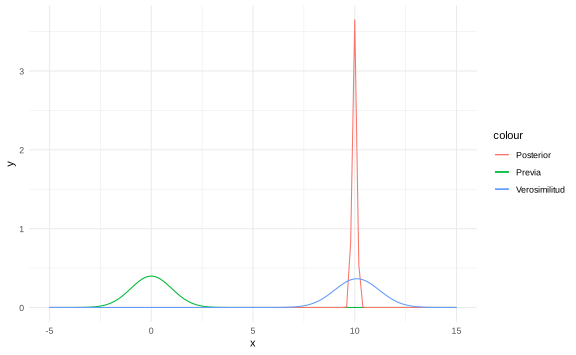
\includegraphics[width=1\linewidth]{Notas-Curso-Estadistica_files/figure-latex/unnamed-chunk-12-1} \end{center}

Si los datos por si solo son muy variable, la posterior tiende a parecerse a la
distribución previa en lugar que a la verosimilitud.

\begin{Shaded}
\begin{Highlighting}[]
\NormalTok{x \textless{}{-}}\StringTok{ }\KeywordTok{rnorm}\NormalTok{(}\DataTypeTok{n =} \DecValTok{10}\NormalTok{, }\DataTypeTok{mean =} \DecValTok{10}\NormalTok{, }\DataTypeTok{sd =} \DecValTok{5}\NormalTok{)}

\NormalTok{(mu \textless{}{-}}\StringTok{ }\KeywordTok{mean}\NormalTok{(x))}
\end{Highlighting}
\end{Shaded}

\begin{verbatim}
## [1] 9.576984
\end{verbatim}

\begin{Shaded}
\begin{Highlighting}[]
\NormalTok{(sigma \textless{}{-}}\StringTok{ }\KeywordTok{sd}\NormalTok{(x))}
\end{Highlighting}
\end{Shaded}

\begin{verbatim}
## [1] 7.32444
\end{verbatim}

\begin{Shaded}
\begin{Highlighting}[]
\NormalTok{(n \textless{}{-}}\StringTok{ }\KeywordTok{length}\NormalTok{(x))}
\end{Highlighting}
\end{Shaded}

\begin{verbatim}
## [1] 10
\end{verbatim}

\begin{Shaded}
\begin{Highlighting}[]
\NormalTok{(mu\_previa \textless{}{-}}\StringTok{ }\DecValTok{0}\NormalTok{)}
\end{Highlighting}
\end{Shaded}

\begin{verbatim}
## [1] 0
\end{verbatim}

\begin{Shaded}
\begin{Highlighting}[]
\NormalTok{(sigma\_previa \textless{}{-}}\StringTok{ }\DecValTok{1}\NormalTok{)}
\end{Highlighting}
\end{Shaded}

\begin{verbatim}
## [1] 1
\end{verbatim}

\begin{Shaded}
\begin{Highlighting}[]
\NormalTok{(mu\_posterior \textless{}{-}}\StringTok{ }\NormalTok{((sigma}\OperatorTok{\^{}}\DecValTok{2}\NormalTok{)}\OperatorTok{/}\NormalTok{(sigma}\OperatorTok{\^{}}\DecValTok{2} \OperatorTok{+}\StringTok{ }\NormalTok{n }\OperatorTok{*}\StringTok{ }\NormalTok{sigma\_previa}\OperatorTok{\^{}}\DecValTok{2}\NormalTok{)) }\OperatorTok{*}\StringTok{ }
\StringTok{    }\NormalTok{mu\_previa }\OperatorTok{+}\StringTok{ }\NormalTok{((n }\OperatorTok{*}\StringTok{ }\NormalTok{sigma\_previa}\OperatorTok{\^{}}\DecValTok{2}\NormalTok{)}\OperatorTok{/}\NormalTok{(sigma}\OperatorTok{\^{}}\DecValTok{2} \OperatorTok{+}\StringTok{ }\NormalTok{n }\OperatorTok{*}\StringTok{ }
\StringTok{    }\NormalTok{sigma\_previa}\OperatorTok{\^{}}\DecValTok{2}\NormalTok{)) }\OperatorTok{*}\StringTok{ }\NormalTok{mu)}
\end{Highlighting}
\end{Shaded}

\begin{verbatim}
## [1] 1.504693
\end{verbatim}

\begin{Shaded}
\begin{Highlighting}[]
\NormalTok{(sigma2\_posterior \textless{}{-}}\StringTok{ }\NormalTok{(sigma}\OperatorTok{\^{}}\DecValTok{2} \OperatorTok{*}\StringTok{ }\NormalTok{sigma\_previa}\OperatorTok{\^{}}\DecValTok{2}\NormalTok{)}\OperatorTok{/}\NormalTok{(sigma}\OperatorTok{\^{}}\DecValTok{2} \OperatorTok{+}\StringTok{ }
\StringTok{    }\NormalTok{n }\OperatorTok{*}\StringTok{ }\NormalTok{sigma\_previa}\OperatorTok{\^{}}\DecValTok{2}\NormalTok{))}
\end{Highlighting}
\end{Shaded}

\begin{verbatim}
## [1] 0.8428844
\end{verbatim}

\begin{Shaded}
\begin{Highlighting}[]
\KeywordTok{ggplot}\NormalTok{(}\DataTypeTok{data =} \KeywordTok{data.frame}\NormalTok{(}\DataTypeTok{x =} \KeywordTok{c}\NormalTok{(}\OperatorTok{{-}}\DecValTok{5}\NormalTok{, }\DecValTok{15}\NormalTok{)), }\KeywordTok{aes}\NormalTok{(x)) }\OperatorTok{+}\StringTok{ }
\StringTok{    }\KeywordTok{stat\_function}\NormalTok{(}\DataTypeTok{fun =}\NormalTok{ dnorm, }\DataTypeTok{args =} \KeywordTok{list}\NormalTok{(}\DataTypeTok{mean =}\NormalTok{ mu\_previa, }
        \DataTypeTok{sd =}\NormalTok{ sigma\_previa), }\KeywordTok{aes}\NormalTok{(}\DataTypeTok{color =} \StringTok{"Previa"}\NormalTok{)) }\OperatorTok{+}\StringTok{ }
\StringTok{    }\KeywordTok{stat\_function}\NormalTok{(}\DataTypeTok{fun =}\NormalTok{ dnorm, }\DataTypeTok{args =} \KeywordTok{list}\NormalTok{(}\DataTypeTok{mean =}\NormalTok{ mu\_posterior, }
        \DataTypeTok{sd =} \KeywordTok{sqrt}\NormalTok{(sigma2\_posterior)), }\KeywordTok{aes}\NormalTok{(}\DataTypeTok{color =} \StringTok{"Posterior"}\NormalTok{)) }\OperatorTok{+}\StringTok{ }
\StringTok{    }\KeywordTok{stat\_function}\NormalTok{(}\DataTypeTok{fun =}\NormalTok{ dnorm, }\DataTypeTok{args =} \KeywordTok{list}\NormalTok{(}\DataTypeTok{mean =}\NormalTok{ mu, }
        \DataTypeTok{sd =}\NormalTok{ sigma), }\KeywordTok{aes}\NormalTok{(}\DataTypeTok{color =} \StringTok{"Verosimilitud"}\NormalTok{)) }\OperatorTok{+}\StringTok{ }
\StringTok{    }\KeywordTok{theme\_minimal}\NormalTok{()}
\end{Highlighting}
\end{Shaded}

\begin{center}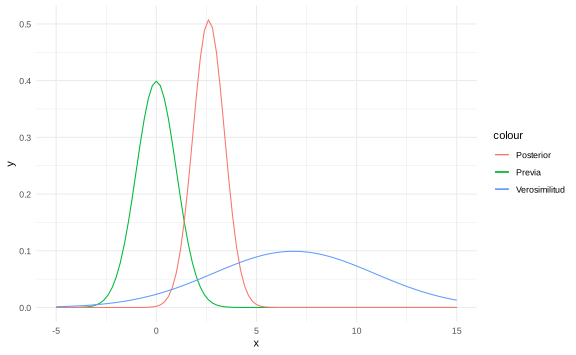
\includegraphics[width=1\linewidth]{Notas-Curso-Estadistica_files/figure-latex/unnamed-chunk-13-1} \end{center}

\hypertarget{funciones-de-puxe9rdida-1}{%
\subsection{Funciones de pérdida}\label{funciones-de-puxe9rdida-1}}

Lo más importante acá es que dependiendo de la función de pérdida podemos construir una estimador para \(\theta\). En el caso de los componentes electrónicos recordemos que la posterior nos daba

\begin{Shaded}
\begin{Highlighting}[]
\NormalTok{alpha \textless{}{-}}\StringTok{ }\DecValTok{9}
\NormalTok{beta \textless{}{-}}\StringTok{ }\DecValTok{36178}
\end{Highlighting}
\end{Shaded}

\begin{itemize}
\tightlist
\item
  \textbf{Pérdida cuadrática:} Recoremos que la media de una gamma es \(\alpha/\beta\) entonces
\end{itemize}

\begin{Shaded}
\begin{Highlighting}[]
\NormalTok{(theta \textless{}{-}}\StringTok{ }\NormalTok{alpha}\OperatorTok{/}\NormalTok{beta)}
\end{Highlighting}
\end{Shaded}

\begin{verbatim}
## [1] 0.00024877
\end{verbatim}

Y por lo tanto el tiempo promedio del componente electrónico es \(1/\theta\)=4019.7777778.

\begin{itemize}
\tightlist
\item
  \textbf{Pérdidad absoluta:} La distribución Gamma no tiene una forma cerrada para la mediana, por que se puede aproximar así,
\end{itemize}

\begin{Shaded}
\begin{Highlighting}[]
\NormalTok{m \textless{}{-}}\StringTok{ }\KeywordTok{rgamma}\NormalTok{(}\DataTypeTok{n =} \DecValTok{1000}\NormalTok{, }\DataTypeTok{scale =}\NormalTok{ beta, }\DataTypeTok{shape =}\NormalTok{ alpha)}
\NormalTok{(theta \textless{}{-}}\StringTok{ }\KeywordTok{median}\NormalTok{(m))}
\end{Highlighting}
\end{Shaded}

\begin{verbatim}
## [1] 312498.7
\end{verbatim}

Y por lo tanto el tiempo promedio del componente electrónico es \(1/\theta\)=\ensuremath{3.2000131\times 10^{-6}}.

\textbf{OJO: En este caso la pérdida cuadrática ajusta mejor ya que la distribución que la pérdida absoluta ya que la distribución NO es simétrica. En el caso simétrico los resultados serían muy similares.}

\hypertarget{caso-concreto}{%
\subsection{Caso concreto}\label{caso-concreto}}

Suponga que se que quiere averiguar si los estudiantes de cierto colegio duermen más de 8 horas o menos de 8 horas.

Para esto primero cargaremos el siguiente paquete,

\begin{Shaded}
\begin{Highlighting}[]
\KeywordTok{library}\NormalTok{(LearnBayes)}
\end{Highlighting}
\end{Shaded}

Suponga que se hace una encuesta a 27 estudiantes y se encuentra que 11 dicen que duermen más de 8 horas diarias y el resto no. Nuestro objetivo es encontrar inferencias sobre la proporción \(p\) de estudiantes que duermen al menos 8 horas diarias. El modelo más adecuado es

\[
f(x \vert p) \propto p^s (1-p)^f
\]

donde \(s\) es la cantidad de estudiantes que duermen más de 8 horas y \(f\) los que duermen menos de 8 horas.

Una primera aproximación para la previa es usar una distribución discreta. En este caso, el investigador asigna una probabilidad a cierta cantidad de horas de sueño, según su experiencia. Así, por ejemplo:

\begin{Shaded}
\begin{Highlighting}[]
\NormalTok{p \textless{}{-}}\StringTok{ }\KeywordTok{seq}\NormalTok{(}\FloatTok{0.05}\NormalTok{, }\FloatTok{0.95}\NormalTok{, }\DataTypeTok{by =} \FloatTok{0.1}\NormalTok{)}
\NormalTok{prior \textless{}{-}}\StringTok{ }\KeywordTok{c}\NormalTok{(}\DecValTok{1}\NormalTok{, }\FloatTok{5.2}\NormalTok{, }\DecValTok{8}\NormalTok{, }\FloatTok{7.2}\NormalTok{, }\FloatTok{4.6}\NormalTok{, }\FloatTok{2.1}\NormalTok{, }\FloatTok{0.7}\NormalTok{, }\FloatTok{0.1}\NormalTok{, }\DecValTok{0}\NormalTok{, }\DecValTok{0}\NormalTok{)}
\NormalTok{prior \textless{}{-}}\StringTok{ }\NormalTok{prior}\OperatorTok{/}\KeywordTok{sum}\NormalTok{(prior)}
\KeywordTok{plot}\NormalTok{(p, prior, }\DataTypeTok{type =} \StringTok{"h"}\NormalTok{, }\DataTypeTok{ylab =} \StringTok{"Probabilidad Previa"}\NormalTok{)}
\end{Highlighting}
\end{Shaded}

\begin{center}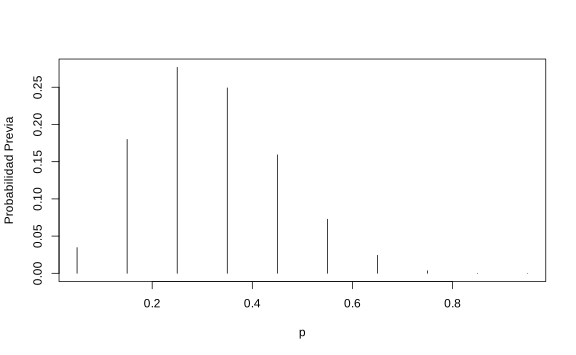
\includegraphics[width=1\linewidth]{Notas-Curso-Estadistica_files/figure-latex/unnamed-chunk-18-1} \end{center}

El paquete \texttt{LearnBayes} tiene la función \texttt{pdisc} que estima la distribución posterior para una previa discreta binomial. Recuerde que el valor 11 representa la cantidad de estudiantes con más de 8 horas de sueño y 16 lo que no duermen esa cantidad.

\begin{Shaded}
\begin{Highlighting}[]
\NormalTok{data \textless{}{-}}\StringTok{ }\KeywordTok{c}\NormalTok{(}\DecValTok{11}\NormalTok{, }\DecValTok{16}\NormalTok{)}
\NormalTok{post \textless{}{-}}\StringTok{ }\KeywordTok{pdisc}\NormalTok{(p, prior, data)}
\KeywordTok{round}\NormalTok{(}\KeywordTok{cbind}\NormalTok{(p, prior, post), }\DecValTok{2}\NormalTok{)}
\end{Highlighting}
\end{Shaded}

\begin{verbatim}
##          p prior post
##  [1,] 0.05  0.03 0.00
##  [2,] 0.15  0.18 0.00
##  [3,] 0.25  0.28 0.13
##  [4,] 0.35  0.25 0.48
##  [5,] 0.45  0.16 0.33
##  [6,] 0.55  0.07 0.06
##  [7,] 0.65  0.02 0.00
##  [8,] 0.75  0.00 0.00
##  [9,] 0.85  0.00 0.00
## [10,] 0.95  0.00 0.00
\end{verbatim}

Y podemos ver la diferencia entre la previa (negro) y la posterior (roja),

\begin{Shaded}
\begin{Highlighting}[]
\KeywordTok{plot}\NormalTok{(p, post, }\DataTypeTok{type =} \StringTok{"h"}\NormalTok{, }\DataTypeTok{col =} \StringTok{"red"}\NormalTok{)}
\KeywordTok{lines}\NormalTok{(p }\OperatorTok{+}\StringTok{ }\FloatTok{0.01}\NormalTok{, prior, }\DataTypeTok{type =} \StringTok{"h"}\NormalTok{)}
\end{Highlighting}
\end{Shaded}

\begin{center}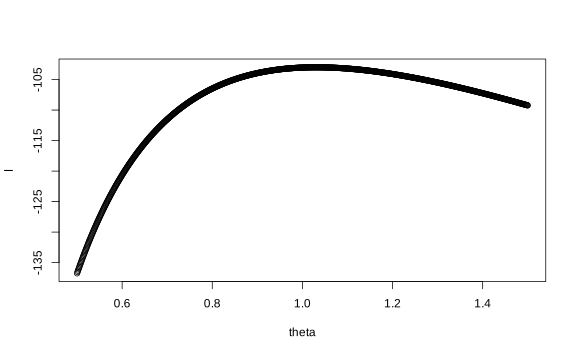
\includegraphics[width=1\linewidth]{Notas-Curso-Estadistica_files/figure-latex/unnamed-chunk-20-1} \end{center}

¿Qué se puede deducir de estos resultados?

\textbf{Ejercicio:} Suponga que se tiene la base de datos \texttt{studentdata}. Realice los cálculos anteriores con esos datos,

\begin{Shaded}
\begin{Highlighting}[]
\KeywordTok{data}\NormalTok{(}\StringTok{"studentdata"}\NormalTok{)}
\NormalTok{horas\_sueno \textless{}{-}}\StringTok{ }\NormalTok{studentdata}\OperatorTok{$}\NormalTok{WakeUp }\OperatorTok{{-}}\StringTok{ }\NormalTok{studentdata}\OperatorTok{$}\NormalTok{ToSleep}
\NormalTok{horas\_sueno \textless{}{-}}\StringTok{ }\KeywordTok{na.omit}\NormalTok{(horas\_sueno)}
\KeywordTok{summary}\NormalTok{(horas\_sueno)}
\end{Highlighting}
\end{Shaded}

\begin{verbatim}
##    Min. 1st Qu.  Median    Mean 3rd Qu.    Max. 
##   2.500   6.500   7.500   7.385   8.500  12.500
\end{verbatim}

\begin{Shaded}
\begin{Highlighting}[]
\KeywordTok{hist}\NormalTok{(horas\_sueno, }\DataTypeTok{main =} \StringTok{""}\NormalTok{)}
\end{Highlighting}
\end{Shaded}

\begin{center}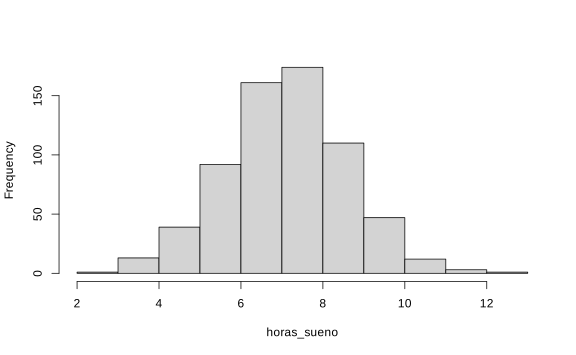
\includegraphics[width=1\linewidth]{Notas-Curso-Estadistica_files/figure-latex/unnamed-chunk-21-1} \end{center}

Ahora supongamos que se tiene quiere ajustar una previa continua a este modelo. Para esto usaremos una distribución Beta con parámetros \(\alpha\) y \(\beta\), de la forma

\[
pi(p\vert \alpha, \beta) \propto p^{1-\alpha} (1-p)^{1-\beta}.
\]

El ajuste de los paramétros de la Beta depende mucho de la información previa que se tenga del modelo. Una forma fácil de estimarlo es a través de cuantiles con los cuales se puede reescribir estos parámetros. Para una explicación detallada revisar \url{https://stats.stackexchange.com/a/237849}

En particular, suponga que se cree que el \(50\%\) de las observaciones la proporción será menor que 0.3 y que el \(90\%\) será menor que 0.5.

Para esto ajustaremos los siguientes parámetros

\begin{Shaded}
\begin{Highlighting}[]
\NormalTok{quantile2 \textless{}{-}}\StringTok{ }\KeywordTok{list}\NormalTok{(}\DataTypeTok{p =} \FloatTok{0.9}\NormalTok{, }\DataTypeTok{x =} \FloatTok{0.5}\NormalTok{)}
\NormalTok{quantile1 \textless{}{-}}\StringTok{ }\KeywordTok{list}\NormalTok{(}\DataTypeTok{p =} \FloatTok{0.5}\NormalTok{, }\DataTypeTok{x =} \FloatTok{0.3}\NormalTok{)}
\NormalTok{(ab \textless{}{-}}\StringTok{ }\KeywordTok{beta.select}\NormalTok{(quantile1, quantile2))}
\end{Highlighting}
\end{Shaded}

\begin{verbatim}
## [1] 3.26 7.19
\end{verbatim}

\begin{Shaded}
\begin{Highlighting}[]
\NormalTok{a \textless{}{-}}\StringTok{ }\NormalTok{ab[}\DecValTok{1}\NormalTok{]}
\NormalTok{b \textless{}{-}}\StringTok{ }\NormalTok{ab[}\DecValTok{2}\NormalTok{]}
\NormalTok{s \textless{}{-}}\StringTok{ }\DecValTok{11}
\NormalTok{f \textless{}{-}}\StringTok{ }\DecValTok{16}
\end{Highlighting}
\end{Shaded}

En este caso se obtendra la distribución posterior Beta con paramétros \(\alpha + s\) y \(\beta + f\),

\begin{Shaded}
\begin{Highlighting}[]
\KeywordTok{curve}\NormalTok{(}\KeywordTok{dbeta}\NormalTok{(x, a }\OperatorTok{+}\StringTok{ }\NormalTok{s, b }\OperatorTok{+}\StringTok{ }\NormalTok{f), }\DataTypeTok{from =} \DecValTok{0}\NormalTok{, }\DataTypeTok{to =} \DecValTok{1}\NormalTok{, }\DataTypeTok{xlab =} \StringTok{"p"}\NormalTok{, }
    \DataTypeTok{ylab =} \StringTok{"Densidad"}\NormalTok{, }\DataTypeTok{lty =} \DecValTok{1}\NormalTok{, }\DataTypeTok{lwd =} \DecValTok{4}\NormalTok{)}
\KeywordTok{curve}\NormalTok{(}\KeywordTok{dbeta}\NormalTok{(x, s }\OperatorTok{+}\StringTok{ }\DecValTok{1}\NormalTok{, f }\OperatorTok{+}\StringTok{ }\DecValTok{1}\NormalTok{), }\DataTypeTok{add =} \OtherTok{TRUE}\NormalTok{, }\DataTypeTok{lty =} \DecValTok{2}\NormalTok{, }
    \DataTypeTok{lwd =} \DecValTok{4}\NormalTok{)}
\KeywordTok{curve}\NormalTok{(}\KeywordTok{dbeta}\NormalTok{(x, a, b), }\DataTypeTok{add =} \OtherTok{TRUE}\NormalTok{, }\DataTypeTok{lty =} \DecValTok{3}\NormalTok{, }\DataTypeTok{lwd =} \DecValTok{4}\NormalTok{)}
\KeywordTok{legend}\NormalTok{(}\FloatTok{0.7}\NormalTok{, }\DecValTok{4}\NormalTok{, }\KeywordTok{c}\NormalTok{(}\StringTok{"Previa"}\NormalTok{, }\StringTok{"Verosimilitud"}\NormalTok{, }\StringTok{"Posterior"}\NormalTok{), }
    \DataTypeTok{lty =} \KeywordTok{c}\NormalTok{(}\DecValTok{3}\NormalTok{, }\DecValTok{2}\NormalTok{, }\DecValTok{1}\NormalTok{), }\DataTypeTok{lwd =} \KeywordTok{c}\NormalTok{(}\DecValTok{3}\NormalTok{, }\DecValTok{3}\NormalTok{, }\DecValTok{3}\NormalTok{))}
\end{Highlighting}
\end{Shaded}

\begin{center}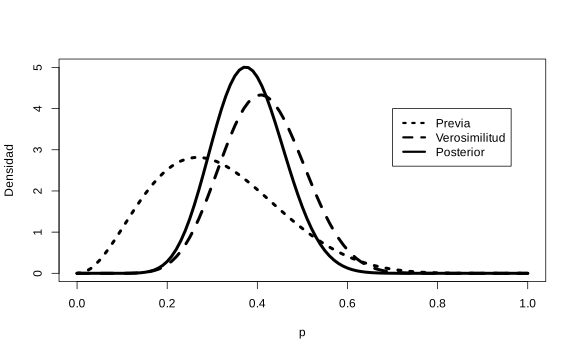
\includegraphics[width=1\linewidth]{Notas-Curso-Estadistica_files/figure-latex/unnamed-chunk-23-1} \end{center}

\hypertarget{estimaciuxf3n-por-muxe1xima-verosimilitud}{%
\chapter{Estimación por máxima verosimilitud}\label{estimaciuxf3n-por-muxe1xima-verosimilitud}}

¿Será posible estimar sin una densidad previa? Se debería ajustar la noción de
muestra a independencia dado el valor de un parámetro.

Recuerde que, para \(X_1,\dots, X_n \stackrel{i.i.d}{\sim} f(X|\theta)\) con \(\theta\)
fijo, la \textbf{función de verosimilitud} se define como \[ f_n(X|\theta) =
\pi(X_i|\theta) = G(\theta|X).\]

Si \(\theta_1,\theta_2\in \Omega\), \(\theta\) es el valor real del parámetro. Si la muestra es
fija, evaluamos, para \(\theta_1\), \(f_n(X|\theta_1) = L(\theta_1|X)\) y, de igual forma para
\(\theta_2\), \(f_n(X|\theta_2) = L(\theta_2|X)\). Supongamos que

\begin{equation*}
f_n(X|\theta_1) >f_n(X|\theta_2) \implies L(\theta_1|X)>L(\theta_2|X) \text{
(principio de verosimilitud)} 
\end{equation*}

\textbf{Interpretación}. Es más verosímil (realista) que el verdadero parámetro sea
\(\theta_1\) que \(\theta_2\) dada la muestra.

\textbf{Definición}. Para cada \(x\in \mathcal{X}\) (espacio muestral), sea
\(\delta(x) \in \delta\) estimador de \(\theta\) tal que \(f_n(x|\theta)\) es máximo. A
\(\delta(x)\) se le llama \textbf{MLE (estimador de máxima verosimilitud)}.

\textbf{Ejemplo}. Si \(X_1,\dots, X_n \sim \text{Exp}(\theta)\), estime \(\theta\).

Determinamos la función de verosimilitud,

\begin{equation*} 
f_n(X|\theta) =
\prod_{i=1}^n \dfrac{1}\theta e^{-X_i/\theta} = \dfrac1{\theta^n}
\exp\left(\dfrac{1}\theta \sum_{i=1}^nX_i\right) = \theta^{-n}e^{-y/\theta}.
\end{equation*}

Considere la \textbf{log-verosimilitud}
\begin{equation*}
\ell(\theta|X) = \ln f_n(X|\theta) = -n\ln \theta - \dfrac{y}{\theta}
\end{equation*}

Como es una transformación monótona creciente, la función de verosimilitud se
maximiza si la log-verosimilitud es máxima. Entonces,

\begin{align*}
\dfrac{\partial}{\partial\theta} \ell(\theta|X) & = \dfrac{-n}{\theta}+\dfrac{y}{\theta^2} = 0 \\
\implies \dfrac{1}{\theta}\left(-n+\dfrac{y}\theta\right) & =0  \\
\implies \hat\theta = \dfrac{y}{n} & = \bar X_n.
\end{align*}

Para verificar que es un máximo:

\[\dfrac{\partial^2    \ell}{\partial\theta^2} = \left. \dfrac{n}{\theta^2} -\dfrac{2y}{\theta^3}\right\vert_{\theta = \frac{y}{n}} = \dfrac{1}{\hat\theta^2} \bigg[n-\dfrac{2y}{\frac yn}\bigg] = \dfrac{-n}{\hat\theta^2} < 0.\]

Entonces \(\hat\theta = \bar X_n\) es el MLE de \(\theta\).

\textbf{Laboratorio:}

Suponga que se tiene 100 valores con distribución exponencial con parámetro
\(\theta=1\).

\begin{Shaded}
\begin{Highlighting}[]
\NormalTok{x \textless{}{-}}\StringTok{ }\KeywordTok{rexp}\NormalTok{(}\DataTypeTok{n =} \DecValTok{100}\NormalTok{, }\DataTypeTok{rate =} \DecValTok{1}\NormalTok{)}
\NormalTok{n \textless{}{-}}\StringTok{ }\KeywordTok{length}\NormalTok{(x)}
\NormalTok{y \textless{}{-}}\StringTok{ }\KeywordTok{sum}\NormalTok{(x)}
\NormalTok{theta \textless{}{-}}\StringTok{ }\KeywordTok{seq}\NormalTok{(}\FloatTok{0.5}\NormalTok{, }\FloatTok{1.5}\NormalTok{, }\DataTypeTok{length.out =} \DecValTok{1000}\NormalTok{)}
\end{Highlighting}
\end{Shaded}

\begin{Shaded}
\begin{Highlighting}[]
\NormalTok{L \textless{}{-}}\StringTok{ }\NormalTok{theta}\OperatorTok{\^{}}\NormalTok{(}\OperatorTok{{-}}\NormalTok{n) }\OperatorTok{*}\StringTok{ }\KeywordTok{exp}\NormalTok{(}\OperatorTok{{-}}\NormalTok{y}\OperatorTok{/}\NormalTok{theta)}
\KeywordTok{plot}\NormalTok{(theta, L)}
\end{Highlighting}
\end{Shaded}

\begin{center}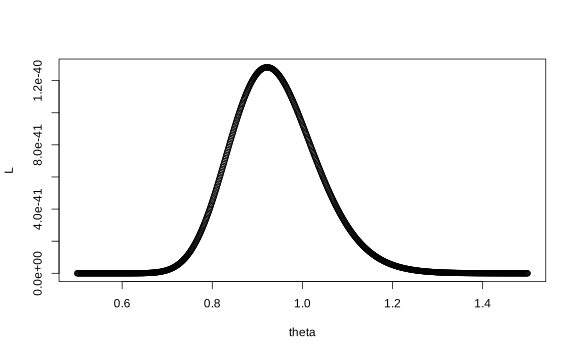
\includegraphics[width=1\linewidth]{Notas-Curso-Estadistica_files/figure-latex/unnamed-chunk-26-1} \end{center}

\begin{Shaded}
\begin{Highlighting}[]
\NormalTok{l \textless{}{-}}\StringTok{ }\OperatorTok{{-}}\NormalTok{n }\OperatorTok{*}\StringTok{ }\KeywordTok{log}\NormalTok{(theta) }\OperatorTok{{-}}\StringTok{ }\NormalTok{y}\OperatorTok{/}\NormalTok{theta}
\KeywordTok{plot}\NormalTok{(theta, l)}
\end{Highlighting}
\end{Shaded}

\begin{center}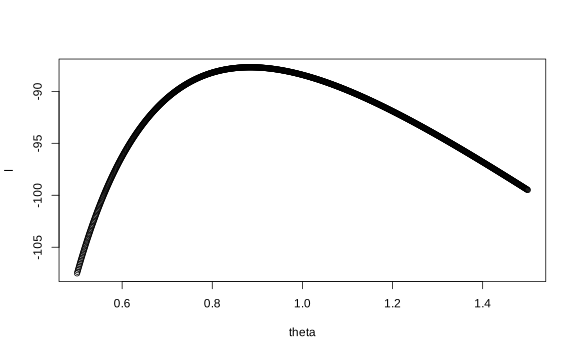
\includegraphics[width=1\linewidth]{Notas-Curso-Estadistica_files/figure-latex/unnamed-chunk-27-1} \end{center}

\textbf{Ejemplo}. En una prueba sobre alguna enfermedad, en un \(90\%\) da la verdadera condición (enfermo) y en un \(10\%\) la prueba se equivoca (que diga que la persona esté enferma cuando está sana). Considere una variable aleatoria \(\text{Bernoulli}(\theta)\),\(\theta \in \{0.9,0.1\}\)
Una muestra sería
\[x = \begin{cases}1 & \text{si la prueba es positiva}\\0& \text{si no}\end{cases}\]
Si \(x=0\), entonces \(f(0|\theta) = \begin{cases}0.9 & \text{si }\theta = 0.1\\0.1& \text{si }\theta = 0.9\end{cases}\).

Si \(x=1\), entonces \(f(1|\theta) = \begin{cases}0.1 & \text{si }\theta = 0.1\\0.9& \text{si }\theta = 0.9\end{cases}\).

El MLE corresponde a
\[\hat\theta = \begin{cases}0.1 & \text{si }x= 0\\0.9& \text{si }x= 1\end{cases}\]

\textbf{Ejemplo}. Para el caso normal, \(X_1,\dots, X_n \sim N(\mu,\sigma^2)\), \(\sigma^2\) conocida, estime \(\mu\).

\[f_n(x|\mu) = \prod_{i=1}^n \dfrac{1}{\sqrt{2\pi\sigma^2}}\exp\left(-\dfrac{(x_i-\mu)^2}{2\sigma^2}\right) = (2\pi\sigma^2)^{-n/2}\exp\left(-\dfrac1{2\sigma^2}\sum_{i=1}^n(x_i-\mu)^2\right).\]

La log-verosimilitud es de la forma
\[ \ell(\mu|x) = \dfrac{-n}{2}\ln(2\pi\sigma^2)-\dfrac1{2\sigma^2}\sum_{i=1}^n(x_i-\mu)^2.\]

Basta con minimizar \(Q(\mu) = \sum_{i=1}^n(x_i-\mu)^2\).

\[ \dfrac{\partial Q}{\partial\mu} = -2\sum_{i=1}^n(x_i-\mu) \implies n\mu = \sum_{i=1}^nx_i \implies \hat\mu = \bar x_n.\]

No hace falta verificar la condición de segundo orden, pues \(Q\) es una función
cuadrática de \(\mu\) y tiene un único máximo.

\[ \hat\mu_{MLE} = \bar x_n \quad (*)\]

Ahora, si \(X_1,\dots, X_n \sim N(\mu,\sigma^2)\), \(\theta = (\mu,\sigma^2)\) desconocido, por \((*)\),

\[
\ell(\sigma^2|X_1,\dots, X_n) = \dfrac n2 \ln(2\pi\sigma^2)--\dfrac1{2\sigma^2}\sum_{i=1}^n(x_i-\bar
x_n)^2
\]

\[ \dfrac{\partial L}{\partial\sigma^2} = -\dfrac n2 \dfrac1{2\pi\sigma^2} + \dfrac1{2(\sigma^2)^2} \sum_{i=1}^n(x_i-\bar x_n)^2= 0 \]
Entonces
\[ \sigma^2 = \dfrac 1n \sum_{i=1}^n(x_i-\mu)^2 \text{ (varianza muestral)}\]

Las condiciones de segundo orden quedan como ejercicio.

\textbf{Nota}. Si \(\theta_{MLE}\) de \(\theta\), entonces \(h(\theta_{MLE})\) es el MLE de \(h(\theta)\).

Sea \(h(x,y) = \sqrt{y}\) (es inyectiva). \(h(\bar x_n, \hat\sigma^2) = \sqrt{\hat\sigma^2} = \hat\sigma\).

El MLE de \(\dfrac{\sigma}{\mu} = \dfrac{\hat \sigma}{\bar x_n}\).

\textbf{Laboratorio:}

\begin{Shaded}
\begin{Highlighting}[]
\KeywordTok{library}\NormalTok{(scatterplot3d)}

\NormalTok{x \textless{}{-}}\StringTok{ }\KeywordTok{rnorm}\NormalTok{(}\DecValTok{100}\NormalTok{)}
\NormalTok{n \textless{}{-}}\StringTok{ }\KeywordTok{length}\NormalTok{(x)}

\NormalTok{mu \textless{}{-}}\StringTok{ }\KeywordTok{seq}\NormalTok{(}\OperatorTok{{-}}\FloatTok{0.5}\NormalTok{, }\FloatTok{0.5}\NormalTok{, }\DataTypeTok{length.out =} \DecValTok{50}\NormalTok{)}
\NormalTok{sigma \textless{}{-}}\StringTok{ }\KeywordTok{seq}\NormalTok{(}\FloatTok{0.5}\NormalTok{, }\FloatTok{1.5}\NormalTok{, }\DataTypeTok{length.out =} \DecValTok{50}\NormalTok{)}

\NormalTok{ms \textless{}{-}}\StringTok{ }\KeywordTok{expand.grid}\NormalTok{(sigma, mu)}

\NormalTok{l \textless{}{-}}\StringTok{ }\OperatorTok{{-}}\NormalTok{(n}\OperatorTok{/}\DecValTok{2}\NormalTok{) }\OperatorTok{*}\StringTok{ }\KeywordTok{log}\NormalTok{(}\DecValTok{2} \OperatorTok{*}\StringTok{ }\NormalTok{pi}\OperatorTok{/}\NormalTok{ms[, }\DecValTok{1}\NormalTok{]}\OperatorTok{\^{}}\DecValTok{2}\NormalTok{) }\OperatorTok{{-}}\StringTok{ }\NormalTok{(}\DecValTok{1}\OperatorTok{/}\NormalTok{(}\DecValTok{2} \OperatorTok{*}\StringTok{ }\NormalTok{ms[, }
    \DecValTok{1}\NormalTok{]}\OperatorTok{\^{}}\DecValTok{2}\NormalTok{) }\OperatorTok{*}\StringTok{ }\KeywordTok{sum}\NormalTok{((x }\OperatorTok{{-}}\StringTok{ }\NormalTok{ms[, }\DecValTok{2}\NormalTok{])}\OperatorTok{\^{}}\DecValTok{2}\NormalTok{))}

\KeywordTok{scatterplot3d}\NormalTok{(ms[, }\DecValTok{1}\NormalTok{], ms[, }\DecValTok{2}\NormalTok{], l, }\DataTypeTok{angle =} \DecValTok{45}\NormalTok{)}
\end{Highlighting}
\end{Shaded}

\begin{center}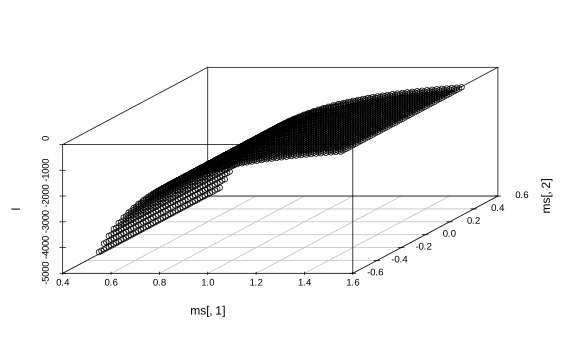
\includegraphics[width=1\linewidth]{Notas-Curso-Estadistica_files/figure-latex/unnamed-chunk-28-1} \end{center}

\textbf{Ejemplo}. \(X_1,\dots, X_n \stackrel{i.i.d}{\sim} \text{Unif}(0, \theta)\). Estime \(\theta\) \((\theta > 0)\). Suponga que \(x_i>0 \forall i\).

\[f(X|\theta) = \dfrac 1\theta \cdot 1_{[0,\theta]}(x)\]

La verosimilitud es
\[f_n(x|\theta) = \prod_{i=1}^{n} f(x_i|\theta) = \dfrac 1{\theta^n} \prod_{i=1}^n 1_{\{0\leq X_i\leq \theta\}} \quad 0\leq X_i \leq \theta \;\forall i\]

Vea que \(f_n(x|\theta)\) es válido si y solo si \(0\leq X_{(n)}\leq \theta\).

El valor de la muestra \(\{X_1,\dots, X_n\}\) en la \(i\)-ésima posición cuando los
datos se ordenan de menor a mayor se denota \(X_{(i)}\) (estadístico de orden). En
este caso, \(X_{(n)} = \max\{X_1,\dots, X_n\}\). Entonces \(\hat\theta_{MLE} = x_{(n)}\).

\textbf{Laboratorio:}

\begin{Shaded}
\begin{Highlighting}[]
\NormalTok{x \textless{}{-}}\StringTok{ }\KeywordTok{runif}\NormalTok{(}\DecValTok{100}\NormalTok{, }\DecValTok{0}\NormalTok{, }\DecValTok{2}\NormalTok{)}
\NormalTok{n \textless{}{-}}\StringTok{ }\KeywordTok{length}\NormalTok{(x)}

\NormalTok{theta \textless{}{-}}\StringTok{ }\KeywordTok{seq}\NormalTok{(}\FloatTok{1.5}\NormalTok{, }\FloatTok{2.5}\NormalTok{, }\DataTypeTok{length.out =} \DecValTok{1000}\NormalTok{)}

\NormalTok{L \textless{}{-}}\StringTok{ }\KeywordTok{numeric}\NormalTok{(}\DecValTok{1000}\NormalTok{)}
\ControlFlowTok{for}\NormalTok{ (k }\ControlFlowTok{in} \DecValTok{1}\OperatorTok{:}\DecValTok{1000}\NormalTok{) \{}
\NormalTok{    L[k] \textless{}{-}}\StringTok{ }\DecValTok{1}\OperatorTok{/}\NormalTok{theta[k]}\OperatorTok{\^{}}\NormalTok{n }\OperatorTok{*}\StringTok{ }\KeywordTok{prod}\NormalTok{(x }\OperatorTok{\textless{}}\StringTok{ }\NormalTok{theta[k])}
\NormalTok{\}}

\KeywordTok{plot}\NormalTok{(theta, L)}
\end{Highlighting}
\end{Shaded}

\begin{center}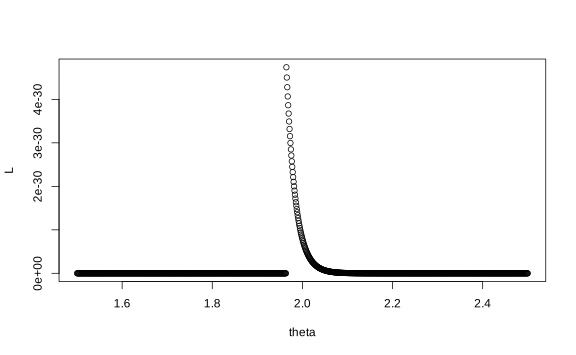
\includegraphics[width=1\linewidth]{Notas-Curso-Estadistica_files/figure-latex/unnamed-chunk-29-1} \end{center}

\hypertarget{propiedades-del-mle}{%
\section{Propiedades del MLE}\label{propiedades-del-mle}}

\hypertarget{propiedad-de-invarianza}{%
\subsection{Propiedad de invarianza}\label{propiedad-de-invarianza}}

\textbf{Teorema}. Si \(\hat\theta\) es el MLE de \(\hat\theta\) y si \(g\) es biyectiva,
entonces \(g(\theta)\) es el MLE de \(g(\theta)\).

\emph{Prueba}:

Sea \(\Gamma\) el espacio paramétrico \(g(\Omega)\). Como \(g\) es biyectiva entonces
defina \(h\) la inversa de \(g\colon \theta = h(\psi), \psi \in \Gamma\).

Reparametrizando la verosimilitud,
\[f_n(x|\theta) = f_n(x|h(\psi)). \]

El MLE de \(\psi:\hat\psi\) satisface que \(f_n(x|h(\hat\psi))\) es máximo.

Como \(f_n(x|\theta)\) se maximiza cuando \(\theta = \hat \theta\), entonces \(f_n(x|h(\psi))\) se
maximiza cuando \(\hat \theta = h(\psi)\) para algún \(\psi\).

Se concluye que \(\hat\theta = h(\hat\psi) \implies \hat\psi = g(\hat \theta)\).

\textbf{Ejemplo}: \(g(\theta) = \dfrac 1\theta\) es biyectiva si \(\theta > 0\). Así,

\begin{equation*} 
\frac{1}{\hat{\theta}} = \frac{1}{\frac{1}{\bar{X}_n}} =
\bar{X}_n \text{ es parámetro de la tasa.} 
\end{equation*}

¿Qué pasa si \(h\) no es biyectiva?

\textbf{Definicion (Generalización del MLE)}. Si \(g\) es una función de \(\theta\) y \(G\)
la imagen de \(\Omega\) bajo \(g\). Para cada \(t\in G\)
defina \[ G_t = \{\theta: g(\theta) = t\}\] Defina
\(L^*(t) = \displaystyle\max_{\theta\in G_t} \ln f_n(x|\theta)\). El MLE de \(g(\theta) (=\hat t)\)
satisface \(L^*(\hat t) = \displaystyle\max_{t \in G} L^*(t)\).

\textbf{Teorema}. Si \(\hat \theta\) es el MLE de \(\theta\) entonces \(g(\hat\theta)\) es el
MLE de \(g(\theta)\) (\(g\) es arbitraria).

\emph{Prueba}. Basta probar \(L^*(\hat t) = \ln f_n(x|\hat \theta)\). Se cumple que
\(\hat\theta\in G_{\hat t}\). Como \(\hat \theta\) maximiza \(f_n(x|\theta)\) \(\forall \theta\), también
lo hace si \(\theta \in G_{\hat t}\). Entonces \(\hat t = g(\hat \theta)\) (no pueden existir 2
máximos en un conjunto con la misma imagen).

\textbf{Ejemplos}.\(X_1,\dots, X_n \sim N(\mu, \sigma^2)\).

\begin{itemize}
\item
  Si \(h(\mu, \sigma^2) = \sigma\) (no es biyectiva) \(\implies h(\hat X_n,\hat\sigma^2) = \sqrt{\hat\sigma^2}\) es el MLE de \(\sigma\).
\item
  \(h(\mu,\sigma^2) = \dfrac{\sigma^*}{\mu}\) (coeficiente de variación). \(\dfrac{\hat{\sigma}}{\bar X_n}\) es el MLE de CV.
\item
  \(h(\mu, \sigma^2) = \mu^2 + \sigma^2\). \(\mathbb{E}[X^2] - \mu^2 = \sigma^2 \implies \mathbb{E}[X^2] = \mu^2 + \sigma^2\). El MLE de \(\mathbb{E}[X^2]\) es \(\bar X_n^2 + \hat \sigma ^2\).
\end{itemize}

\hypertarget{consistencia}{%
\subsection{Consistencia}\label{consistencia}}

Los estimadores bayesianos son de la forma
\[EB = W_1\mathbb{E}[\text{Previa}] + W_2\hat X_n.\]
El estimador bayesiano ``combina'' la esperanza de la previa y el \(\hat\theta_{MLE}\). El \(\hat\theta_{MLE}\) ``hereda la consistencia del estimador bayesiano''.

\[EB = W_1\mathbb{E}[\text{Previa}] + W_2 \hat\theta_{MLE}.\]
\textbf{Afirmación}. Bajo ``condiciones usuales'',
\[\hat\theta_{MLE} \xrightarrow[n\to \infty]{\mathbb P}\theta.\]

\hypertarget{cuxe1lculo-numuxe9rico}{%
\section{Cálculo numérico}\label{cuxe1lculo-numuxe9rico}}

\hypertarget{muxe9todo-de-los-momentos}{%
\subsection{Método de los momentos}\label{muxe9todo-de-los-momentos}}

\textbf{Ejemplo}. \(X_1,\dots, X_n \sim \Gamma(\alpha,1)\). Estime \(\alpha\).
\[f_n(x|\alpha) = \dfrac{1}{\Gamma(\alpha)}x^{\alpha-1}e^{-x}.\]

Verosimilitud: \(f_n(x|\alpha) = \dfrac 1 {\Gamma(\alpha)^n}(\prod x_i)e^{\sum x_i}\).

\begin{align*}
\dfrac{\partial}{\partial \alpha} L(\alpha|x) & = \dfrac{\partial}{\partial \alpha} \bigg[ -n\ln \Gamma(\alpha) + (\alpha-1)\ln(\pi x_i) - \sum x_i\bigg]\\
& = -n\dfrac{1}{\Gamma(\alpha)} \dfrac d{d\alpha}\Gamma(\alpha) + \ln (\prod x_i) = 0
\end{align*}

\textbf{Definición}. Asumimos que \(X_1,\dots, X_n \sim F\) indexada con un parámetro \(\theta \in \mathbb{R}^k\) y que al menos tiene \(k\) momentos finitos. Para \(j = 1,\dots, k\) sea \(\mu_j(\theta) = \mathbb{E}[X_1^j|\theta]\). Suponga que \(\mu(\theta) = (\mu_1(\theta),\dots,\mu_2(\theta))\) es biyectiva. Sea \(M\) la inversa de \(\mu\),
\[ M(\mu(\theta)) = \theta =M(\mu_1(\theta),\dots,\mu_2(\theta)) \]
y defina los momentos empíricos
\[ m_j = \dfrac 1n \sum_{i=1}^n X_i^j, \quad j=1,\dots, k.\]
El estimador según el método de los momentos es
\[\hat\theta = M(m_1,\dots,m_k).\]
Del ejemplo anterior, \(\mu_1(\alpha) = \mathbb{E}[x_1|\alpha] = \alpha\).Dado que \(m_1 = \hat x_n\), el sistema por resolver es
\[ \mu_1(\alpha) = m_1 \Longleftrightarrow \alpha = \bar x_n\]
El estimador por método de momentos es \(\hat \alpha = \bar X_n\).

\textbf{Ejemplo}. \(X_1,\dots, X_n \stackrel{i.i.d}{\sim} \Gamma(\alpha, \beta)\). La varianza de \(X\) es
\[ \dfrac{\alpha}{\beta^2} = \text{Var}X = \mathbb{E}[X^2]-\mathbb{E}[X]^2 = \mathbb{E}[X^2] - \dfrac{\alpha^2}{\beta^2}.\]
Se debe resolver el sistema
\[ \begin{cases}\mu_1(\theta) = \dfrac{\alpha}\beta = \bar X_n = m_1& (1)\\\mu_2(\theta) = \dfrac{\alpha(\alpha+1)}{\beta^2}=m_2 & (2)\end{cases}\]

De \((1)\), \(\alpha = m_1\beta\). Sustituyendo en \((2)\),

\[m_2 = \dfrac{m_1\beta(m_1\beta+1)}{\beta^2} = m_1^2+\dfrac{m_1}\beta = m_2\implies m_2-m_1^2 = \dfrac{m_1}{\beta}.\]
De esta manera,
\[ \hat\beta = \dfrac{m_1}{m_2-m_1^2},\quad  \hat\alpha = \dfrac{m_1^2}{m_2-m_1^2}\]
\textbf{Teorema}. Si \(X_1,X_2,\dots\) i.i.d con distribución indexada por \(\theta \in \mathbb{R}^k\). Suponga que los \(k\) momoentos teóricos son finitos \(\forall \theta\) y suponga que \(M\) es continua. Entonces el estimador por el método de momentos es consistente.

¿Cuál es el comportamiento en la distribución de \(\hat\theta\) cuando la muestra es grande?

Del teorema del límite central,
\[ \dfrac{\bar X_n-\theta}{\dfrac{\sigma}{\sqrt{n}}} = \dfrac{\sqrt{n}(\bar X_n-\theta)}{\sigma} \xrightarrow{d} N(0,1)\]
\[\text{Var}(\bar X_n) = \dfrac 1{n^2}\sum \text{Var}(X_1) = \dfrac{\sigma^2}n\]

Implica que se debe multiplicar la media muestral por una constante para hacer la desviación visibile y, con ello, hacer inferencia del parámetro.

\textbf{Caso general}. Si \(f(X|\theta)\) es ``suficientemente suave'' como función de \(\theta\), es puede comprobar que la verosimilitud tiende a una normal conforme \(n \to \infty\). Es decir,
\[ f(X|\theta)\propto \exp\Bigg[\dfrac{-1}{2\frac{V_n(\theta)}{n}}(\theta-\hat\theta)\Bigg], \quad n \to \infty\quad(*) \]
donde \(\hat\theta\) es el MLE de \(\theta\).

\[V_n(\theta)\xrightarrow[n\to \infty]{}V_{\infty}(\theta)<\infty\]

\textbf{Notas}:

\begin{enumerate}
\def\labelenumi{\arabic{enumi})}
\item
  Si \(n \to \infty\) la normal en \((*)\) tiene muchísima precisión y es concentrada alrededor de \(\hat\theta\).
\item
  En el caso bayesiano, ninguna previa en \(\theta\) puede anular el efecto en la verosimilitud cuando \(n\to \infty\).
\item
  Por \((*)\) el MLE se distribute asintóticamente como \[N\left(\theta, \dfrac{V_\infty(\theta)}{n}\right),\] \(Var(X_n)\xrightarrow[n\to \infty]{} 0\) y \(\mathbb{E}[X_n] = X \implies X_n \xrightarrow[n\to \infty]{\mathbb P} X\) (confirma que el MLE es consistente).
\end{enumerate}

\hypertarget{muxe9todo-delta}{%
\subsection{Método Delta}\label{muxe9todo-delta}}

Si \(Y_1,Y_2,\dots\) es una sucesión de variables aleatorias y sea \(F^*\) su c.d.f. continua. Sea \(\theta\in \mathbb R\) y \(\{a_n\}\) sucesión de números positivos tal que \(a_n \nearrow\infty\). Suponga que \(a_n(Y_n-\theta) \xrightarrow{d} F^*\). Si \(\alpha\) es una función tal que \(\alpha'(\theta)\ne 0\), entonces
\[\dfrac{a_n}{\alpha'(\theta)}[\alpha(Y_n)-\alpha(\theta)] \xrightarrow{d} F^*\]

\textbf{Ejemplo}. \(X_1,X_2,\dots\) i.i.d. de variables con media \(\mu\) y varianza \(\sigma^2\). Sea \(\alpha\) una función tal que \(\alpha'(\mu)\neq 0\). Por el T.L.C,
\[ \dfrac{\sqrt{n}}{\sigma}(X_n-\mu)\xrightarrow{d}N(0,1)\]

Entonces por el método Delta

\[ \dfrac{\sqrt{n}}{\sigma\alpha'(\mu)}[\alpha(\bar X_n)-\alpha(\mu)]\xrightarrow{d}N(0,1) \]

Si \(\alpha(\mu) = \dfrac 1\mu\) \((\mu\neq 0) \implies -\dfrac{1}{\mu^2} = \alpha'(\mu)\). Entonces por el método Delta

\[ \dfrac{\sqrt{n}}{\sigma}\mu^2\bigg[\dfrac 1{\bar X_n}-\dfrac 1\mu\bigg]\xrightarrow{d}N(0,1) \]

\textbf{Ejemplo}

Si \(X_1,X_2\dots \stackrel{i.i.d}{\sim} \text{Exp}(\theta)\). Sea \(T_n = \sum X_i \implies \hat\theta = \dfrac 1{\bar X_n} = \dfrac n{T_n}\).

Note que \(\dfrac{1}{\hat{\theta}} = \bar X_n\) y
\[ \dfrac{\sqrt{n}}{\sigma}\bigg[\bar X_n-\dfrac 1\theta\bigg]\xrightarrow[n\to\infty]{d}N(0,1) .\]

La varianza de una exponencial es \(\sigma^2 = \text{Var}(X_1) = \dfrac1{\theta^2}\), entonces
\[ \theta\sqrt{n}\bigg[\bar X_n-\dfrac 1\theta\bigg]\xrightarrow[n\to\infty]{d}N(0,1) .\]
El método Delta nos dice, con \(\alpha(\mu) = \dfrac 1\mu\), \(\alpha'(\mu) = -\dfrac 1{\mu^2}\), el comportamiento asintótico de MLE:

\begin{align*}
\dfrac{\theta\sqrt{n}}{\alpha'(1/\theta)}\bigg[\bar \alpha(X_n)-\alpha\left(\dfrac 1\theta\right)\bigg] 
& = \dfrac{\theta\sqrt{n}}{\dfrac{1}{1/\theta}}\bigg[ \dfrac 1{\bar X_n} -\theta\bigg]\xrightarrow[n\to\infty]{d}N(0,1) \\
& = \dfrac{\sqrt{n}}{\theta}\bigg[\dfrac 1{\bar X_n} -\theta\bigg]\xrightarrow[n\to\infty]{d}N(0,1) 
\end{align*}

El MLE \(\hat\theta = \dfrac 1{\bar X_n}\) es asintóticamente normal con media \(\theta\) y varianza \(\dfrac{V_n(\theta)}{n} = \dfrac{\theta^2}n\).

\textbf{Caso bayesiano}. Tome una previa conjugada \(\theta \sim \Gamma(\alpha,\beta)\), posterior \(\theta \sim \Gamma(\alpha+n,\beta+y)\), \(y = \sum X_i\). Supongamos que es entero positivo.
\[\Gamma(\alpha+n,\beta+y) \sim \sum_{i=1}^{\alpha+n}e^{\beta+y}\]
Por el T.L.C., la distribución posterior \(\theta|X\) se distribuye como una normal con media \(\dfrac{\alpha+n}{\beta+y}\) y varianza \(\dfrac{\alpha+n}{(\beta+y)^2}\). Tomando una previa poco informativa, (\(\alpha, \beta\) son pequeños), la media es
\[\dfrac ny = \dfrac 1{\bar X_1} = \hat\theta_{MLE}\] y la varianza
\[\dfrac 1{y^2/n} = \dfrac{\theta^2}n = \dfrac{V_n(\hat\theta)}{n}.\]

\hypertarget{laboratorio}{%
\section{Laboratorio}\label{laboratorio}}

Suponga que tenemos una tabla con los siguientes datos, los cuales representan la cantidad de giros hacia la derecha en cierta intersección.

\begin{Shaded}
\begin{Highlighting}[]
\NormalTok{(X \textless{}{-}}\StringTok{ }\KeywordTok{c}\NormalTok{(}\KeywordTok{rep}\NormalTok{(}\DecValTok{0}\NormalTok{, }\DecValTok{14}\NormalTok{), }\KeywordTok{rep}\NormalTok{(}\DecValTok{1}\NormalTok{, }\DecValTok{30}\NormalTok{), }\KeywordTok{rep}\NormalTok{(}\DecValTok{2}\NormalTok{, }\DecValTok{36}\NormalTok{), }\KeywordTok{rep}\NormalTok{(}\DecValTok{3}\NormalTok{, }
    \DecValTok{68}\NormalTok{), }\KeywordTok{rep}\NormalTok{(}\DecValTok{4}\NormalTok{, }\DecValTok{43}\NormalTok{), }\KeywordTok{rep}\NormalTok{(}\DecValTok{5}\NormalTok{, }\DecValTok{43}\NormalTok{), }\KeywordTok{rep}\NormalTok{(}\DecValTok{6}\NormalTok{, }\DecValTok{30}\NormalTok{), }\KeywordTok{rep}\NormalTok{(}\DecValTok{7}\NormalTok{, }
    \DecValTok{14}\NormalTok{), }\KeywordTok{rep}\NormalTok{(}\DecValTok{8}\NormalTok{, }\DecValTok{10}\NormalTok{), }\KeywordTok{rep}\NormalTok{(}\DecValTok{9}\NormalTok{, }\DecValTok{6}\NormalTok{), }\KeywordTok{rep}\NormalTok{(}\DecValTok{10}\NormalTok{, }\DecValTok{4}\NormalTok{), }\KeywordTok{rep}\NormalTok{(}\DecValTok{11}\NormalTok{, }
    \DecValTok{1}\NormalTok{), }\KeywordTok{rep}\NormalTok{(}\DecValTok{12}\NormalTok{, }\DecValTok{1}\NormalTok{)))}
\end{Highlighting}
\end{Shaded}

\begin{verbatim}
##   [1]  0  0  0  0  0  0  0  0  0  0  0  0  0  0  1  1  1  1  1  1  1  1  1  1  1
##  [26]  1  1  1  1  1  1  1  1  1  1  1  1  1  1  1  1  1  1  1  2  2  2  2  2  2
##  [51]  2  2  2  2  2  2  2  2  2  2  2  2  2  2  2  2  2  2  2  2  2  2  2  2  2
##  [76]  2  2  2  2  2  3  3  3  3  3  3  3  3  3  3  3  3  3  3  3  3  3  3  3  3
## [101]  3  3  3  3  3  3  3  3  3  3  3  3  3  3  3  3  3  3  3  3  3  3  3  3  3
## [126]  3  3  3  3  3  3  3  3  3  3  3  3  3  3  3  3  3  3  3  3  3  3  3  4  4
## [151]  4  4  4  4  4  4  4  4  4  4  4  4  4  4  4  4  4  4  4  4  4  4  4  4  4
## [176]  4  4  4  4  4  4  4  4  4  4  4  4  4  4  4  4  5  5  5  5  5  5  5  5  5
## [201]  5  5  5  5  5  5  5  5  5  5  5  5  5  5  5  5  5  5  5  5  5  5  5  5  5
## [226]  5  5  5  5  5  5  5  5  5  6  6  6  6  6  6  6  6  6  6  6  6  6  6  6  6
## [251]  6  6  6  6  6  6  6  6  6  6  6  6  6  6  7  7  7  7  7  7  7  7  7  7  7
## [276]  7  7  7  8  8  8  8  8  8  8  8  8  8  9  9  9  9  9  9 10 10 10 10 11 12
\end{verbatim}

Queremos ajustar esta tabla a una distribución Poisson con función de densidad

\[
\mathbb{P}(X=x) = \frac{\lambda^x e^{-\lambda}}{x!} 
\]

Se puede probar que teórico de máxima verosimilitud para \(\lambda\) es \(\overline{X}\) (Tarea). Queremos estimar este parámetro alternativamente maximizando la función de verosimilitud.

Primero veamos la forma de los datos,

\begin{Shaded}
\begin{Highlighting}[]
\KeywordTok{hist}\NormalTok{(X, }\DataTypeTok{main =} \StringTok{"histograma del número de giros a la derecha"}\NormalTok{, }
    \DataTypeTok{right =} \OtherTok{FALSE}\NormalTok{, }\DataTypeTok{prob =} \OtherTok{TRUE}\NormalTok{)}
\end{Highlighting}
\end{Shaded}

\begin{center}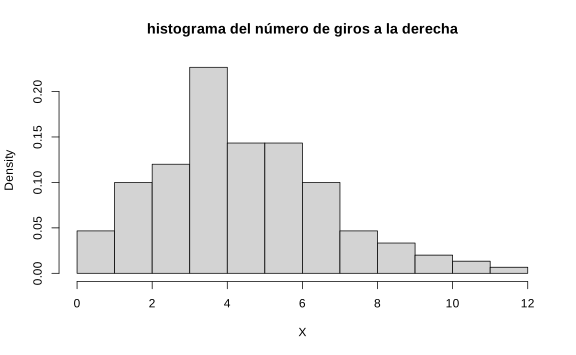
\includegraphics[width=1\linewidth]{Notas-Curso-Estadistica_files/figure-latex/unnamed-chunk-31-1} \end{center}

Definamos la función correspondiente a \(-\log(\mathbb{P}(X=x))\)

\begin{Shaded}
\begin{Highlighting}[]
\NormalTok{n \textless{}{-}}\StringTok{ }\KeywordTok{length}\NormalTok{(X)}
\NormalTok{negloglike \textless{}{-}}\StringTok{ }\ControlFlowTok{function}\NormalTok{(lambda) \{}
\NormalTok{    n }\OperatorTok{*}\StringTok{ }\NormalTok{lambda }\OperatorTok{{-}}\StringTok{ }\KeywordTok{sum}\NormalTok{(X) }\OperatorTok{*}\StringTok{ }\KeywordTok{log}\NormalTok{(lambda) }\OperatorTok{+}\StringTok{ }\KeywordTok{sum}\NormalTok{(}\KeywordTok{log}\NormalTok{(}\KeywordTok{factorial}\NormalTok{(X)))}
\NormalTok{\}}
\end{Highlighting}
\end{Shaded}

Para encontrar el parámetro deseado, basta minimizar la función \texttt{negloglike} usando el la instrucción de optimización no lineal \texttt{nlm}.

\begin{Shaded}
\begin{Highlighting}[]
\NormalTok{lambda.hat \textless{}{-}}\StringTok{ }\KeywordTok{nlm}\NormalTok{(negloglike, }\DataTypeTok{p =} \KeywordTok{c}\NormalTok{(}\FloatTok{0.5}\NormalTok{), }\DataTypeTok{hessian =} \OtherTok{TRUE}\NormalTok{)}
\end{Highlighting}
\end{Shaded}

Aquí el valor \texttt{p\ =\ c(0.5)} representa un valor inicial de búsqueda y \texttt{hessian\ =\ TRUE} determina el cálculo explícito de la segunda derivada.

Compare el resultado de \texttt{lambda.hat\$estimate} con \texttt{mean(X)}.

\begin{Shaded}
\begin{Highlighting}[]
\NormalTok{lambda.hat}\OperatorTok{$}\NormalTok{estimate}
\end{Highlighting}
\end{Shaded}

\begin{verbatim}
## [1] 3.893331
\end{verbatim}

\begin{Shaded}
\begin{Highlighting}[]
\KeywordTok{mean}\NormalTok{(X)}
\end{Highlighting}
\end{Shaded}

\begin{verbatim}
## [1] 3.893333
\end{verbatim}

\hypertarget{estaduxedsticos-suficientes-y-criterio-de-factorizaciuxf3n}{%
\chapter{Estadísticos Suficientes y Criterio de Factorización}\label{estaduxedsticos-suficientes-y-criterio-de-factorizaciuxf3n}}

\hypertarget{estaduxedsticos-suficientes}{%
\section{Estadísticos suficientes}\label{estaduxedsticos-suficientes}}

Una función de verosimilitud se va a describir a través de un número. El
objetivo es buscar un estadístico \(T=r(X_1,\dots,X_n)\) que resuma de manera
óptima la información de \(X_1,\dots,X_n\)

\textbf{Definición}. Sea \(X_1,\dots,X_n\) una muestra indexada por \(\theta\). Sea \(T\)
un estadístico, suponga que para cada \(\theta \in \Omega\) y para cada \(t\) en la imagen
de \(T\), \(X_1\cdots X_n|T=t\) depende solamente de \(t\) y no de \(\theta\). Entonces \(T\)
es suficiente.

\hypertarget{teorema-de-factorizaciuxf3n-de-fisher}{%
\section{Teorema de Factorización de Fisher}\label{teorema-de-factorizaciuxf3n-de-fisher}}

\textbf{Teorema}. Si \(X_1,\dots,X_n\) es una muestra aleatoria de \(f(X|\theta)\), el
parámetro \(\theta\) es desconocido. Un estadístico \(T=r(X_1,\dots,X_n)\) es
suficiente si y solo si \[f_n(x|\theta) = u(x)v(r(x),\theta)\;\forall x\in
\mathbb R, \; \forall \theta \in \mathbb R.\]

\emph{Prueba} (Discreta). \(f_n(x|\theta) = \mathbb P(X=x|\theta)\)

``\(\Leftarrow\)'' Sea \(A(t) = \{x\in \mathbb R| r(x) =t\}\). Para \(\theta \in \mathbb R\), \(x\in A(t)\),

\begin{align*}
\mathbb P(X=x|T=t) 
& = \dfrac{\mathbb P(X=x \cap T=t)}{\mathbb P (T=t)} \\ 
&= \dfrac{f_n(x|\theta, T=t)}{\displaystyle\sum_{y \in A(t)}f_n(y|\theta)} \\
& = \dfrac{u(x)v(r(x),\theta)}{\displaystyle\sum_{y \in A(t)} u(y)v(r(y),\theta)} \\ 
& = \dfrac{u(x)v(t,\theta)}{\displaystyle v(t,\theta)\sum_{y \in A(t)} u(y)} \text{(Como \(y\in A(t)\) entonces \(r(y) = t\) que es constante.)}\\ 
&= \dfrac{u(x)}{\displaystyle\sum_{y \in A(t)}u(y)}
\end{align*}

no depende de \(\theta\).

Si \(x\notin A(t) \implies \mathbb P(X=x|T=t) = 0\) no depende de \(\theta\).

``\(\Rightarrow\)'' Si \(T\) es un estadístico suficiente, \(u(x) = \mathbb P(X=x|T=t)\) no depende de \(\theta\). Sea \(v(t,\theta) = \mathbb P_{\theta}(T=t)\). Entonces

\[ f_n(x|\theta) = \mathbb P (X=x|\theta) = \dfrac{\mathbb P(X=x|\theta)}{\mathbb P(T=t)}\mathbb P(T=t) = u(x)v(t,\theta).\]

\textbf{Consecuencia}: \(f_n(x|\theta) \propto v(r(x),\theta)\) (\(u(x)\) es una constante con respecto a \(\theta\)). Aplicando el teorema de Bayes,
\[ \pi(\theta|x) \propto \pi(\theta)v(r(x),\theta).\]

\textbf{Corolario}. Un estadístico \(r(x)\) es suficiente si y solo si no importa cuál previa de \(\theta\) se use, la posterior depende solamente de \(r(x)\) a través de los datos.

\textbf{Ejemplo}. \(X_1,\dots, X_n \sim \text{Poi}(\lambda)\),

\[f_n(x|\theta) = \prod_{i=1}^n \dfrac{e^{-\lambda}}{x_i!} = \dfrac{e^{-\lambda n} \lambda ^{\sum x_i (\;= r(x))}}{\prod x_i!} = \underbrace{\dfrac{1}{\prod_{i=1}^n x_i!}}_{u(x)} \underbrace{e^{-\lambda n}\lambda^{r(x)}}_{v(r(x),\lambda)}\]

Si \(x_i < 0\) para al menos un \(i\), entonces \(f_n(x|\theta) = 0\). Tome \(u(x) = 0\). Por el teorema de factorización, \(r(x) = \sum x_i\) es un estadístico suficiente para \(\lambda\).

\textbf{Ejemplo}. \(X_1,\dots, X_n \sim f(x|\theta)\)
\[ f(x|\theta) = \begin{cases}\theta x^{\theta-1} & 0<x< 1\\ 0 & \text{otro caso}\end{cases}\]

Verosimilitud: (\(0<x_i<1\) \(\forall i\))

\[ f_n(x|\theta) = \theta^n\bigg[\underbrace{\prod(x_i)}_{r(x)}\bigg]^{\theta-1}  = \underbrace{\theta^n(r(x))^{\theta-1}}_{v(r(x),\theta)}\cdot \underbrace{1}_{u(x)}\]

Por el teorema de factorización \(r(x) = \prod x_i\) es un estadístico suficiente.,

\textbf{Ejemplo}. \(X_1,\dots, X_n \sim N(\mu, \sigma^2)\) (\(\sigma^2\) conocido).

\begin{align*} 
f_n(x|\theta) & = (2\pi\sigma^2)^{-n/2} \exp\bigg[-\dfrac{1}{2\sigma^2}\sum_{i=1}^n(X_i-\mu)^2\bigg] \\
& = (2\pi\sigma^2)^{-n/2} \exp\bigg[-\dfrac{1}{2\sigma^2}\underbrace{\sum_{i=1}^n X_i^2}_{r_2(x)}+ \dfrac{\mu}{\sigma^2}\underbrace{\sum_{i=1}^n X_i}_{r_1(x)} - \dfrac{\mu^2 n}{2\sigma^2} \bigg]
\end{align*}

Tome \[u(x) = (2\pi\sigma^2)^{-n/2}\exp\bigg[-\dfrac{1}{2\sigma^2} \displaystyle\sum_{i=1}^n X_i^2\bigg],\]
\[ v(r_{1}(x),\mu) = \exp\bigg[\dfrac{\mu}{\sigma^2}r_{1}(x) - \dfrac{n\mu^2}{2\sigma^2}\bigg]. \]

Por teorema de factorización, \(r_{1}(x)=\sum X_i\) es un estadístico suficiente para \(\mu\).

Con \(\sigma^2\) desconocido, \(\theta = (\mu,\sigma^2)\), tome \(u(x) = 1\),
\[ v(r_1(x),r_2(x),\theta) = (2\pi\sigma^2)^{-n/2}\exp\bigg[\dfrac{-r_2(x)}{2\sigma^2} + \dfrac{\mu r_1(x)}{\sigma^2}- \dfrac{n\mu^2}{2\sigma^2}\bigg] \]
Entonces
\[ (r_1(x),r_2(x)) = \left(\sum{x_i},\sum x_i ^2\right) \]
es un estadístico suficiente para \((\mu, \sigma^2)\).

\textbf{Ejemplo}. \(X_1,\dots, X_n \stackrel{i.i.d}{\sim}\text{Unif}(0,\theta)\), \(\theta>0\), \(f(x|\theta) = 1_{[0,\theta]}(x)\dfrac 1\theta\).
\[f_n(x|\theta) = \prod_{i=1}^n 1_{[0,\theta]}(x_i)\left(\dfrac 1\theta \right) \]

\emph{Nota:} si al menos uno de los \(x_i<0\) o \(x_i>\theta\), \(u(x) = 0\) \((f(x|\theta) = 0)\) (Trivial).

Si \(0<x_i<\theta\) \(\forall i \implies f_n(x|\theta) = 1_{[0,\theta]}(\max\{x_i\})\left(\dfrac 1\theta \right)^n.\)

Si \(T = r(x) = X_{(n)} \implies f_n(x|\theta) = u(x)v(r(x),\theta)\), \(u(x) = 1\). Por teorema de factorización, \(r(x) = x_{(n)}\) es un estadístico suficiente para \(\theta\).

\hypertarget{estaduxedstico-suficiente-multivariado.}{%
\section{Estadístico suficiente multivariado.}\label{estaduxedstico-suficiente-multivariado.}}

Si \(\theta \in \mathbb R^k\), \(k\geq 1\) se necesita al menos \(k\) estadísticos
\((T_1,\dots,T_k)\) para cada \(i=1,\dots,k\), \(T_i = r_i(X_1,\dots, X_n)\).

\textbf{Definición}. Suponga que para cada \(\theta\in \Omega\) y \((t_1,\dots, t_k) \in \mathbb R^k\) valor del estadístico \((T_1,\dots,T_k)\), la distribución condicional de
\(X_1,\dots, X_n\) dado \((T_1,\dots,T_k) = (t_1,\dots, t_k)\) no depende de
\(\theta\), entonces \((T_1,\dots,T_k)\) es un \textbf{estadístico suficiente} para
\(\theta\).

\textbf{Criterio de factorización}:

\[ f_n(x|\theta) = u(x)v(r_1(x),\dots,r_k(x),\theta) \Leftrightarrow T = (r_1(x),\dots,r_k(x)) \text{ es
suficiente}\]

Si \((T_1,\dots,T_k)\) es suficiente para \(\theta\) y si \((T_1',\dots,T_k') = g(T_1,\dots,T_k)\) donde \(g\) es biyectiva, entonces \((T_1',\dots,T_k')\) es
suficiente para \(\theta\). \[ u(x)v(r(x)|\theta) = u(x)v(g^{-1}(g(r(x))),\theta).\]

\textbf{Ejemplo}. Considere los siguiente

\begin{align*}
T_1 &= \sum_{i=1}^{n} X_i \\
T_2 &= \sum_{i=1}^{n} X_i^2 \\
T_1' & = \frac{1}{n} \sum_{i=1}^{n} X_i \\
T_2' &= \frac{1}{n} \sum_{i=1}^{n} (X_i - \overline{X}_n) ^{2}
\end{align*}

Entonces defina la siguiente función
\[
(T_1',T_2') = g(T_1,T_2) =
\left(\dfrac{1}{n}T_1,\dfrac{1}{n}T_2 - \dfrac{1}{n^2}T_1^2\right).
\]

De la primera entrada,
\[ T_1' = \dfrac 1n T_1 \implies T_1 = nT_1'.\]
De la segunda,
\begin{align*}
T_2' = \dfrac 1n T_2 - \dfrac 1{n^2} & = \dfrac 1n \sum X_i^2 - \left(\dfrac 1n \sum X_i\right)^2\\
& = \dfrac 1n \sum X_i^2 - 2X_i\bar X_n^2 + \bar X_n \\
& = \dfrac 1n \sum(X_i-\bar X_n)^2 = \hat\sigma_n^2
\end{align*}
Como \(g\) es biyectiva entonces \((\bar X_n, \sigma_n^2)\) es un estadístico suficiente para \((\mu,\sigma^2)\).

\textbf{Ejemplo}. \(X_1,\dots, X_n \sim \text{Unif}(a,b)\), \(a<b\). Encuentre un estadístico suficiente.

\begin{enumerate}
\def\labelenumi{\arabic{enumi}.}
\item
  Si \(x_i \leq a\) o \(x_i>b\), tome \(u(x) = 0\).
\item
  Si \(a< x_i <b\) \(\forall i\),

  \begin{enumerate}
  \def\labelenumii{\alph{enumii}.}
  \item
    \(x_i > a\) \(\forall i \Leftrightarrow x_{(1)}>a\).
  \item
    \(x_i < b\) \(\forall i \Leftrightarrow x_{(n)}<b\).
  \end{enumerate}
\end{enumerate}

La verosimilitud es de la forma

\[f_n(x|(a,b)) = \prod_{i=1}^n1_{[a,b]}(x_i) = \underbrace{\dfrac 1{(b-a)^n} 1_{\{(z,w): z>a, w<b\}}(X_{(1)},X_{(n)})}_{v(r_1(x),r_2(x),(a,b))}\cdot \underbrace{1}_{u(x)}\]

Por teorema de factorización \((r_{1}(x), r_{2}(x)) = (X_{(1)},X_{(n)})\) es un
estadístico suficiente para \((a,b)\).

\hypertarget{estaduxedsticos-minimales}{%
\section{Estadísticos minimales}\label{estaduxedsticos-minimales}}

\textbf{Idea:} un estadístico suficiente que garantice una partición de \(\mathcal X\)
(espacio muestral) de la manera más simple posible.

\textbf{Definición (Estadístico de orden)}. Sean \(X_1,\dots, X_n \stackrel{i.i.d}{\sim} f\). Al ordenar los datos

\[(Y_1,\dots,Y_n) = (X_{(1)},\dots,X_{(n)}) \text { tal
que } Y_1<\dots<Y_n\]

\textbf{Nota}: \((X_{(1)},\dots,X_{(n)})\) es un estadístico suficiente de \(\theta\).

\textbf{Ejemplo}. \(X_1,\dots, X_n \sim \text{Cauchy}(\alpha)\).
\[ f(x) = \dfrac1\pi[1+(x-\alpha)^2]^{-1}, x\in\mathbb R\]

Busque un estimador suficiente para \(\alpha \in \mathbb R\).

\[ f_n(x|\alpha) = \prod(x|\alpha) = \dfrac 1\pi [1+(x_i-\alpha)^2]^{-1} = \underbrace{\dfrac 1{\pi^n}}_{u(x)}\underbrace{\prod_{i=1}^n[1+(x_i-\alpha)^2]^{-1} }_{v(y,\alpha)} \]
donde \(y = (X_{(1)},\dots,X_{(n)})\) es suficiente para \(\alpha\).

\textbf{Ejercicio}: estime \(\alpha\) usando R o usando método de momentos.

\textbf{Definición}. Un estadístico \(T\) es \textbf{suficiente minimal} si \(T\) es
suficiente y es función de cualquier otro estadístico suficiente.

\textbf{Teorema}. Si \(T = r(X_1,\dots, X_n)\) es un estadístico suficiente para
\(\theta\), entonces el MLE \(\hat\theta\) de \(\theta\) depende de \(X_1,\dots, X_n\)
solamente a través de \(T\). Además, si \(\hat \theta\) es suficiente entonces \(\hat \theta\) es minimal.

\emph{Prueba}. Por teorema de factorización, \(f_n(x|\theta) = u(x)v(r(x),\theta)\) de \(T =r(x)\)
es suficiente y
\[\hat\theta = \operatorname*{argmax}_\theta f_n(x|\theta) = \operatorname*{argmax}_\theta v(r(x),\theta), \quad (\Delta)\]

Como \(\hat\theta = g(T)\) para cualquier \(T\) estadístico suficiente, entonces \(\hat\theta\) es minimal.

\textbf{Teorema}. Si \(T = r(X_1,\dots, X_n)\) es un estadístico suficiente para
\(\theta\) entonces el estimador bayesiano (bajo una escogencia de \(L\)) depende de
\(X_1,\dots, X_n\) solamente a través de \(T\) (el estimador bayesiano es minimal).

\emph{Prueba}. Sustituya \((\Delta)\) por \(\pi(\theta|x) \propto v(r(x),\theta)\cdot\pi(\theta)\). Como cualquier
estimador bayesiano depende de \(\pi(\theta|x)\), cualquier estimador bayesiano depende
e los datos a través de \(r(x)\).

\hypertarget{mejorando-estimadores}{%
\section{Mejorando estimadores}\label{mejorando-estimadores}}

\textbf{Idea:} ¿Será posible mejorar un estimar que no es suficiente?

¿Existirá otra medida de comparación entre estimadores?

Considere una \textbf{función de riesgo o pérdida}
\[ R(\theta,\delta) = \mathbb E[(\delta(x)-\theta) ^2]\]
Si \(\delta(x)\) estima una característica de \(F\):
\[ R(\theta,\delta) = \mathbb E[(\delta(x)-h(\theta))^2]\quad (\Delta\Delta)\]
donde \(h\) es la característica.

\textbf{Nota:} la función de riesgo puede ser calculada con una posterior \(\pi(\theta|X)\).

\textbf{Definición}.

\begin{itemize}
\item
  Decimos que \(\delta\) es \textbf{inadmisible} si \(\exists \delta_0\) (otro estimador) tal que
  \(R(\theta, \delta_{0}) \leq R(\theta,\delta)\) \(\forall \theta \in \Omega\).
  deltadelta
\item
  Decimos que \(\delta_0\) \textbf{``domina''} a \(\delta\) en el caso anterior.
\item
  Decimos que \(\delta_0\) es admisible si no existe otro estimador que domine a
  \(\delta_0\).
\item
  A \((\Delta \Delta)\) se le llama \textbf{MSE} o \textbf{error cuadrático medio}.
\end{itemize}

\textbf{Teorema (Rao-Blackwell)}. Sea \(\delta(X)\) un estimador y \(T\) un estadístico
suficiente para \(\theta\) y sea \(\delta_0 = \mathbb E[\delta(X)|T]\). Entonces \[ R(\theta,\delta_0) \leq
R(\theta,\delta) \; \forall \theta \in \Omega\]

\emph{Prueba}. Por la desigualdad de Jensen,
\[ \mathbb E_\theta[(\delta(x)-\theta)^2] \geq (E_\theta[(\delta(x)-\theta)])^2. \]
También,
\[\mathbb E[(\delta(x)-\theta)^2|T] \geq (E[(\delta(x)|T)]-\theta)^2 = (\delta_0(T)-\theta)^2.\]

Entonces,
\[ \mathbb E[(\delta(x)-\theta)^2] \leq \mathbb E[\mathbb E[(\delta(x)-\theta)^2|T]] = \mathbb E[(\delta(x)-\theta)^2] = R(\theta,\delta).\]

\textbf{Nota}. Si cambiamos a \(R(\theta,\delta) = \mathbb E[|\delta(x)-\theta|]\) (error medio absoluto), el resultado anterior es cierto.

\textbf{Ejemplo}. Sean \(X_1,\dots, X_n \stackrel{i.i.d}{\sim} \text{Poisson}(\theta)\) donde \(\theta\) es la tasa de ``visitas'' de clientes por hora.

Numericamente podemos hacer el ejemplo con \(\theta = 2\) y una muestra de \(n = 10000\),

\begin{Shaded}
\begin{Highlighting}[]
\NormalTok{X \textless{}{-}}\StringTok{ }\KeywordTok{rpois}\NormalTok{(}\DataTypeTok{n =} \DecValTok{10000}\NormalTok{, }\DataTypeTok{lambda =} \DecValTok{2}\NormalTok{)}
\KeywordTok{head}\NormalTok{(X, }\DecValTok{20}\NormalTok{)}
\end{Highlighting}
\end{Shaded}

\begin{verbatim}
##  [1] 3 2 3 4 1 5 3 0 3 0 0 0 5 0 2 5 0 3 2 2
\end{verbatim}

\begin{Shaded}
\begin{Highlighting}[]
\KeywordTok{hist}\NormalTok{(X)}
\end{Highlighting}
\end{Shaded}

\begin{center}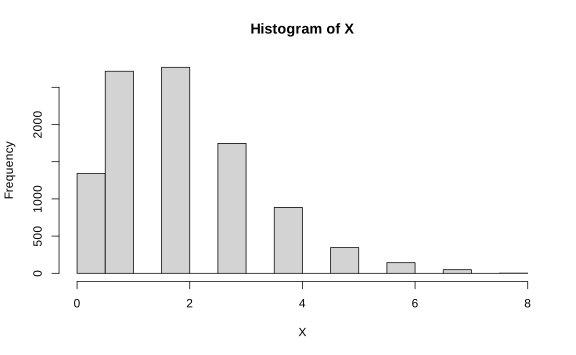
\includegraphics[width=1\linewidth]{Notas-Curso-Estadistica_files/figure-latex/unnamed-chunk-36-1} \end{center}

A partir de la verosimilitud,
\[f_n(X|\theta) = \dfrac{e^{-\theta n} \theta^{\sum X_i}}{\prod X_i!} \]
se tiene que \(T=\sum X_i\) es un estadístico suficiente para \(\theta\).

Sea \(Y_i = \begin{cases} 1 & \text{si } X_i = 1\\ 0 & \text{si } X_i \ne 1\end{cases}\).

Esta \(Y\) se calcula de la forma

\begin{Shaded}
\begin{Highlighting}[]
\NormalTok{Y \textless{}{-}}\StringTok{ }\NormalTok{X }\OperatorTok{==}\StringTok{ }\DecValTok{1}
\KeywordTok{head}\NormalTok{(Y, }\DecValTok{10}\NormalTok{)}
\end{Highlighting}
\end{Shaded}

\begin{verbatim}
##  [1] FALSE FALSE FALSE FALSE  TRUE FALSE FALSE FALSE FALSE FALSE
\end{verbatim}

El objetivo es estimar \(p\) donde \(p\) es la probabilidad de que \(X_i =1\) (solo llegue un cliente por hora). Un estimador de \(p\) (MLE) es
\[\delta(x) = \dfrac{\sum Y_i}{n}\]

\begin{Shaded}
\begin{Highlighting}[]
\NormalTok{(delta \textless{}{-}}\StringTok{ }\KeywordTok{mean}\NormalTok{(Y))}
\end{Highlighting}
\end{Shaded}

\begin{verbatim}
## [1] 0.264
\end{verbatim}

¿Es el óptimo?

Calculamos
\[\mathbb E[\delta(x)|T] = \dfrac 1n \sum_{i=1}^n \mathbb E (Y_i|T)\]
Vea que
\begin{align*}
\mathbb E[Y_i|T = t] = \mathbb P(X_i = 1 | T = t) & = \dfrac{\mathbb P(X_i = 1, T=t)}{\mathbb P(T=t)}\\
& = \dfrac{\mathbb P(X_i = 1, \sum_{j\ne i} X_j = t-1)}{\mathbb P(T=t)}\\
& = \dfrac{\mathbb P(X_i = 1) \mathbb P(\sum_{j\ne i} X_j = t-1)}{\mathbb P(T=t)} = \Delta
\end{align*}

\begin{itemize}
\item
  \(\mathbb P(X_i = 1) = \theta e^{-\theta}\)
\item
  \(\mathbb P(\sum_{j\ne i}X_j = t-1) = e^{-(n-1)\theta}\dfrac{((n-1)\theta)^{t-1}}{(t-1)!}\)
\item
  \(\mathbb P(T=t) = e^{-n\theta}\dfrac{(n\theta)^t}{t!}\)
\end{itemize}

Entonces,
\begin{align*}
\Delta = \dfrac{\theta e^{-n\theta}\dfrac{((n-1)\theta)^{t-1}}{(t-1)!}}{e^{-n\theta}\dfrac{(n\theta)^t}{t!}} = \dfrac tn \left(1-\dfrac 1n\right)^{t-1} = G\left(\dfrac tn\right)
\end{align*}

es el estadístico con MSE mínimo.

\begin{Shaded}
\begin{Highlighting}[]
\NormalTok{T \textless{}{-}}\StringTok{ }\KeywordTok{sum}\NormalTok{(X)}
\NormalTok{n \textless{}{-}}\StringTok{ }\KeywordTok{length}\NormalTok{(X)}
\NormalTok{(delta\_}\DecValTok{0}\NormalTok{ \textless{}{-}}\StringTok{ }\NormalTok{(T}\OperatorTok{/}\NormalTok{n) }\OperatorTok{*}\StringTok{ }\NormalTok{(}\DecValTok{1} \OperatorTok{{-}}\StringTok{ }\DecValTok{1}\OperatorTok{/}\NormalTok{n)}\OperatorTok{\^{}}\NormalTok{(T }\OperatorTok{{-}}\StringTok{ }\DecValTok{1}\NormalTok{))}
\end{Highlighting}
\end{Shaded}

\begin{verbatim}
## [1] 0.2707382
\end{verbatim}

En este caso \(\delta_0\) es mejor que \(\delta\) bajo una pérdida cuadrática.

\hypertarget{distribuciuxf3n-muestral-de-un-estaduxedstico}{%
\chapter{Distribución muestral de un estadístico}\label{distribuciuxf3n-muestral-de-un-estaduxedstico}}

\hypertarget{distribuciuxf3n-muestral}{%
\section{Distribución muestral}\label{distribuciuxf3n-muestral}}

\textbf{Definición}. Suponga que \(X_1,\dots,X_n\) es una muestra con parámetro
\(\theta\) con parámetro \(\theta\) (desconocido). Sea \(T=r(X_1,\dots,X_n,\theta)\). La
distribución de \(T\) dado \(\theta\) se llama \textbf{distribución muestral}.

\textbf{Ejemplo}. Si \(X_1,\dots,X_n \sim N(\mu,\sigma^2)\). El MLE de \(\mu\) es

\begin{equation*}
\bar X_n =\dfrac 1n \sum_{i=1}^n X_i.
\end{equation*}

La distribución muestral del estadístico \(\bar X_n\) es

\[
\bar X_n \sim N\left(\mu, \dfrac{\sigma^2}n \right)
\]

\begin{itemize}
\item
  \(\mathbb E[\bar X_n] = \dfrac 1n\displaystyle\sum_{i=1}^n\mathbb E[X_i] = \dfrac 1n\cdot n \mathbb E[X_1] = \mu\).
\item
  \(\text{Var}(\bar X_n) = \text{Var}\left(\dfrac 1n \displaystyle\sum_{i=1}^n X_i\right) = \dfrac{1}{n^2}\cdot n\cdot \text{Var}(X_1) = \dfrac{\sigma^2}n\).
\end{itemize}

\textbf{Ejemplo}. \(X_i:\) tiempo de vida de un aparato. \(X_1,\dots,X_n \stackrel{i.i.d}{\sim} \text{Exp}(\theta)\). La previa de \(\theta\) es \(\Gamma(1,2)\). Solamente
observamos \(n=3\). La posterior sería

\[
\theta|X \sim \Gamma(1+3,2+\sum_{i=1}^3 X_i). 
\]

El estimador bayesiano, bajo pérdida cuadrática, es
\[
\mathbb E[\theta|X] = \dfrac 4{2+\sum X_i} = \hat\theta
\]

\textbf{Problema:} estimar \(\mathbb P(|\hat\theta-\theta|<0.1)\).

Note que

\begin{align*}
\mathbb P(|\hat\theta-\theta|<0.1)
&= \mathbb E [1_{|\hat\theta-\theta|<0.1|\theta)}] \\
&= \mathbb E[\mathbb E [1_{|\hat\theta-\theta|<0.1|\theta)}\vert \theta]] \\
&= \mathbb E[\mathbb P(|\hat\theta-\theta|<0.1|\theta)]
\end{align*}

Debemos definir primero cuál es la función de distribución de \(\hat{\theta}\).

\begin{align*}
F_{\hat{\theta}}(t|\theta) = \mathbb P(\hat\theta\leq t|\theta)&= \mathbb
P\left( \dfrac 4{2+T}\leq t\bigg|\theta\right) \\ & = \mathbb P\left( 2+T \geq
\dfrac 4t\bigg|\theta\right)\\ & = \mathbb P\left( T \geq \dfrac
4t-2\bigg|\theta\right)
\end{align*}

\textbf{Nota: Recuerde que sumas de exponenciales es una gamma. (Ver teorema 5.7.7)}

Entonces \(T=\sum_{i=1}^{3}X_{i}\sim \Gamma(3,\theta)\), por lo que \(F(t|\theta) = 1-G_{\Gamma(3,0)}\left( \dfrac 4t-2\right)\). Aqui denotamos como \(G\) a la
distribución de \(T\).

De esta manera,

\begin{align*}
\mathbb P[|\hat\theta-\theta|<0.1|\theta]  
& = \mathbb P [-0.1+\theta < \hat\theta < 0.1 +\theta|\theta]\\
& = G_{\Gamma(3,\theta)}\left(\dfrac 4{-0.1+\theta} - 2\right)-G_{\Gamma(3,\theta)}\left(\dfrac 4{0.1+\theta} - 2\right)
\end{align*}

y se toma la esperanza para estimar la esperanza. Este valor no se puede estimar
de forma cerrada, sino que se podría aproximar mediante una simulación

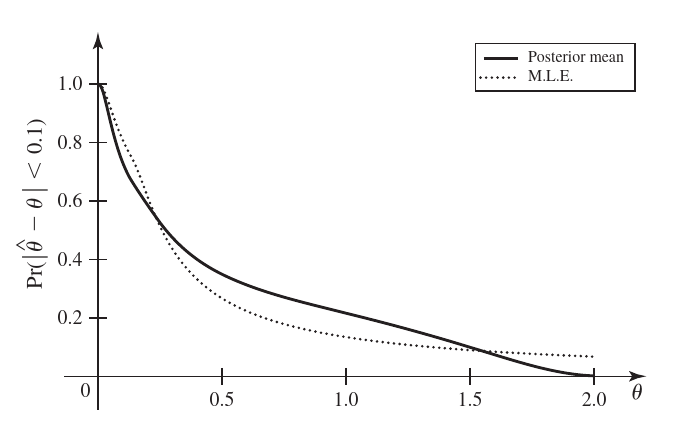
\includegraphics{./images/gamma_mle_vs_posterior.png}

Otra solución es estimar \(\theta\) usando el MLE \(\hat{\theta} = \frac{3}{T}\). Se
podría construir esa probabilidad de forma que no dependa de \(\theta\).

\[
\mathbb P \left(\bigg| \underbrace{\dfrac{\hat\theta_{MLE}}\theta-1}_{\text{Cambio
relativo}} \bigg| < 0.1\bigg|\theta \right) = \mathbb P \left( \bigg| \dfrac{3}{\theta
T}-1 \bigg| < 0.1 \bigg| \theta \right) = \Delta \]

Si \(T\sim\Gamma(3,\theta) \implies \theta T \sim \Gamma(3,1)\).

Por lo tanto,
\[
\Delta = \mathbb P \left(0.9<\dfrac 3{\theta T}<1.1\bigg|\theta\right) = \mathbb P \left(\dfrac 3{1.1}<\theta T<\dfrac 3{0.9}\right) = 13,4\%
\]

\hypertarget{distribuciuxf3n-chi2}{%
\section{\texorpdfstring{Distribución \(\chi^2\)}{Distribución \textbackslash chi\^{}2}}\label{distribuciuxf3n-chi2}}

\textbf{Definición}. Para \(m>0\) definimos
\[
\chi^2_m \sim \Gamma\left(\dfrac m2, \dfrac 12 \right)
\]

la distribución \textbf{chi-cuadrado} con \(m\) grados de libertad.

\textbf{Propiedades}:

\begin{itemize}
\item
  \(\mathbb E[X] = m\).
\item
  \(\text{Var} (X) = 2m\).
\item
  Para \(X_i \sim \chi^2_{m_i}\), \(i = 1,\dots, k\), independientes, entonces
\end{itemize}

\[\sum_{i=1}^k X_i \sim \chi^2_{\sum m_i}\]

\begin{itemize}
\item
  Si \(X\sim N(0,1) \implies Y = X^2\sim \chi^2_1\).
\item
  Si \(X_i \stackrel{i.i.d}{\sim} N(0,1) \implies \sum_{i=1}^m X_i^2 = \chi^2_m\).
\end{itemize}

\textbf{Ejemplo}. Si \(X_1,\dots,X_n \sim N(\mu,\sigma^2) \implies Z = \dfrac{X_i-\mu}{\sigma} \sim N(0,1)\) \(\forall i\).

Entonces
\[\sum Z_i^2 \sim \chi^2_n \implies \sum \dfrac{(X_i-\mu)^2}{\sigma^2}\sim \chi^2_n \quad (\*) \]

Además, si \(\mu\) es conocido y \(\sigma^2\) desconocido, entonces el MLE de \(\sigma ^{2}\) es
\[\hat\sigma_0^2=\dfrac{1}n \sum_{i=1}^n(X_i-\mu)^2\]

De esta manera, observe que, de \((*)\),

\[\dfrac{n}{\sigma^2} \dfrac{1}n \sum_{i=1}^n(X_i-\mu)^2 = n\dfrac{\hat \sigma_{0}^2}{\sigma^2} \sim \chi^2_n \]

La principal limitación es que \(\mu\) es conocida. Asuma que también es
desconocida. ¿Cuál es la distribución muestral de \((\bar X_n,\hat\sigma^2)\)?

\textbf{Teorema}. Bajo las condiciones anteriores,

\begin{enumerate}
\def\labelenumi{\arabic{enumi}.}
\item
  \(\bar X_n\) y \(\hat \sigma_n\) son independientes aunque \(\hat \sigma_n\) es función de
  \(\bar X_n\).
\item
  La distribución muestral de \(\bar X_n\) es \(N\left(\mu,\dfrac{\sigma^2}{n}\right)\).
\item
  \(n\dfrac{\hat \sigma_{0}^2}{\sigma^2} =\sum_{i=1}^n \dfrac{(X_i-\mu)^2}{\sigma^2} \sim \chi^2_{n-1}\).
\end{enumerate}

\textbf{Nota:} De álgebra lineal, recuerde que una matriz \(A_{n\times n}\) es ortogonal si
cumple que \(A^{-1} = A\), \(\det(A) = 1\). Si \(X, Y\in \mathbb R ^{n}\), \(AX =Y\), \(A\)
ortogonal, entonces \[ \|Y\|_2^2 = \|X\|_2^2 \quad (\Delta\Delta)\]

\textbf{Teorema}. Si \(X_1,\dots,X_n \sim N(0,1)\), \(A\) es ortogonal \(n\times n\) y \(Y=AX\) donde
\(X = (X_1,\dots,X_n)^T\) entonces \(Y_1,\dots,Y_n \sim N(0,1)\).

\emph{Prueba}. Ver 8.3.1.

Si \(X_1,\dots,X_n \sim N(0,1)\), use Gram-Schmidt con vector inicial

\begin{equation*}
u = \left[ \frac{1}{\sqrt{n}}, \cdots, \frac{1}{\sqrt{n}}\right]
\end{equation*}

Generamos \(A = \begin{bmatrix}u\\\vdots\end{bmatrix}\). Defina \(Y =AX\). Entonces \[ Y_1 = uX = \dfrac 1{\sqrt{n}}\sum_{i=1}^n X_i = \sqrt{n} \bar
X_n.\]

Por la propiedad \((\Delta \Delta)\), \(\displaystyle\sum_{i=1}^n Y_i^2 = \displaystyle\sum_{i=1}^n X_i^2\). Entonces,
\[ \sum_{i=2}^nY_i^2 = \sum_{i=1}^nY_i^2 - Y_1^2 = \sum_{i=1}^nX_i^2-n\bar X_n^2\sum_{i=1}^n(X_i-\bar X_n)^2. \]

Como \(Y_1^2\) y \(\sum_{i=2}^nY_i^2\) son independientes, entonces \(\bar X_n\) y \(\dfrac{1}n \sum_{i=1}^n(X_i-\bar X_n)^2\) son independientes.

Note que \(\sum_{i=2}^n Y_i^2 \sim \chi^2_{n-1}\) ya que \(Y_i \stackrel{i.i.d}{\sim} N(0,1)\).

Si \(X_1,\dots,X_n \sim N(\mu, \sigma^2)\), tome \(Z_i = \dfrac{X_i-\mu}\sigma\) y repita todo lo anterior.

\textbf{Ejemplo}. \(X_1,\dots,X_n\sim N(\mu,\sigma^2)\) (\(\mu,\sigma\) desconocidos). Los MLE son

\[\hat \mu = \bar X_n,\quad \hat\sigma = \bigg[\dfrac{1}{n}\sum_{i=1}^n(X_i-\bar X_n)^2 \bigg]^{\frac 12}.\]

Encuentre \(n\) tal que

\begin{equation*}
p = \mathbb P \bigg[|\hat\mu-\mu|<\dfrac {\sigma}{5}, |\hat\sigma-\sigma|<\dfrac \sigma 5\bigg] \geq \dfrac 12.
\end{equation*}

Por independencia de \(\bar X_n\) y \(\hat\sigma^2_n\),
\[p= \mathbb P \bigg[|\hat\mu-\mu|<\dfrac \sigma5\bigg] \mathbb P \bigg[|\hat\sigma-\sigma|<\dfrac \sigma5\bigg]\]

Por un lado,
\[\mathbb P \bigg[|\hat\mu-\mu|<\dfrac \sigma5\bigg] = \mathbb P \bigg[-\dfrac{\sqrt n}5\leq \underbrace{\dfrac{\sqrt{n}(\hat\mu-\mu)}\sigma}_{N(0,1)} <\dfrac {\sqrt n}{5}\bigg] = \Phi\left(\dfrac{\sqrt n}{5}\right)-\Phi\left(-\dfrac{\sqrt n}{5}\right).\]

Además,

\begin{align*}
\mathbb P \bigg[|\hat\sigma-\sigma|<\dfrac \sigma5\bigg]
=&\mathbb P \bigg[-\dfrac \sigma 5 < \hat\sigma-\sigma<\dfrac \sigma5\bigg] \\
=&\mathbb P \bigg[-\dfrac{\sigma}{5} +\sigma < \hat\sigma<\dfrac \sigma5 +\sigma\bigg] \\
=&\mathbb P \bigg[-\dfrac 45 \sigma < \hat\sigma<\dfrac 65\sigma\bigg] \\
=&\mathbb P \bigg[-\dfrac 45 < \dfrac{\hat\sigma}{\sigma}<\dfrac 65\bigg] \\
=&\mathbb P \bigg[\left(-\dfrac 45\right)^2 < \dfrac{\hat{\sigma}^2}{\sigma^2}<\left(\dfrac 65\right)^2\bigg] \\
=&\mathbb P \bigg[0.64n < \dfrac{\hat{n\sigma}^2}{\sigma^2} <1.44n\bigg] \\
=& F_{\chi^2_{n-1}}(1.44n)-F_{\chi^2_{n-1}}(0.64n).
\end{align*}

Estime \(n\) de manera que
\[\bigg[1-2\Phi\left(-\dfrac{\sqrt n}{5}\right)\bigg][F_{\chi^2_{n-1}}(1.44n)-F_{\chi^2_{n-1}}(0.64n)] \geq \dfrac 12.\]

Se resuelve numéricamente, y si \(n=21\) se cumple.

\begin{Shaded}
\begin{Highlighting}[]
\KeywordTok{ggplot}\NormalTok{(}\DataTypeTok{data =} \KeywordTok{data.frame}\NormalTok{(}\DataTypeTok{x =} \KeywordTok{seq}\NormalTok{(}\DecValTok{0}\NormalTok{, }\DecValTok{40}\NormalTok{, }\DataTypeTok{length.out =} \DecValTok{1000}\NormalTok{)), }
    \KeywordTok{aes}\NormalTok{(x)) }\OperatorTok{+}\StringTok{ }\KeywordTok{stat\_function}\NormalTok{(}\DataTypeTok{fun =}\NormalTok{ dchisq, }\DataTypeTok{args =} \KeywordTok{list}\NormalTok{(}\DataTypeTok{df =} \DecValTok{5}\NormalTok{), }
    \KeywordTok{aes}\NormalTok{(}\DataTypeTok{color =} \StringTok{"05 grados de libertad"}\NormalTok{)) }\OperatorTok{+}\StringTok{ }\KeywordTok{stat\_function}\NormalTok{(}\DataTypeTok{fun =}\NormalTok{ dchisq, }
    \DataTypeTok{args =} \KeywordTok{list}\NormalTok{(}\DataTypeTok{df =} \DecValTok{10}\NormalTok{), }\KeywordTok{aes}\NormalTok{(}\DataTypeTok{color =} \StringTok{"10 grados de libertad"}\NormalTok{)) }\OperatorTok{+}\StringTok{ }
\StringTok{    }\KeywordTok{stat\_function}\NormalTok{(}\DataTypeTok{fun =}\NormalTok{ dchisq, }\DataTypeTok{args =} \KeywordTok{list}\NormalTok{(}\DataTypeTok{df =} \DecValTok{20}\NormalTok{), }
        \KeywordTok{aes}\NormalTok{(}\DataTypeTok{color =} \StringTok{"20 grados de libertad"}\NormalTok{)) }\OperatorTok{+}\StringTok{ }\KeywordTok{ylab}\NormalTok{(}\StringTok{""}\NormalTok{) }\OperatorTok{+}\StringTok{ }
\StringTok{    }\KeywordTok{scale\_y\_continuous}\NormalTok{(}\DataTypeTok{breaks =} \OtherTok{NULL}\NormalTok{) }\OperatorTok{+}\StringTok{ }\KeywordTok{theme\_minimal}\NormalTok{()}
\end{Highlighting}
\end{Shaded}

\begin{center}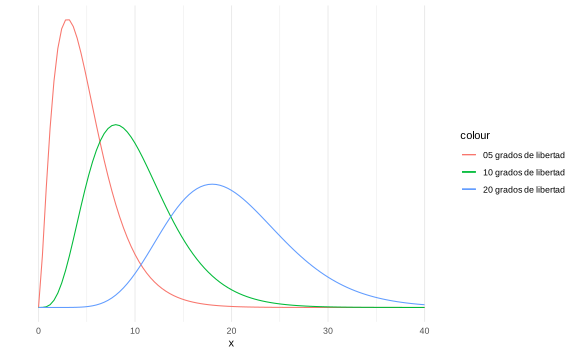
\includegraphics[width=1\linewidth]{Notas-Curso-Estadistica_files/figure-latex/unnamed-chunk-41-1} \end{center}

\hypertarget{distribuciuxf3n-t}{%
\section{\texorpdfstring{Distribución \(t\)}{Distribución t}}\label{distribuciuxf3n-t}}

\textbf{Definición}. Sea \(Y\) y \(Z\) dos variables independientes tal que \(Y\sim \chi^2_m\) y \(Z\sim N(0,1)\). Si
\[X := \dfrac Z{\sqrt{\dfrac Ym}},\]
tiene una distribución \textbf{\(t\) de Student} con \(m\) grados de libertad. Tiene como densidad
\[f_X(x) = \dfrac{\Gamma\left(\dfrac{m+1}2\right)}{\sqrt{m\pi}\Gamma\left(\dfrac m2 \right)}\left(1+\dfrac{x^2}m\right)^{-\frac{m+1}2}, \quad x\in \mathbb R.\]

\textbf{Propiedades}:

\begin{enumerate}
\def\labelenumi{\arabic{enumi}.}
\item
  \(f_X\) es simétrica.
\item
  La media de \(X\) no existe si \(m\leq 1\). Si la media existe, es 0.
\item
  Las colas de una \(t\) de Student son más pesadas que una \(N(0,1)\).
\item
  Si \(m\) es entero, los primeros \(m-1\) momentos de \(X\) existen y no hay momentos de orden superior.
\item
  Si \(m>2\), \(\text{Var}\left(X \right)=\dfrac m{m-2}\).
\item
  Si \(m=1\), \(X\sim \text{Cauchy}\).
\item
  \textbf{Ejercicio}: \(f_x(x)\xrightarrow[m\to \infty]{}\Phi(x)\) (sirve como aproximación). La discrepancia de ambas está en la cola y se disipa cuando \(m\) es grande.
\end{enumerate}

Recuerde que, por el teorema 8.3.1, \(\bar X_n\) y \(Y=\dfrac{n\hat\sigma^2}{\sigma}\) son independientes, con \(\bar X_n \sim N\left(\mu, \dfrac{\sigma^2}{n}\right)\) y \(Y\sim \chi^2_{n-1}\). Además,
\[Z = \sqrt n\dfrac{\bar X_n-\mu}{\sigma} \sim N(0,1).\]

Sea

\[T = \dfrac Z{\sqrt{\dfrac Y{n-1}}} = \dfrac{\sqrt n \dfrac{\bar X_n-\mu}{\sigma}} {\sqrt{\dfrac{\dfrac{n\hat\sigma^2}{\sigma^2}}{n-1}}} = \dfrac{\bar X_n-\mu}{\sqrt{\dfrac{\hat\sigma}{n-1}}}\]
el cual no depende de \(\sigma\).

\textbf{Teorema}. Si \(X_1,\dots, X_n \stackrel{i.i.d}{\sim} N(\mu,\sigma^2)\), defina
\[\sigma' = \bigg[\dfrac 1{n-1}\sum_{i=1}^n(X_i-\bar X_n)^2\bigg]^\frac 12.\]
Entonces
\[\dfrac{\sqrt{n}(\bar X_n-\mu)}{\sigma'} \sim t_{n-1}\]

\textbf{Nota}. \(\sigma' = \left(\dfrac n{n-1}\right)^\frac 12 \hat\sigma\) (si \(n\) es grande, \(\sigma' = \hat\sigma\)).

\emph{Prueba}. Sean
\[S_n^2=\sum_{i=1}^n(X_i-\bar X_n)^2, \quad Z = \sqrt n \dfrac{\bar X_n-\mu}{\sigma}. \]
Dado que \(Y = \dfrac{S_n^2}{\sigma^2}\sim \chi^2_{n-1}\), entonces

\begin{align*}
U = \dfrac{Z}{\sqrt{\dfrac Y{n-1}}} & = \dfrac{\dfrac{\sqrt n}\sigma (\bar X_n-\mu)}{\sqrt{\dfrac{S_n^2}{\sigma^2(n-1)}}} \\ & = \dfrac{\sqrt n (\bar X_n-\mu)}{\sqrt{\dfrac{S_n^2}{n-1}}}\\& = \dfrac{\sqrt n (\bar X_n-\mu)}{\sigma'} \sim t_{n-1}.
\end{align*}

\begin{Shaded}
\begin{Highlighting}[]
\KeywordTok{ggplot}\NormalTok{(}\DataTypeTok{data =} \KeywordTok{data.frame}\NormalTok{(}\DataTypeTok{x =} \KeywordTok{seq}\NormalTok{(}\OperatorTok{{-}}\DecValTok{5}\NormalTok{, }\DecValTok{5}\NormalTok{, }\DataTypeTok{length.out =} \DecValTok{1000}\NormalTok{)), }
    \KeywordTok{aes}\NormalTok{(x)) }\OperatorTok{+}\StringTok{ }\KeywordTok{stat\_function}\NormalTok{(}\DataTypeTok{fun =}\NormalTok{ dnorm, }\DataTypeTok{args =} \KeywordTok{list}\NormalTok{(}\DataTypeTok{mean =} \DecValTok{0}\NormalTok{, }
    \DataTypeTok{sd =} \DecValTok{1}\NormalTok{), }\KeywordTok{aes}\NormalTok{(}\DataTypeTok{color =} \StringTok{"Normal(0,1)"}\NormalTok{)) }\OperatorTok{+}\StringTok{ }\KeywordTok{stat\_function}\NormalTok{(}\DataTypeTok{fun =}\NormalTok{ dt, }
    \DataTypeTok{args =} \KeywordTok{list}\NormalTok{(}\DataTypeTok{df =} \DecValTok{1}\NormalTok{), }\KeywordTok{aes}\NormalTok{(}\DataTypeTok{color =} \StringTok{" t con 01 grados de libertad"}\NormalTok{)) }\OperatorTok{+}\StringTok{ }
\StringTok{    }\KeywordTok{stat\_function}\NormalTok{(}\DataTypeTok{fun =}\NormalTok{ dt, }\DataTypeTok{args =} \KeywordTok{list}\NormalTok{(}\DataTypeTok{df =} \DecValTok{5}\NormalTok{), }\KeywordTok{aes}\NormalTok{(}\DataTypeTok{color =} \StringTok{" t con 05 grados de libertad"}\NormalTok{)) }\OperatorTok{+}\StringTok{ }
\StringTok{    }\KeywordTok{stat\_function}\NormalTok{(}\DataTypeTok{fun =}\NormalTok{ dt, }\DataTypeTok{args =} \KeywordTok{list}\NormalTok{(}\DataTypeTok{df =} \DecValTok{10}\NormalTok{), }\KeywordTok{aes}\NormalTok{(}\DataTypeTok{color =} \StringTok{" t con 10 grados de libertad"}\NormalTok{)) }\OperatorTok{+}\StringTok{ }
\StringTok{    }\KeywordTok{ylab}\NormalTok{(}\StringTok{""}\NormalTok{) }\OperatorTok{+}\StringTok{ }\KeywordTok{scale\_y\_continuous}\NormalTok{(}\DataTypeTok{breaks =} \OtherTok{NULL}\NormalTok{) }\OperatorTok{+}\StringTok{ }
\StringTok{    }\KeywordTok{theme\_minimal}\NormalTok{()}
\end{Highlighting}
\end{Shaded}

\begin{center}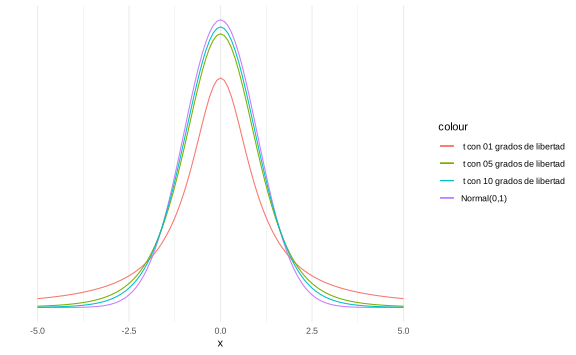
\includegraphics[width=1\linewidth]{Notas-Curso-Estadistica_files/figure-latex/unnamed-chunk-42-1} \end{center}

\hypertarget{intervalos-de-confianza}{%
\chapter{Intervalos de confianza}\label{intervalos-de-confianza}}

\hypertarget{intervalos-de-confianza-para-la-media-de-una-distribuciuxf3n-normal}{%
\section{Intervalos de confianza para la media de una distribución normal}\label{intervalos-de-confianza-para-la-media-de-una-distribuciuxf3n-normal}}

Dado \(\theta\) un parámetro en \(\mathbb{R}\) hemos estudiado procedimientos para
encontrar estadísticos \(T\in \mathbb R\) para estimarlo. La limitación que
tenemos acá es que no sabemos que tan aleatorio es \(T\). Entonces podemos
sustituir este estadístico \(T\) con otros dos estadísticos \(T_1\) y \(T_2\)
de modo que sepamos que
\begin{equation*}
T_1 \leq \theta \leq T_2
\end{equation*}

En caso que \(\theta \in \mathbb{R} ^{k}\) se puede construir un conjunto de
estadísticos \(T_1, \ldots, T_{k^\prime}\) con \(k^\prime = 2k\) tal que

\begin{equation*}
\theta \in [T_1, T_2] \times \cdots \times [T_{k^\prime-1}, T_{k^\prime}]
\end{equation*}

\hypertarget{caso-normal.}{%
\section{Caso normal.}\label{caso-normal.}}

En el caso normal, \(\bar X_n\) es un estimador puntual de \(\mu\). ¿Será posible
encontrar un estimador por intervalos?

Para efectos didácticos, vamos a empezar al revés de lo que usualmente se
acostumbra.

Defina \(U = \dfrac{\sqrt{n}(\bar X_n-\mu)}{\sigma'} \sim t_{n-1}\). Si \(c>0\),

\begin{align*} \mathbb P[-c<U<c] & = \mathbb P \bigg[ -c<\dfrac{\sqrt{n}(\bar
X_n-\mu)}{\sigma'} <c\bigg]\\ & = \mathbb P \bigg[-\dfrac{c\sigma'}{\sqrt n} <
\bar X_n - \mu <\dfrac{c\sigma'}{\sqrt n}\bigg] \\ & = \mathbb P \bigg[ \bar X_n
-\dfrac{c\sigma'}{\sqrt n} < \mu < \bar X_n + \dfrac{c\sigma'}{\sqrt n}\bigg]
\end{align*}

El intervalo

\begin{equation*}
T = \bigg[\bar X_n - \dfrac{c\sigma'}{\sqrt n},\bar X_n + \dfrac{c\sigma'}{\sqrt
n}\bigg]
\end{equation*}

es un intervalo aleatorio que ``contiene'' a \(\mu\). Si queremos restringir la
probabilidad anterior, tome \(\gamma \in (0,1)\): \[ \mathbb P(\mu\in T) = \gamma. \]

Para que se cumpla lo anterior, seleccione \(c\) tal que

\begin{align*} \gamma = \mathbb P( \mu \in T) & = F_{t_{n-1}}(c)-F_{t_{n-1}}(-c)
\\ & = F_{t_{n-1}}(c) - [1-F_{t_{n-1}}(c)]\\ & = 2F_{t_{n-1}} - 1 \end{align*}

Entonces

\[ \dfrac{\gamma+1}2 = F_{t_{n-1}}(c) \implies c = F_{t_{n-1}}^{-1}\left(\dfrac{\gamma+1}2
\right). \]

\textbf{Definición}. Si \(X\) es una variable aleatoria continua con distribución \(F\)
(monótona creciente), entonces \(x=F^{-1}(p)\) es el \textbf{cuantil} de orden \(p\) de
\(F\) (\(p\)-cuantil).

El intervalo aleatorio

\begin{equation*}
\bigg[\bar X_n -
F{t_{n-1}}^{-1}\left(\dfrac{\gamma+1}2 \right)\dfrac{\sigma'}{\sqrt n},\bar X_n
- F_{t_{n-1}}^{-1}\left(\dfrac{\gamma+1}2 \right)\dfrac{\sigma'}{\sqrt
  n}\bigg]
  \end{equation*}

contiene a \(\mu\) con probabilidad \(\gamma\).

*\textbf{Definición}. Sea \(X = (X_1,\dots,X_n)\) una muestra con parámetro \(\theta\).
Sea \(g(\theta)\) una característica de la distribución que genera la muestra. Sea \(A < B\) dos estadísticos que cumplen (\(\forall \theta\)):
\[
\mathbb P [A<g(\theta)<B]\geq \gamma.\quad
(*)
\]

Al intervalo \((A,B)\) le llamamos \textbf{intervalo de confianza con coeficiente
\(\gamma\) para \(g(\theta)\)} (intervalo de confianza al \(100\gamma\) para \(g(\theta)\)). En
el caso que \((*)\) tenga una igualdad, el intervalo es exacto.

\textbf{Nota}. Si observamos \(X\), calculamos \(A=a\), \(B=b\). Entonces \((a,b)\) es el
valor observado de un intervalo de confianza.

\textbf{Ejemplo}. Se mide la lluvia con nubes inyectadas con ``sulfato de plata'' con
\(n=26\) observaciones. Se desea hacer inferencia sobre \(\mu\), la cantidad de
lluvia media (escala logarítmica). Para \(\gamma = 0.95\), se calcula

\[
c=F^{-1}_{t_{25}}\left(\dfrac{1+\gamma}2\right) =F^{-1}_{t_{25}}(0.975) = 2.060
\]

Note que \(\frac{1+\gamma}{2}=\) \(0.975\) y el segundo valor se obtiene de
una tabla de valor de la \(t\)-student o de la expresión \texttt{qt(p\ =\ 0.975,\ df\ =\ 26-1)} = \(2.06\)

\begin{center}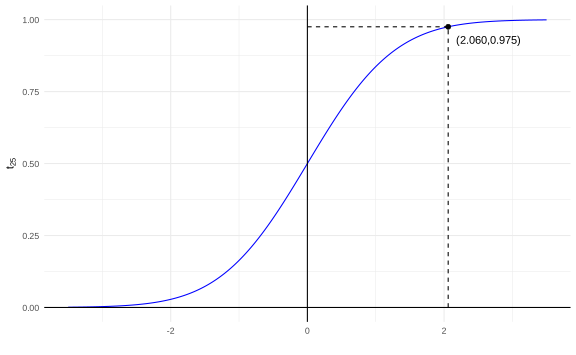
\includegraphics[width=1\linewidth]{Notas-Curso-Estadistica_files/figure-latex/unnamed-chunk-44-1} \end{center}

El intervalo de confianza para \(\mu\) al \(95\%\) es \[\bar X_n \pm
\underbrace{0.404}_{\frac{2.060}{\sqrt{26}}}\sigma'\]

Si \(\bar X_n = 5.134\) y \(\sigma' = 1.6\) el valor observado del intervalo de confianza
al \(95\%\) para \(\mu\) corresponde a

\[[5.134-0.404\cdot1.6, 5.134+0.404\cdot1.6]= [4.47,5.78]\]

\textbf{Interpretación}. El intervalo observado \([4.48,5.78]\) contiene a \(\mu\) con un
nivel de confianza del \(95%
\). Usualmente a \(\dfrac{c\sigma'}{\sqrt{n}}\) se le llama
\textbf{margen de error} (MOE).

\textbf{Interpretación gráfica}. El proceso de construir un intervalo de confianza,
quiere decir que si usted repitiera ese experimento muchas veces, el
\(100\gamma\%\) (e.g, 95\% o 99\%) de la veces, el intervalo escogido tendría el
parámetro real de la población \(\theta\).

\begin{figure}
\centering
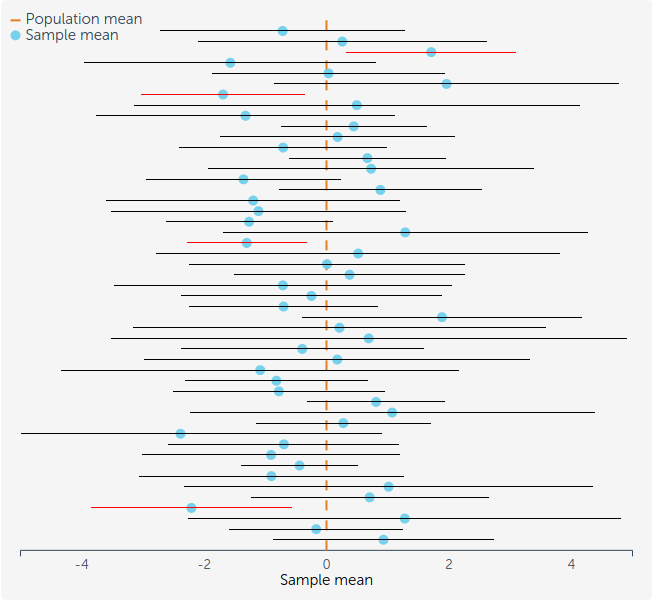
\includegraphics{./images/interpreting_confidence_intervals.png}
\caption{Ejemplo interactivo sobre intervalos de confianza. Tomado de (R Psycologist){[}\url{https://rpsychologist.com/d3/ci/}{]}}
\end{figure}

\hypertarget{intervalos-de-confianza-abiertos}{%
\section{Intervalos de confianza abiertos}\label{intervalos-de-confianza-abiertos}}

Si \(\gamma\) es el nivel de confianza dado, sea \(\gamma_1<\gamma_2\) tal que \(\gamma_2 -\gamma_1 = \gamma\). Sea \(U = \dfrac{\sqrt n}{\sigma'}(\bar X_n-\mu)\).

Si
\[
A= \bar X_n + T_{n-1}^{-1}(\gamma_1)\dfrac{\sigma'}{\sqrt n} \text{ y } B= \bar X_n +
T_{n-1}^{-1}(\gamma_2)\dfrac{\sigma'}{\sqrt n},
\]

se cumple que \((A,B)\) es un intervalo de confianza al \(100\gamma\) ya que

\[
\mathbb P[\mu \in (A,B)] = \mathbb P[T_{n-1}^{-1}(\gamma_1)<U<T_{n-1}^{-1}(\gamma_2)] =
\gamma_2-\gamma_1 = \gamma.
\]

\textbf{Definición (Intervalos de confianza abiertos)}. Bajo las condiciones
anteriores, si \(A\) es un estadístico que satisface \(\forall \theta\):

\[\mathbb P [A<g(\theta)]\geq \gamma,\]

A \(A\) se le llama \textbf{límite inferior de confianza al \(100\gamma\)} y al intervalo
\((A,\infty)\) es el \textbf{intervalo de confianza inferior al \(100\gamma\)}.

De forma análoga, si \(B\) satisface:
\[\mathbb P [g(\theta)<B]\geq \gamma,\]
a \((-\infty,B)\) se le
llama \textbf{intervalo de confianza superior} para \(g(\theta)\), con nivel \(\gamma\). Si
hay igualdad, el intervalo es exacto.

\textbf{Ejemplo}. En el caso normal, encuentra \(B\) tal que \(\mathbb P(\mu<B) = \gamma\).
Se sabe que

\[F_{t_{n-1}}(c) = \mathbb P(U>-c) = \mathbb P \left(\dfrac{\sqrt n(\mu - \bar
X_n)}{\sigma'}<c\right).\]

Entonces
\[\gamma = \mathbb P\left(\mu < \bar X_n\dfrac{\sigma'}{\sqrt n}c\right).\]

Tome \(c\) tal que
\[F_{t_{n-1}}(-c) = \gamma \implies c = -F_{t_{n-1}}(\gamma)\]

Por lo tanto
\[B = \bar X_n - \dfrac{\sigma'}{\sqrt{n}}F^{-1}_{t_{n-1}}(\gamma).\]

\hypertarget{intervalos-de-confianza-en-otros-casos}{%
\section{Intervalos de confianza en otros casos}\label{intervalos-de-confianza-en-otros-casos}}

\textbf{Ejemplo}. Tiempos de vida, \(n=3\), \(X_i\sim \text{Exp}(\theta)\).

Si \(T = \sum_{i=1}^3X_i\), \(\theta T\sim \Gamma(3,1)\).

Queremos calcular un intervalo de confianza superior para \(\theta\) al
\(100\delta\) (exacto): \(\mathbb P[\theta<B] = \gamma\).

Si \(G\) es la función de distribución de la gamma, sabemos que

\begin{equation*}
\gamma = \mathbb{P}[\theta T<G^{-1}(\gamma)] = \mathbb{P}\bigg[\theta<\dfrac{G^{-1}(\gamma)}{T}\bigg].
\end{equation*}

El límite superior es \(\dfrac{G^{-1}(\gamma)}{T}\).

\begin{Shaded}
\begin{Highlighting}[]
\NormalTok{theta \textless{}{-}}\StringTok{ }\DecValTok{2}
\NormalTok{X \textless{}{-}}\StringTok{ }\KeywordTok{rexp}\NormalTok{(}\DecValTok{3}\NormalTok{, }\DataTypeTok{rate =}\NormalTok{ theta)}
\NormalTok{T \textless{}{-}}\StringTok{ }\KeywordTok{sum}\NormalTok{(X)}
\NormalTok{G\_inv \textless{}{-}}\StringTok{ }\KeywordTok{qgamma}\NormalTok{(}\DataTypeTok{p =} \FloatTok{0.98}\NormalTok{, }\DataTypeTok{shape =} \DecValTok{3}\NormalTok{, }\DataTypeTok{rate =} \DecValTok{1}\NormalTok{)}
\end{Highlighting}
\end{Shaded}

Entonces el intervalo de confianza para este caso es

\begin{Shaded}
\begin{Highlighting}[]
\KeywordTok{c}\NormalTok{(}\DecValTok{0}\NormalTok{, G\_inv}\OperatorTok{/}\NormalTok{T)}
\end{Highlighting}
\end{Shaded}

\begin{verbatim}
## [1] 0.000000 5.702774
\end{verbatim}

\textbf{Definición}. Sea \(X = (X_1,\dots,X_n)\) una muestra de una distribución
\(F_\theta\). Sea \(V(X,\theta)\) una variable aleatoria cuya distribución no
depende de \(\theta\). Decimos que \(V\) es una \textbf{cantidad pivotal}.

Los intervalos de confianza se determinan a partir de un proceso de inversión de
la cantidad pivotal.

Encuentre \(r(v,x)\) tal que

\[r(V(X,\theta)) = g(\theta) \quad (*)\]

y \(g\) es una función cualquiera.

Del ejemplo anterior, \(V(X,\theta) = \theta T\), \[r(V(X,\theta),X) = \dfrac{V(X,\theta)}T
= g(\theta) = \theta.\]

\textbf{Teorema}. Bajo las condiciones anteriores, si \(V\) existe sea \(G\) su c.d.f. y
asume que \(G\) es continua. Asuma que \(r\) en es cierta y asuma que \(r(v,x) \nearrow\) en \(v\) para cada \(x\). Sea \(0<\gamma<1\) y \(\gamma_2>\gamma_1\) tal que \(\gamma_2-\gamma_1 = \gamma\). Entonces los extremos del intervalo de confianza para \(g(\theta)\) al
\(100\gamma\) son \[A=r(G^{-1}(\gamma_1),X), \quad B=r(G^{-1}(\gamma_2),X).\]

\textbf{Ejemplo}. \(X_1,\dots, X_n \stackrel{i.i.d}{\sim} N(\mu,\sigma^2)\). Encuentra A, B tales
que \(\mathbb P[A<\sigma^2<B] = \gamma\).

Se sabe que \[\dfrac{n\hat\sigma^2}{\sigma^2}\sim \chi^2_{n-1}.\] Tome \(V(X,\sigma^2) = \dfrac{n\hat\sigma^2}{\sigma^2}\). Entonces \[\gamma = \mathbb
P[\chi^2_{n-1,\gamma_1}<V(X,\sigma^2)<\chi^2_{n-1,\gamma_2}]\]

donde \(\gamma = \gamma_2-\gamma_1\). Tome \[r(v,X) =\dfrac{\sum(X_i -\bar X_n) ^2}{v} =
\dfrac{n\hat\sigma}{v}.\]

Invirtiendo el intervalo, \[\gamma = \mathbb P \bigg[ \underbrace{\dfrac{\sum(X_i -\bar
X_n) ^2}{\chi^2_{n-1,\gamma_2}}} _{A} <\sigma^2<\underbrace{\dfrac{\sum(X_i -\bar X_n)
^2}{\chi^2_{n-1,\gamma_1}}}_B\bigg]\]

El IC para \(\sigma^2\) al \(100\delta\) es

\[ \Bigg[ \dfrac{\sum(X_i -\bar X_n) ^2}{\chi^2_{n-1,\gamma_2}}, \dfrac{\sum(X_i -\bar X_n)
^2}{\chi^2_{n-1,\gamma_1}}\Bigg].\]

Por ejemplo

\begin{Shaded}
\begin{Highlighting}[]
\NormalTok{X \textless{}{-}}\StringTok{ }\KeywordTok{rnorm}\NormalTok{(}\DataTypeTok{n =} \DecValTok{1000}\NormalTok{, }\DecValTok{0}\NormalTok{, }\DecValTok{2}\NormalTok{)}

\NormalTok{gamma1 \textless{}{-}}\StringTok{ }\FloatTok{0.025}
\NormalTok{gamma2 \textless{}{-}}\StringTok{ }\FloatTok{0.975}

\NormalTok{gamma2 }\OperatorTok{{-}}\StringTok{ }\NormalTok{gamma1}
\end{Highlighting}
\end{Shaded}

\begin{verbatim}
## [1] 0.95
\end{verbatim}

\begin{Shaded}
\begin{Highlighting}[]
\NormalTok{(chi2\_gamma1 \textless{}{-}}\StringTok{ }\KeywordTok{qchisq}\NormalTok{(}\DataTypeTok{p =}\NormalTok{ gamma1, }\DataTypeTok{df =} \DecValTok{1000} \OperatorTok{{-}}\StringTok{ }\DecValTok{1}\NormalTok{))}
\end{Highlighting}
\end{Shaded}

\begin{verbatim}
## [1] 913.301
\end{verbatim}

\begin{Shaded}
\begin{Highlighting}[]
\NormalTok{(chi2\_gamma2 \textless{}{-}}\StringTok{ }\KeywordTok{qchisq}\NormalTok{(}\DataTypeTok{p =}\NormalTok{ gamma2, }\DataTypeTok{df =} \DecValTok{1000} \OperatorTok{{-}}\StringTok{ }\DecValTok{1}\NormalTok{))}
\end{Highlighting}
\end{Shaded}

\begin{verbatim}
## [1] 1088.487
\end{verbatim}

\begin{Shaded}
\begin{Highlighting}[]
\NormalTok{(diferencias \textless{}{-}}\StringTok{ }\KeywordTok{sum}\NormalTok{((X }\OperatorTok{{-}}\StringTok{ }\KeywordTok{mean}\NormalTok{(X))}\OperatorTok{\^{}}\DecValTok{2}\NormalTok{))}
\end{Highlighting}
\end{Shaded}

\begin{verbatim}
## [1] 4158.789
\end{verbatim}

Finalmente el intervalo es

\begin{Shaded}
\begin{Highlighting}[]
\KeywordTok{c}\NormalTok{(diferencias}\OperatorTok{/}\NormalTok{chi2\_gamma2, diferencias}\OperatorTok{/}\NormalTok{chi2\_gamma1)}
\end{Highlighting}
\end{Shaded}

\begin{verbatim}
## [1] 3.820706 4.553580
\end{verbatim}

\textbf{NOTA: Las cantidades pivotales no siempre existen. Esto ocurre principalemente
con las distribuciones discretas}

\hypertarget{intervalos-de-confianza-aproximados.}{%
\subsection{Intervalos de confianza aproximados.}\label{intervalos-de-confianza-aproximados.}}

Sean \(X_1,\dots, X_n \stackrel{i.i.d}{\sim}F_{\mu}\) donde \(\mathbb{E}[X_i] = \mu\) y
\(\text{Var}(X_i) = \sigma^2\) (conocida). Note que \[D = \mathbb P[A<\mu<B] = \mathbb P
\bigg[-z_{\frac{1+\gamma}2}<\dfrac{\sqrt n(\bar X_n-\mu)}{\sigma} <z_{\frac{1+\gamma}2}\bigg]
\stackrel{TLC}{\approx} \gamma.\]

Así, \[D \underset{n\to\infty}{\approx}
\Phi\left(z_{\frac{1+\gamma}2}\right)-\Phi\left(-z_{\frac{1+\gamma}2}\right) = \gamma.\]

\textbf{Ejercicio}. El intervalo de confianza correspondiente para \(\mu\) es

\[
\bar
X_n \pm z_{\frac{1+\gamma}2}\dfrac{\sigma}{\sqrt n}.
\]

Considere \(U = \dfrac{\bar X_n - \mu}{\sigma'/\sqrt n}\). \(U\) es pivotal, pero no
necesariamente una \(t_{n-1}\).

Considere que \((\sigma')^2 = \dfrac{n}{n-1}\hat \sigma^2\) y además \(\hat\sigma^2\) es el MLE de
\(\sigma^2\) y por lo tanto consistente.

\begin{align*}
\hat{\sigma}^2 &\xrightarrow[]{\mathbb{P}}\sigma^2 \\
((\sigma')^2 &\xrightarrow[]{\mathbb{P}}\hat{\sigma}^2).
\end{align*}

Recuerde que si \(X_n\xrightarrow[]{d}Z\) y \(Y_n\xrightarrow[]{\mathbb{P}}a\), entonces
\(X_nY_n \xrightarrow[]{d}aZ\).

Por lo tanto,
\[
\underbrace{\dfrac{\bar X_n-\mu}{\sigma/\sqrt n}}_{\xrightarrow[]{d}
N(0,1)} \cdot \underbrace{\dfrac{\sigma/\sqrt n}{\sigma'/\sqrt n}}_{\xrightarrow[]{\mathbb
P}1} \xrightarrow[]{d}N(0,1)\]

Entonces \(U\xrightarrow[]{d}N(0,1)\).

Como consecuencia

\[
\mathbb P \bigg[-z_{\frac{1+\gamma}2}<\dfrac{\bar X_n-\mu}{\sigma'/\sqrt n}
<z_{\frac{1+\gamma}2}\bigg] \stackrel{TLC}{\approx} \gamma.
\]

y el IC aproximado para \(\mu\) al \(100\gamma\)

\[\bar X_n \pm z_{\frac{1+\gamma}2}\dfrac{\sigma'}{\sqrt n}.\]

\textbf{Ejemplo}. Si \(X_1,\dots, X_n\sim \text{Poi}(\theta)\), \(\mu =\sigma^2 = \theta\). Por TLC,
\[\sqrt n\dfrac{\bar X_n-\theta}{\sqrt{\theta}}\xrightarrow[]{d}N(0,1).\] Entonces

\[
\mathbb P[|\bar X_n-\theta|<c] = \mathbb P\bigg[\dfrac{\sqrt n|\bar X_n-\theta|}{\sqrt \theta}<\dfrac{c\sqrt n}{\sqrt \theta}\bigg] \approx 2\Phi\left(\dfrac{c\sqrt n}{\sqrt \theta}\right)-1.
\]

\textbf{Explicación del fenómeno:} En este caso recuerden que \(\bar{X}_n\) es una
variable aleatoria. Lo que dice el teorema del límite central es que conforme
\(n\) es grande, la distribución de \(\bar{X}_n\) (centrada y escalada
apropiadamente) converge a una normal estándar.

\begin{Shaded}
\begin{Highlighting}[]
\NormalTok{Xbar \textless{}{-}}\StringTok{ }\KeywordTok{data.frame}\NormalTok{(}\DataTypeTok{n =} \KeywordTok{numeric}\NormalTok{(), }\DataTypeTok{Z =} \KeywordTok{numeric}\NormalTok{())}

\NormalTok{idx \textless{}{-}}\StringTok{ }\KeywordTok{rep}\NormalTok{(}\DataTypeTok{x =} \KeywordTok{c}\NormalTok{(}\DecValTok{10}\NormalTok{, }\DecValTok{2000}\NormalTok{), }\DataTypeTok{times =} \DecValTok{1000}\NormalTok{)}
\ControlFlowTok{for}\NormalTok{ (k }\ControlFlowTok{in} \DecValTok{1}\OperatorTok{:}\KeywordTok{length}\NormalTok{(idx)) \{}
\NormalTok{    muestra \textless{}{-}}\StringTok{ }\KeywordTok{rpois}\NormalTok{(}\DataTypeTok{n =}\NormalTok{ idx[k], }\DataTypeTok{lambda =} \DecValTok{5}\NormalTok{)}
\NormalTok{    Xbar[k, }\StringTok{"Z"}\NormalTok{] \textless{}{-}}\StringTok{ }\KeywordTok{sqrt}\NormalTok{(idx[k]) }\OperatorTok{*}\StringTok{ }\NormalTok{(}\KeywordTok{mean}\NormalTok{(muestra) }\OperatorTok{{-}}\StringTok{ }
\StringTok{        }\DecValTok{5}\NormalTok{)}\OperatorTok{/}\KeywordTok{sqrt}\NormalTok{(}\DecValTok{5}\NormalTok{)}
\NormalTok{    Xbar[k, }\StringTok{"n"}\NormalTok{] \textless{}{-}}\StringTok{ }\NormalTok{idx[k]}
\NormalTok{\}}



\KeywordTok{ggplot}\NormalTok{(Xbar) }\OperatorTok{+}\StringTok{ }\KeywordTok{geom\_histogram}\NormalTok{(}\DataTypeTok{mapping =} \KeywordTok{aes}\NormalTok{(}\DataTypeTok{x =}\NormalTok{ Z, }
    \DataTypeTok{y =}\NormalTok{ ..density..), }\DataTypeTok{color =} \StringTok{"white"}\NormalTok{) }\OperatorTok{+}\StringTok{ }\KeywordTok{stat\_function}\NormalTok{(}\DataTypeTok{fun =}\NormalTok{ dnorm, }
    \DataTypeTok{args =} \KeywordTok{list}\NormalTok{(}\DataTypeTok{mean =} \DecValTok{0}\NormalTok{, }\DataTypeTok{sd =} \DecValTok{1}\NormalTok{), }\DataTypeTok{color =} \StringTok{"red"}\NormalTok{) }\OperatorTok{+}\StringTok{ }
\StringTok{    }\KeywordTok{facet\_wrap}\NormalTok{(. }\OperatorTok{\textasciitilde{}}\StringTok{ }\NormalTok{n, }\DataTypeTok{scales =} \StringTok{"free"}\NormalTok{)}
\end{Highlighting}
\end{Shaded}

\begin{center}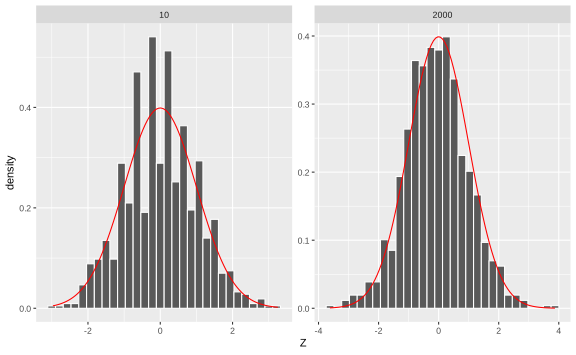
\includegraphics[width=1\linewidth]{Notas-Curso-Estadistica_files/figure-latex/unnamed-chunk-49-1} \end{center}

\hypertarget{transformaciones-estabilizadoras-de-la-varianza}{%
\subsection{Transformaciones estabilizadoras de la varianza}\label{transformaciones-estabilizadoras-de-la-varianza}}

{[}Ver página 365 del libro de texto. \}

¿Cómo transformar \(X_n\) para que tenga varianza constante? Note que en el caso
anterior se necesitó saber explícitamente el valor exacto de \(\theta\) para
hacer el ejercicio.

Por el método Delta, la varianza ``aproximada'' de \(\alpha(\bar X_n)\) es \[\left(
\dfrac{\alpha'(\mu)}{a_n}\right)^2 =\left( \dfrac{\alpha'(\mu)\sigma}{\sqrt n}\right)^2 =
\dfrac{\alpha'(\mu)^2\sigma^2(\mu)}{n}.\] Si se desea que la varianza sea constante con
respecto a \(\mu\),

\begin{align*}
\alpha'(u)^2\sigma^2(\mu) &= 1 \\
\implies \alpha'(\mu) & = \dfrac{1}{\sigma(\mu)} \quad (\sigma(\mu)>0)\\
\implies \alpha(\mu) &=
\int_{a}^{\mu} \dfrac{dx}{\sigma(x)}dx
\end{align*}

donde \(a\) es una constante arbitraria que hace la integral finita (y fácil de
calcular).

Del ejemplo anterior (Poisson), recuerde que \(\sigma ^{2} = \theta = \mu\), entonces se
podría tomar que \(\sigma(\mu) = \sqrt{\mu}\) y por lo tanto definimos

\[
\alpha(\mu) = \int_{0}^\mu\dfrac{dx}{\sqrt x} = 2\sqrt \mu
\]

Por el método Delta,\\
\[
2\bar X_n^{\frac12} \underset{n \text{ grande}}{\sim}
N\left(2\theta^{\frac 12},\dfrac1n\right)
\]

De esta manera

\[\mathbb P[|2\bar X_n^{\frac12}-2\theta^{\frac12}|<c] =\mathbb P\Bigg[\dfrac{|2\bar
X_n^{\frac12}-2\theta^{\frac12}|}{\sqrt{1/n}}<\sqrt nc\Bigg] \approx 2\Phi(\sqrt nc)-1 \]

Desarrollando, \[\mathbb P[-c+2\bar X_n^{\frac12}<2\theta^{\frac 12}<c+2\bar
X_n^{\frac12}]\approx 2\Phi(\sqrt nc)-1 \]

Se despeja \(c\) tal que \[\Phi(\sqrt n c) = \dfrac{1+\gamma}2\implies c = \dfrac 1{\sqrt
n} z_{\frac{1+\gamma}2}.\]

El intervalo para \(2\theta^{\frac 12}\) es \[\bigg[2\bar X_n^{\frac 12} -\dfrac
1{\sqrt n} z_{\frac{1+\gamma}2},2\bar X_n^{\frac 12} +\dfrac 1{\sqrt n}
z_{\frac{1+\gamma}2}\bigg]\]

\begin{Shaded}
\begin{Highlighting}[]
\KeywordTok{set.seed}\NormalTok{(}\DecValTok{42}\NormalTok{)}
\NormalTok{X \textless{}{-}}\StringTok{ }\KeywordTok{rpois}\NormalTok{(}\DataTypeTok{n =} \DecValTok{1000}\NormalTok{, }\DataTypeTok{lambda =} \DecValTok{5}\NormalTok{)}
\NormalTok{Xbar \textless{}{-}}\StringTok{ }\KeywordTok{mean}\NormalTok{(X)}
\NormalTok{z \textless{}{-}}\StringTok{ }\KeywordTok{qnorm}\NormalTok{(}\DataTypeTok{p =} \FloatTok{0.975}\NormalTok{)}

\KeywordTok{c}\NormalTok{(}\DecValTok{2} \OperatorTok{*}\StringTok{ }\KeywordTok{sqrt}\NormalTok{(Xbar) }\OperatorTok{{-}}\StringTok{ }\DecValTok{1}\OperatorTok{/}\KeywordTok{sqrt}\NormalTok{(}\DecValTok{1000}\NormalTok{) }\OperatorTok{*}\StringTok{ }\NormalTok{z, }\DecValTok{2} \OperatorTok{*}\StringTok{ }\KeywordTok{sqrt}\NormalTok{(Xbar) }\OperatorTok{+}\StringTok{ }
\StringTok{    }\DecValTok{1}\OperatorTok{/}\KeywordTok{sqrt}\NormalTok{(}\DecValTok{1000}\NormalTok{) }\OperatorTok{*}\StringTok{ }\NormalTok{z)}
\end{Highlighting}
\end{Shaded}

\begin{verbatim}
## [1] 4.371529 4.495488
\end{verbatim}

Para estimar el IC para \(\theta\), vea que si \(y=2x^{\frac12} \implies x = \dfrac{y^2}{4}\). Aplicando esta transformación al intervalo anterior, se obtiene

\[\bigg[\dfrac 14 \left(2\bar X_n^{\frac 12} -\dfrac 1{\sqrt n}
z_{\frac{1+\gamma}2}\right)^2,\dfrac 14 \left(2\bar X_n^{\frac 12} +\dfrac 1{\sqrt n}
z_{\frac{1+\gamma}2}\right)^2\bigg].\]

\begin{Shaded}
\begin{Highlighting}[]
\KeywordTok{c}\NormalTok{((}\DecValTok{1}\OperatorTok{/}\DecValTok{4}\NormalTok{) }\OperatorTok{*}\StringTok{ }\NormalTok{(}\DecValTok{2} \OperatorTok{*}\StringTok{ }\KeywordTok{sqrt}\NormalTok{(Xbar) }\OperatorTok{{-}}\StringTok{ }\DecValTok{1}\OperatorTok{/}\KeywordTok{sqrt}\NormalTok{(}\DecValTok{1000}\NormalTok{) }\OperatorTok{*}\StringTok{ }\NormalTok{z)}\OperatorTok{\^{}}\DecValTok{2}\NormalTok{, (}\DecValTok{1}\OperatorTok{/}\DecValTok{4}\NormalTok{) }\OperatorTok{*}\StringTok{ }
\StringTok{    }\NormalTok{(}\DecValTok{2} \OperatorTok{*}\StringTok{ }\KeywordTok{sqrt}\NormalTok{(Xbar) }\OperatorTok{+}\StringTok{ }\DecValTok{1}\OperatorTok{/}\KeywordTok{sqrt}\NormalTok{(}\DecValTok{1000}\NormalTok{) }\OperatorTok{*}\StringTok{ }\NormalTok{z)}\OperatorTok{\^{}}\DecValTok{2}\NormalTok{)}
\end{Highlighting}
\end{Shaded}

\begin{verbatim}
## [1] 4.777567 5.052354
\end{verbatim}

\hypertarget{estimaciuxf3n-bayesiana-bajo-normalidad}{%
\chapter{Estimación Bayesiana bajo normalidad}\label{estimaciuxf3n-bayesiana-bajo-normalidad}}

\hypertarget{precisiuxf3n-de-una-distribuciuxf3n-normal}{%
\section{Precisión de una distribución normal}\label{precisiuxf3n-de-una-distribuciuxf3n-normal}}

\textbf{Definición}. La precisión \(\tau\) de una normal se define como \(\tau = \dfrac 1{\sigma^2}\).

Sean \(X_1,\dots,X_n\sim N(\mu,\sigma^2) = N(\mu,\tau)\). Su densidad corresponde a

\[f(x|\mu,\sigma^2) = \left(\dfrac 1{2\pi\sigma^2}\right)\exp\bigg[-\dfrac1{2\sigma^2}(x-\mu)^2\bigg] = \left(\dfrac \tau{2\pi}\right)\exp\bigg[-\dfrac\tau{2}(x-\mu)^2\bigg]=f(x|\mu,\tau).\]

La verosimilitud es

\[f_n(x|\mu,\tau) = \left(\dfrac\tau{2\pi}\right)^{\frac n2}\exp\bigg[-\dfrac\tau2\sum_{i=1}^2(x_i-\mu)^2
\bigg].\]

La previa de la densidad conjunta es \([\mu,\tau|x]\propto [\mu|\tau]\cdot[\tau]\) y la posterior \([\mu,\tau|x] \propto [\mu|\tau,x]\cdot[\tau|x]\).

Las previas por seleccionar son \([\mu|\tau]\sim \text{Normal}\) y \([\tau]\sim\text{Gamma}\).

\textbf{Teorema}. Si \(X_1,\dots,X_n \overset{i.i.d}{\sim} N(\mu,\tau)\), \(\mu \in \mathbb R\), \(\tau>0\) (precisión) y \(\mu\sim N(\mu_0,\lambda_0\tau)\), \(\mu\in\mathbb R\), \(\lambda_0>0\), \(\tau\sim\Gamma(\alpha_0,\beta_0)\), \(\alpha_0,\beta_0>0\).

Entonces
\[[\mu,\tau|x] \propto [\mu|\tau,x]\cdot[\tau|x]\]
donde \([\mu|\tau,x] \sim N(\mu_1,\lambda_1\tau)\) con

\[\lambda_1 = \lambda_0+n, \quad \mu_1 = \dfrac{\lambda_0\mu_0 + n\bar x_n}{\lambda_0+n},\]
y \([\tau] \sim \Gamma(\alpha_1,\beta_1)\),
\[\alpha_1 = \alpha_0+\dfrac n2, \quad \beta_1 = \beta_0  \dfrac 12s_n^2 + \dfrac{n\lambda_0(\bar X_n-\mu_0)^2}{2(\lambda_0+n)}.\]

\emph{Prueba}.

\begin{itemize}
\tightlist
\item
  Previa:
\end{itemize}

\begin{align*}
[\mu,\tau] & \propto [\mu|\tau]\cdot[\tau]\\
& = \tau^{\frac 12}\exp\bigg[-\dfrac{\lambda_0\tau}2(\mu-\mu_0)\cdot \tau^{\alpha_0-1}e^{-\beta_0\tau}\bigg]\\
& = \tau^{\alpha_0-\frac 12}\exp\bigg[-\dfrac{\lambda_0\tau}{2}(\mu-\mu_0)^2 - \beta_0\tau\bigg]
\end{align*}

\begin{itemize}
\tightlist
\item
  Por Bayes:
\end{itemize}

\begin{align*}
[\mu,\tau|x] & \propto [\mu,\tau]\cdot[x|\mu,\tau]\\
& \propto  [\mu,\tau]\cdot\tau^{\frac 12} \exp\bigg[-\dfrac\tau 2\sum(x_i-\mu)^2\bigg]\\
& \propto \tau^{\alpha_0+\frac{n+1}2-1}\exp\bigg[-\dfrac\tau 2(\lambda_0[\mu-\mu_0]^2 + \sum(x_i-\mu)^2-\beta_0\tau\bigg]
\end{align*}

Además
\[\sum_{i=1}^n (x_i-\mu)^2 = \sum_{i=1}^n (x_i-\bar x_n + \bar x_n -\mu)^2 = s_n^2 + n(\bar x_n-\mu)^2.\]

Completando cuadrados (queda como ejercicio) se obtiene

\[n(\bar x_n -\mu)^2 + \lambda_0(\mu-\mu_0)^2 = (\lambda_0+n)(\mu-\mu_1)^2 + \dfrac{n\lambda_0(\bar x_n-\mu_0)}{\lambda_0+n}.\]

Entonces

\[\sum(x_i-\mu)^2 +\lambda_0(\mu-\mu_0)^2 = (\underbrace{\lambda_0+n}_{\lambda_1})(\mu-\mu_1) + \underbrace{s_n^2+\dfrac{n\lambda_0(\bar x_n-\mu_0)}{\lambda_0+n}}_{\beta_1}\]

Entonces

\[[\mu,\tau|x] \propto \underbrace{\tau^{\overbrace{\alpha_0+\frac n2 -1}^{\alpha_1}}\exp[-\beta_1\tau]}_{[\tau|x]} \cdot \underbrace{\tau^{\frac 12} \exp\bigg[-\dfrac{\lambda_1\tau}{2}(\mu-\mu_1)^2\bigg]}_{[\mu|\tau,x]}\]

Por lo que \([\tau|x]\sim \Gamma(\alpha_1,\beta_1)\) y \([\mu|\tau,x] \sim N(\mu_1,\lambda_1\tau)\).

\textbf{Definición} Sean \(\mu,\tau\) dos variables aleatorias. Si \(\mu|\tau \sim N(\mu_0,\lambda_0\tau)\), \(\tau\sim\Gamma(\alpha_0,\beta_0)\); decimos que
\[[\mu, \tau]\sim \text{Normal - Gamma}(\mu_0,\lambda_0,\alpha_0,\beta_0).\]

\begin{itemize}
\item
  \emph{Conclusión}: la Normal-Gamma conjuga con una verosimilitud normal.
\item
  \emph{Limitación}: \(\mu\) y \(\tau\) son independientes. Al combinar con la verosimilitud, cualquier tipo de independencia a nivel de previas se pierde.
\end{itemize}

\textbf{Ejemplo}. Concentraciones de ácido en queso \(X_1,\dots, X_n\sim N(\mu,\tau)\),
\[\mu,\tau \sim \text{Normal-Gamma}(\mu_0 = 1, \lambda_0 = 1,\alpha_0 = 1/2, \beta_0 = 1/2)\]

Los datos de este experimento son \(n = 10\), \(\bar x_n = 1.379\), \(s_n^2 = 0.9663\). Aplicando las fórmulas del teorema anterior:

\begin{itemize}
\item
  \(\mu_1 = \dfrac{1\cdot 1 + 10\cdot 1.379}{1+10} = 1.345\).
\item
  \(\lambda_1 = \lambda_0+n = 1 +10 = 11\).
\item
  \(\alpha_1 = \alpha_0 + \dfrac n2 = \dfrac 12 +\dfrac{10}2 = 5.5\).
\item
  \(\beta_1 = \dfrac 12 + \dfrac 12\cdot 0.9663 + \dfrac{10\cdot1\cdot (1.379-1)^2}{2(1+10)} = 1.0484.\)
\end{itemize}

La posterior es \[[\mu, \tau]\sim \text{Normal - Gamma}(\mu_1,\lambda_1,\alpha_1,\beta_1).\]

Calculamos

\begin{align*}
\mathbb P[\sigma>0.3|x] & = \mathbb P\bigg[\sqrt{\dfrac 1\tau} >0.3\bigg|x\bigg]\\
& = \mathbb P\bigg[\dfrac 1\tau >0.3^2\bigg|x\bigg]\\ 
& = \mathbb P\bigg[\tau >\dfrac 1{0.3^2}\bigg|x\bigg] = 0.984
\end{align*}

dado que \([\tau|x] \sim \Gamma(\alpha_1,\beta_1) = \Gamma(5.5,1.0484)\).

\hypertarget{distribuciuxf3n-marginal-de-mu}{%
\section{\texorpdfstring{Distribución marginal de \(\mu\)}{Distribución marginal de \textbackslash mu}}\label{distribuciuxf3n-marginal-de-mu}}

\textbf{Teorema}. Suponga que \([\mu,\tau]\sim \text{Normal-Gamma}(\mu_0,\lambda_0,\alpha_0,\beta_0)\). Entonces

\[\left(\dfrac{\lambda_0\alpha_0}{\beta}\right)^{\frac 12}(\mu-\mu_0)\sim t_{2\alpha_0}.\]

\emph{Prueba}. Vea que \(\mu|\tau \sim N(\mu_0,\lambda_0\tau)\). Se despeja la desviación estándar,
\[\lambda_0\tau = \dfrac 1{\sigma^2} \implies \sigma = (\lambda_0\tau)^{-\frac 12}.\]

Entonces
\[Z = \dfrac{\mu-\mu_0}{\sqrt{\lambda_0\tau}}\Bigg|\tau \sim N(0,1).\]

La densidad conjunta de \((Z,\tau)\) es
\[f(z,\tau) = \pi_2(\tau)\cdot\pi_1(z|\tau)\]

Si \(g_1(\mu|\tau)\) es la densidad de \(\mu|\tau\), por teorema de cambio de variable

\begin{align*}
f(z,\tau) & = \pi_2(\tau)\cdot \underbrace{g_1((\lambda_0\tau)^{-\frac 12}z+\mu_0|\tau)(\lambda_0\tau)^{-\frac 12}}_{\phi(z)}
= \pi_2\phi(z)
 \end{align*}

Entonces \(Z\) y \(\tau\) son independientes y \(Z\sim N(0,1)\).

Sea \(Y = 2\beta_0\tau\) y \(\tau\sim \Gamma(\alpha_0,\beta_0)\), entonces

\[Y\sim \Gamma\left(\dfrac{2\alpha_0}{2},\dfrac12 \implies Y\sim \chi^2_{2\alpha_0}\right)\]
y \(Y\) es independiente de \(Z\).

Por lo tanto,
\[U = \dfrac Z{\left( \dfrac Y{2\alpha_0}\right)^{\frac 12}}\sim t_{2\alpha_0}.\]
Observe que
\[U = \dfrac{(\lambda_0\tau)^{\frac 12}(\mu-\mu_0)}{\left( \dfrac {2\beta_0\tau}{2\alpha_0}\right)^{\frac 12}} =\left(\dfrac{\lambda_0\alpha_0}{\beta_0}\right)^{\frac 12}(\mu-\mu_0). \]

\textbf{Consecuencia}:

\[\mu =\left(\dfrac{\beta_0}{\lambda_0\alpha_0}\right)^{\frac 12} U+\mu_0,\quad U\sim t_{2\alpha_0}.\]

\textbf{Propiedades}:

\begin{itemize}
\item
  \(\mathbb E(\mu) = \mu_0 + 0 = \mu_0\).
\item
  \(\text{Var}(\mu) = \dfrac{\beta_0}{\alpha_0\lambda_0}\cdot \dfrac{\alpha_0}{\alpha_0-1} = \dfrac{\beta_0}{\lambda_0(\alpha_0-1)}\).
\end{itemize}

\textbf{Ejemplo}. \(X_1,\dots,X_{18}\) días de hospitalización en 18 centros de salud.

\[[\mu,\tau]\sim \text{Normal-Gamma}(\mu_0=200,\lambda_0=2,\alpha_0=2,\beta_0=6300).\]

Encuentre un intervalo que contenga \(\mu_1\) centrado en \(\mu_0\) tal que la probabilidad que eso pase sea \(0.95\).

\[\left(\dfrac{\alpha_0\lambda_0}{\beta_0}\right)^{\frac 12}(\mu-\mu_0) = 0.025(\mu - 200)\sim t_{2\cdot2} = t_4.\]
Entonces
\[0.95 = \mathbb P[l<0.025(\mu-200)<u] = 2F_{t_4}(u)-1 \implies u = t_{4,0.975} = 2.776.\]

Así,
\[\mathbb P[-2.776<0.025(\mu-200)<2.776]=0.95\]
y el intervalo es \([89,311]\).

Con datos: \(\bar X_n = 182.17\) y \(s_n^2 = 88678.5\). Los hiperparámetros posteriores son \(\mu_1 = 183.95\), \(\lambda_1 = 20\), \(\alpha_1 = 11\), \(\beta_1 = 50925.37\).

Resolvemos el mismo problema:

\[\left(\dfrac{\alpha_1\lambda_1}{\beta_1}\right)^{\frac 12}(\mu-\mu_0) = 0.0657(\mu - 183.95)\sim t_{2\alpha_1=22}.\]

Se busca \(u\):
\[F_{t_{22}}(u|x) = \dfrac{0.95+1}{2} \implies u = t_{22,0.975}=2.074\]
y
\[0.95 = \mathbb P[-2.074<0.0657(\mu-183.95)<2.074|x].\]
El \textbf{intervalo de credibilidad o predicción} es \([152.38,215.52]\).

Si \(X_1,\dots,X_{18}\sim N(\mu,\sigma^2)\), \(\mu,\sigma^2\) fijos y desconocidos.
\[\bar X_n+t_{17,0.975}\dfrac{\sigma'}{\sqrt {18}} \text{ al }95\%.\]
El intervalo de confianza es \([146.25,218.09]\).

\hypertarget{efecto-de-previas-no-informativas}{%
\section{Efecto de previas no informativas}\label{efecto-de-previas-no-informativas}}

Considere una \textbf{previa no informativa}: \([\mu,\tau] \propto [\mu]\cdot[\tau]\) (supuesto de independencia), con \([\mu] \propto 1\), \(\tau = \dfrac1{\sigma^2}\) y \([\sigma] \propto \dfrac{1}{\sigma}\).

Dado que \(\sigma = (\tau)^{-\frac{1}2}\), usando el teorema de cambio de variables,
\[\dfrac{d\theta}{d\tau} = -\dfrac12\tau^{-\frac32} \implies \bigg|\dfrac12\tau^{-\frac32}\bigg|f_\sigma\left(\dfrac 1{\tau^{\frac12}}\right) = \dfrac 12 \tau^{-1}.\]

Entonces \([\mu,\tau]\propto\tau^{-1}\).

\textbf{Ejercicio}. Verifique que \([\mu,\tau]\sim \text{Normal-Gamma}(\mu_0=0,\lambda_0=0,\alpha_0=-1/2,\beta_0=0)\).

Usando Bayes, \(X_1,\dots,X_n \sim N(\mu, \tau)\).

\begin{align*}
 \pi(\mu,\tau|x) \propto [\mu,\tau]\cdot[x|\mu, \tau] \\ & = \tau^{-1} (2\pi\sigma^2)^{-n/2}\exp\bigg[-\dfrac 1{2\sigma^2}\sum (X_i-\mu)^2\bigg]\\
 & \propto \tau^{-1} \tau^{n/2} \exp\bigg[-\dfrac \tau 2 s_n^2 - \dfrac{n\tau}{2}(\mu-\bar X_n)^2\bigg]\\
 & = \tau^{1/2} \exp\bigg[-\dfrac{n\tau}2 (\mu-\bar X_n)^2\bigg]\cdot \tau^{\frac{n-1}{2}-1}\exp\bigg[-\dfrac{s_n^2}{2}\tau \bigg]
 \end{align*}

Entonces

\[\mu|\tau \sim N(\bar X_n,n\tau)\]
\[\tau|x\sim \Gamma\left(\dfrac{n-1}2, \dfrac{s_n^2}{2}\right)\].

Por lo tanto,

\[\mu,\tau|x \sim \text{Normal-Gamma}(\mu_1 = \bar X_n,\lambda_1=n,\alpha_1=(n-1)/2,\beta_0=s_n^2/2).\]

\textbf{Ejemplo}. Tomando \(\bar X_n = 5.134\), \(s_n^2 = 63.96\) con una previa no informativa para \(\mu,\tau\). Entonces la posterior es Normal-Gamma con hiperparámetros: \(\mu_1 = 5.134\), \(\lambda_1 = 26\), \(\alpha = \dfrac{25}2\), \(\beta_1 = 31.98\). Queremos hacer inferencia sobre \(\mu\):

\begin{align*}
 0.95 & = \mathbb P[-t_{25,0.975}<U<t_{25,0.975}]\\
 & = \mathbb P\bigg[-t_{25,0.975}<\left(\dfrac{26\cdot 12.5}{31.98}\right)^{\frac 12}(\mu-5.134) <t_{25,0.975}\bigg]
 \end{align*}

El intervalo es \([4.488,5.78]\).

Calculemos \(\mathbb P[\mu>4|x]\). Sea \(w =\left(\dfrac{\alpha_1\lambda_1}{\beta_1}\right)^{\frac 12} = 3.188\).

\[\mathbb P[\mu>4|x] = P[w(\mu-\bar X_n)>w(4-\bar X_n)]=1-T_{t_{25}}(-3.615) = 0.9993.\]

Generalizando:

\[w = \left(\dfrac{n(n-1)/2}{s_n^2/2}\right)^{\frac 12} = \left(\dfrac{n(n-1)}{s_n^2}\right)^{\frac 12} = \left(\dfrac{n}{(\sigma')^2}\right)^{\frac 12}.\]

Entonces

\begin{align*}
\gamma & = \mathbb P\bigg[-t_{n-1,\frac{1+\gamma}{2}} < \left(\dfrac{n}{(\sigma')^2}\right)^{\frac 12}(\mu-\bar X_n)<t_{n-1,\frac{1+\gamma}{2}}\bigg] \\
& =  \mathbb P\bigg[\bar X_n-t_{n-1,\frac{1+\gamma}{2}}  \dfrac{\sigma'}{\sqrt n} < \mu < \bar X_n+t_{n-1,\frac{1+\gamma}{2}}  \dfrac{\sigma'}{\sqrt n}  \bigg].
\end{align*}

\hypertarget{estimaciuxf3n-insesgada}{%
\chapter{Estimación insesgada}\label{estimaciuxf3n-insesgada}}

\hypertarget{estimadores-insesgados}{%
\section{Estimadores insesgados}\label{estimadores-insesgados}}

\textbf{Definición}. Un estimador \(\delta(x)\) es un \textbf{estimador insesgado} de \(g(\theta)\) si \(\mathbb E_{\theta}[\delta(x)] = g(\theta)\), \(\forall \theta\). A \(\mathbb E_{\theta}[\delta(x)] - g(\theta)\) se le denomina \textbf{sesgo}.

\textbf{Ejemplo}. Si \(X_1,\dots, X_n \overset{i.i.d}{\sim} F_\theta\), \(\mu = \mathbb E[X_1]\), entonces
\[\mathbb E[\bar X_n] = \dfrac 1n \sum_{i=1}^n\mathbb E(X_i) = \mu\]
\(\bar X_n\) es estimador insesgado de \(\mu\).

\textbf{Ejemplo}. \(X_1,X_2,X_3 \overset{i.i.d}{\sim} \text{Exp}(\theta)\). El MLE de \(\theta\) es
\[\hat\theta = \dfrac 3T = \dfrac 3{\sum_{i=1}^{3}X_i}\]
¿Será \(\hat\theta\) un estimador insesgado?
\[\mathbb E[\hat\theta] = \mathbb E\bigg[\dfrac 3T\bigg]= 3\mathbb E\bigg[\dfrac 1T\bigg], \quad T\sim \Gamma(3,\theta)\]
Como
\(\dfrac 1T \sim \text{Gamma Inversa}\), se tiene que
\[\mathbb E\bigg[\dfrac 1T\bigg] = \dfrac{\theta}2 \implies \mathbb E[\hat \theta] =\dfrac{3\theta}2 \neq \theta\]
Por lo que \(\hat \theta\) es un estimador sesgado, con sesgo
\[\text{sesgo}(\hat\theta) = \dfrac{3\theta}{2} -\theta = \dfrac \theta 2.\]

Si \(U = \dfrac {2\hat\theta}{3} = \dfrac 23 \cdot \dfrac{3}{T} = \dfrac 2T\),
\[\mathbb E[U] = \dfrac 23 \mathbb E(\hat\theta) =\dfrac 23 \cdot \dfrac 32 \theta.\]
Entonces \(U\) es un estimador insesgado.

Necesitamos encontrar estimadores en donde \(\text{Var}(\delta(x))\to 0\) insesgados. ¿Cómo controlar sesgo y varianza?

\begin{align*}
\text{sesgo}^2(\delta(x))+\text{Var}(\delta(x)) & = (\mathbb E_\theta[\delta(x)]-\theta)^2 + \mathbb E[[\delta(x)-\mathbb E[\delta(x)]]^2]\\
	& =\mathbb E[ \underbrace{(\mathbb E_\theta[\delta(x)]-\theta)^2}_{A^2} + \underbrace{[\delta(x)-\mathbb E[\delta(x)]]^2}_{B^2}]\\
	& = \mathbb E[A^2+B^2 - 2(\underset{=0}{\mathbb E[\delta(x)]-\theta)(\delta(x)-\mathbb E[\delta(x)]})\\
	& =  \mathbb E[(\mathbb E[\delta(x)]-\theta - \mathbb E[\delta(x)] + \delta(x))^2]\\
	& = \mathbb E[(\delta(x)-\theta)^2] = MSE(\delta(x))
\end{align*}

\textbf{Corolario}. Si \(\delta\) tiene varianza finita, entonces

\[MSE_{\theta}(\delta(x)) =\text{sesgo}^2(\delta(x)) + \text{Var}(\delta(x)).\]

\textbf{Ejemplo}. Comparar \(\hat\theta\) y \(\delta(x) =\dfrac 2T\) en términos del MSE.

Dado que \(\text{Var}\left(\dfrac 1T\right) = \dfrac{\theta^2}4\), se tiene

\begin{itemize}
\item
  \(MSE(\delta(x)) = \text{Var}\left(\dfrac 2T\right) = 4\dfrac{\theta^2}4 = \theta^2\).
\item
  \(MSE(\hat\theta) = (\text{sesgo}(\hat\theta))^2+\text{Var}\left(\dfrac 3T\right) = \dfrac{\theta^2}{4}+\dfrac{9\theta^2}{4} = \dfrac{5\theta}{2}\).
\end{itemize}

\(\delta(x)\) es mejor estimador en términos de MSE que el \(\hat\theta\).

\hypertarget{estimador-insesgado-de-la-varianza}{%
\section{Estimador insesgado de la varianza}\label{estimador-insesgado-de-la-varianza}}

\textbf{Teorema}. Si \(X_1,\dots, X_n \sim F_{\theta}\) con varianza finita y \(g(\theta) = \text{Var}(X_1)\) entonces
\[\hat\sigma_1^2 = \dfrac{1}{n-1}\sum(X_i-\bar X_n)^2\]
es un estimador insesgado de \(\sigma^2\).

\emph{Prueba}. Considere que

\[ \sum (X_i-\mu)^2 = s_n^2 + n(\bar X_n-\mu)^2 \]
Entonces

\[\mathbb E[\hat\sigma_0^2] = \mathbb E \bigg[ \dfrac {s_n^2}n \bigg] =  \mathbb E \bigg[ \dfrac 1n \sum(X_i-\mu)^2\bigg] - \mathbb E[(\bar X_n-\mu)^2] = \sigma^2-\dfrac{\sigma^2}n = \left(\dfrac{n-1}n\right)\sigma^2.\]

Para que \(\hat\sigma_0^2\) sea insesgado,
\[\mathbb E \bigg[\dfrac n{n-1}\hat\sigma_0^2\bigg] = \mathbb E[\hat\sigma_1] = \sigma^2.\]

Entonces \(\hat\sigma_1\) es estimador insesgado de \(\sigma^2\).

\textbf{Ejemplo}. Sean \(X_1,\dots,X_n \overset{i.i.d}{\sim}\text{Poi}(\theta)\). \(\mathbb E(X_i) = \text{Var}(X_i) = \theta\). Estimadores insesgados de \(\theta\) son:

\begin{enumerate}
\def\labelenumi{\arabic{enumi})}
\item
  \(\bar X_n\).
\item
  \(\hat \sigma_1^2\).
\item
  Si \(\alpha \in (0,1)\), \(T = \alpha\bar X_n + (1-\alpha)\hat\sigma_1^2\) también es un estimador insesgado (corrige otros problemas).
\end{enumerate}

\textbf{Ejemplo}. (Normal) ¿Cuál estimador tiene menor MSE, \(\hat\sigma^2_0\) o \(\hat\sigma^2_1\)?

Defina \(T_c = cs_n^2\). Si \(c = 1/n\), \(T_c = \hat\sigma_0\) y si \(c = 1/(n-1)\), \(T_c = \hat\sigma_1\). De esta manera,

\[MSE_{\sigma^2}(T_c) = \mathbb E[(T_c-\sigma^2)^2] =(\mathbb E(T_c)-\sigma^2)^2+\text{Var}(T_c).\]

\begin{itemize}
\item
  \(\mathbb E[T_c] = c\mathbb E[s_n^2] = c(n-1)\mathbb E\bigg[\dfrac{s_n^2}{n-1}\bigg] = c(n-1)\sigma^2\).
\item
  \(\text{Var}(T_c) = c^2\text{Var}(s_n) = c^2\text{Var}\Bigg(\sigma^2\underbrace{\sum\dfrac{(X_i-\bar X_n)}{\sigma^2}}_{\sim\chi^2_{n-1}}\Bigg) = 2c^2\sigma^4(n-1)\).
\end{itemize}

Entonces

\[MSE_{\sigma^2}(T_c) = [c(n-1)\sigma^2-\sigma^2]^2+2c^2\sigma^4(n-1) = [[c(n-1)-1]^2+2c^2(n-1)]\sigma^4.\]

Optimizando,

\[\min_c MSE (T_c) = \min_c[(n^2-1)c^2-2(n-1)c+1],\]

se encuentra que \(\hat c = \dfrac 1{n+1}\). Así, \(T_{\hat c} = \dfrac{s_n^2}{n+1}\) es el mejor estimador de \(\sigma^2\) en el sentido de MSE.

\textbf{Ejercicio}. Compare \(\hat\sigma_0^2\) y \(\hat\sigma_1^2\).

\hypertarget{informaciuxf3n-de-fisher}{%
\section{Información de Fisher}\label{informaciuxf3n-de-fisher}}

¿Cómo cuantificar la información de un estadístico?

Sea \(X\sim f(x|\theta)\), \(\theta \in \Omega \subset \mathbb R\) parámetro fijo.

\begin{itemize}
\item
  \emph{Supuesto 1}: para cada \(x \in \mathcal X\) (espacio muestral de \(X\)) \(f(x|\theta)> 0\) \(\forall \theta \in \Omega\).
\item
  \emph{Restricción}: la imagen de la variable aleatoria no puede depender de \(\theta\).
\end{itemize}

\textbf{Ejemplo}. \(\text{Unif}[0,\theta]\), \(f(x|\theta) = 1_{(0,\theta)}(x)\). No aplica el supuesto, ya que si \(x>\theta\), \(f(x|\theta) = 0\).

\textbf{Definición}. Se define la \textbf{función Score}:

\[\lambda(x|\theta):=\ln f(x|\theta)\]

cuyas derivadas son

\[\lambda'(x|\theta) = \dfrac \partial{\partial \theta}\ln f(x|\theta)\]
\[\lambda''(x|\theta) = \dfrac {\partial^2}{\partial \theta^2}\ln f(x|\theta)\]

\begin{itemize}
\tightlist
\item
  \emph{Supuesto 2}: \(f(x|\theta)\) es dos veces diferenciable.
\end{itemize}

\textbf{Definición}. Si \(X\) y \(f(x|\theta)\) satisfacen los supuestos anteriores, la \textbf{información de Fisher} (\(I(\theta)\)) de \(X\) es
\[I(\theta): =\mathbb E[(\lambda'(x|\theta))^2]\]
donde la esperanza es integral o suma, dependiendo de \(X\).

\textbf{Teorema}. Bajo las condiciones anteriores, y suponiendo que las dos derivadas de \(\int_{\mathcal X}f(x|\theta)dx\) con respecto a \(\theta\) (\emph{Supuesto 3}) se pueden calcular al intercambiar el orden de integración y derivación. Entonces

\[I(\theta) = -\mathbb E_{\theta}[\lambda''(x|\theta)] = \text{Var}[\lambda'(x|\theta)].\]

\emph{Prueba}:

\begin{align*}
\mathbb E[\lambda'(x|\theta)] & \int_{\mathcal X}\lambda'(x|\theta)f(x|\theta)dx\\
& = \int_{\mathcal X} \dfrac{f'(x|\theta)}{f(x|\theta)}f(x|\theta)dx\\
& =  \int_{\mathcal X}f'(x|\theta)dx\\
& = \dfrac d{d\theta}\int_{\mathcal X}f(x|\theta)dx \quad \text{por el supuesto}\\
& = \dfrac d{d\theta}1 = 0
\end{align*}

En consecuencia,
\[\text{Var}(\lambda'(x|\theta)) = \mathbb E[(\lambda'(x|\theta))^2]-0 = I(\theta).\]

Además,
\[\lambda''(x|\theta)= \left(\dfrac{f'(x|\theta)}{f(x|\theta)}\right)' = \dfrac{f(x|\theta)f''(x|\theta)-f'(x|\theta)^2}{f^2(x|\theta)} =\dfrac{f''(x|\theta)}{f(x|\theta)} - (\lambda'(x|\theta))^2 \]

Note que

\begin{align*}
\mathbb E\bigg[\dfrac{f''(x|\theta)}{f(x|\theta)} \bigg] & = \int_{\mathcal X}\dfrac{f''(x|\theta)}{f(x|\theta)} f(x|\theta)dx \\
&=\dfrac{d}{d\theta}\bigg[\dfrac{d}{d\theta}\int_{\mathcal X}f(x|\theta)dx\bigg]\\
& = \dfrac{d}{d\theta}\bigg[\dfrac{d}{d\theta}1\bigg] = 0
\end{align*}

Entonces,
\[\mathbb E[\lambda''(x|\theta)] =\mathbb E\bigg[\dfrac{f''(x|\theta)}{f(x|\theta)} \bigg] - \mathbb E[(\lambda'(x|\theta))^2] = -I(\theta). \]

Se concluye, además, que \(\lambda'(x|\theta)\) es centrada y su varianza es \(I(\theta)\).

\textbf{Ejemplo}. \(X\sim \text{Ber}(p)\).

\begin{itemize}
\item
  \(f(x|p) = p^x(1-p)^{1-x}\), \(x=0,1\) satisface supuesto 1.
\item
  \(\displaystyle\int_{\mathcal X}f(x|p)dx \;``=" f(0|p)+f(1|p)\) satisface el supuesto 3.
\end{itemize}

Entonces,

\begin{itemize}
\item
  \(\lambda(x|p) = \ln[p^x(1-p)^x] = x\ln p + (1-x)\ln(1-p)\).
\item
  \(\lambda'(x|p) = \dfrac xp-\dfrac{1-x}{1-p}\).
\item
  \(\lambda''(x|p) = -\dfrac x{p^2}-\dfrac{1-x}{(1-p)^2}\).
\end{itemize}

De esta manera,
\[I(p) = \mathbb E\bigg[\dfrac xp + \dfrac{1-x}{(1-p)^2}\bigg] = \dfrac p{p^2}+\dfrac{1-p}{(1-p)^2} = \dfrac 1{p(1-p)} = \dfrac 1{\text{Var}(X)}.\]

\textbf{Ejemplo}. \(X\sim N(\mu,\sigma^2)\), \(\mu\) desconocida, \(\sigma^2\) conocida.
\[f(x|\mu) = \dfrac{1}{\sqrt{2\pi\sigma^2}}\exp\left(-\dfrac 1{2\sigma^2}(x-\mu)^2\right)\]

Vea que
\begin{align*}
\dfrac d{du}\int_{\mathbb R} f(x|\mu)dx & = \int_{\mathbb R}f'(x|\mu)dx\\
& = \int_{\mathbb R} -\dfrac 1{\sqrt{2\pi\sigma^2}}\dfrac {2(x-\mu)^2}{2\sigma^2} dx\\
& = -\dfrac 1\sigma \underbrace{\int_{\mathbb R}\dfrac{u}{\sqrt{2\pi}}e^{-\frac{u}2}du}_{\mathbb E[N(0,1)]} = 0 \quad \text{usando el cambio de variable } \dfrac{x-\mu}\sigma
\end{align*}

por lo que cumple el tercer supuesto.

Entonces

\begin{itemize}
\item
  \(\lambda(x|\mu) = \dfrac 12 \ln (2\pi\sigma^2)-\dfrac 1{2\sigma^2}(x-\mu)^2\).
\item
  \(\lambda'(x|\mu) = \dfrac 1{2\sigma^2}2(x-\mu) = \dfrac{x-\mu}{\sigma^2}\).
\item
  \(\lambda''(x-\mu) = -\dfrac 1{\sigma^2}\).
\end{itemize}

Por lo que

\[I(\mu) = -\mathbb E[\lambda''(x|\mu)] = \dfrac{1}{\text{Var}(X)}\]

\textbf{Definición}. Suponga que \(X = (X_1,\dots,X_n)\) muestra de \(f(x|\theta)\) donde \(f\) satisface las condiciones anteriores. Defina \(\lambda_n = \ln f_n(x|\theta)\). La información de Fisher de \(X\) es

\[I_n(\theta) = \mathbb E[(\lambda'(x|\theta))^2] = - \mathbb E[\lambda''_n(x|\theta)].\]

\textbf{Nota}. Observe que
\[\lambda_n(x|\theta) = \ln f_n(x|\theta) = \sum_{i=1}^{n} \lambda(X_i|\theta)\]
lo que implica que
\[\lambda''_n(x|\theta) = \sum_{i=1}^n(X_i|\theta).\]
De esta forma,
\[I_n(\theta) = -\mathbb E[\lambda''(x|\theta)] = - \sum_{i=1}^n\mathbb E[\lambda''(X_i|\theta)] = nI(\theta).\]

\textbf{Ejemplo}. Clientes que entran a una tienda. Este se modela a partir de un proceso de Poisson. El tiempo de llegada entre cada cliente es independiente y se distribuye como \(\text{Exp}(\theta)\). Sea \(X\) el tiempo de arribo total de \(n\) clientes (\(n\)) fijo:
\[X\sim \sum_{i=1}^{n}\text{Exp}(\theta) = \Gamma(n,\theta) .\]

Así mismo, sea \(Y\) el número de clientes hasta el tiempo \(t\):
\[Y\sim \text{Poi}(\theta t)\]

¿Cuál variable contiene más información de \(\theta\)?

Para \(Y\),

\begin{itemize}
\item
  \(f(y|\theta) = e^{-t\theta}\dfrac{(t\theta)^y}{y!}\).
\item
  \(\lambda(y|\theta) = t\theta + y\ln (t\theta) - \ln y!\).
\item
  \(\lambda'(y|\theta) = -t+\dfrac{ty}{t\theta}.\)
\item
  \(\lambda''(y|\theta) = -\dfrac y{\theta^2}\).
\end{itemize}

Entonces,
\[I_Y(\theta) =-\mathbb E[ \lambda''(y|\theta)] = \dfrac{\mathbb E[Y]}{\theta^2} = \dfrac{t}\theta.\]

Como ejercicio, verifique que \(I_X(\theta) = \dfrac n{\theta^2}\).

Ambas variables tienen la misma información si

\[I_Y(\theta) = I_X(\theta) \implies \dfrac t\theta = \dfrac n{\theta^2} \implies n = t\theta.\]

\hypertarget{desigualdad-de-cramer-rao}{%
\section{Desigualdad de Cramer-Rao}\label{desigualdad-de-cramer-rao}}

\textbf{Teorema}. Si \(X = (X_1,\dots, X_n)\) muestra de \(f(x|\theta)\). Todos los supuestos anteriores son válidos para \(f\). Sea \(T = r(X)\) un estadístico con varianza finita. Sea \(m(\theta) = \mathbb E_{\theta}[T]\) y asuma que \(m\) es diferenciable. Entonces:
\[\text{Var}_\theta(T)\geq \dfrac{[m'(\theta)]^2}{I_n(\theta)} =\dfrac{[m'(\theta)]^2}{nI(\theta)} .\]

La igualdad se da si y solo si existen funciones \(u(\theta)\) y \(v(\theta)\) que solo dependen de \(\theta\) tales que
\[T = u(\theta)\lambda_n'(x|\theta) + v(\theta).\]

\emph{Prueba}. Para el caso univariado:
\[\int_{\mathcal X}f'(x|\theta)dx = 0.\]

Para el caso multivariado:

\begin{align*}
\int_{\mathcal X^n}f'_n(x|\theta)dx_1\cdots dx_n & =\int_{\mathcal X^n}[f(x1|\theta)\cdots f(x_n|\theta)]'dx_1\cdots dx_n \\
& \dfrac d{d\theta} \int_{\mathcal X^n}f(x1|\theta)\cdots f(x_n|\theta)dx_1\cdots dx_n = 0.
\end{align*}

Entonces

\[\mathbb E[\lambda_n'(X|\theta)] = \int_{\mathcal X^n}\dfrac{f'_n(x|\theta)}{f(x|\theta)}dx_1\cdots dx_n = 0\]

Por lo tanto,

\begin{align*}
\text{Cov}[T,\lambda_n'(X|\theta)] & = \mathbb E [T\lambda_n'(X|\theta)] - \mathbb E[T]\cdot 0\\
& =\int_{\mathcal X^n}r(x)\dfrac{f'_n(x|\theta)}{f_n(x|\theta)}f_n(x|\theta)dx_1\cdots dx_n\\
& =  \dfrac d{d\theta}\int_{\mathcal X^n}r(x)f_n(x|\theta)dx_1\cdots dx_n\\
& = \dfrac{d}{d\theta}\mathbb E_\theta[r(X)] = \dfrac{d}{d\theta}E_\theta[T] = m'(\theta)
\end{align*}

Considere el coeficiente de correlación
\[\rho = \dfrac{\text{Cov}[T,\lambda_n'(X|\theta)] }{\sqrt{\text{Var}(T)}\sqrt{\text{Var}(\lambda_n'(X|\theta))}}.\]

Dado que \(|p|\leq 1 \implies \rho^2 \leq 1\), se tiene que

\[\text{Cov}[T,\lambda_n'(X|\theta)]^2 \leq \sqrt{\text{Var}(T)}\sqrt{\text{Var}(\lambda_n'(X|\theta))} \implies [m'(\theta)]^2 \leq \text{Var}(T) I_n(\theta). \]
Entonces \(\text{Var}(T)\geq \dfrac{[m'(\theta)]^2 }{I_n(\theta)}\).

\textbf{Caso particular}. Si \(T\) es un estimador insesgado de \(\theta\), entonces \(\text{Var}_\theta(T)\geq \dfrac{1 }{I_n(\theta)}\).

\textbf{Ejemplo}. \(X_1,\dots, X_n \sim \text{Exp}(\beta)\), \(n>2\).

\begin{itemize}
\item
  \(f(x|\beta) = \beta e^{-\beta x}\), \(x>0\).
\item
  \(\lambda(x|\beta) = \ln f(x|\beta) = \ln \beta -\beta x\).
\item
  \(\lambda'(x|\beta) = \dfrac 1\beta -x.\)
\item
  \(\lambda'' = -\dfrac 1{\beta^2}\).
\end{itemize}

Vea que
\[1 = \int_{0}^\infty \beta e^{-\beta x}dx = \lim_{u\to \infty}F(u) = \lim_{u\to \infty}[1-e^{-\beta u}]\]

y el supuesto 3 se puede verificar por la diferenciabilidad de \(1-e^{-\beta u}\).

Así,
\[I(\beta) = -\mathbb E[\lambda''(x|\beta)] = \dfrac 1{\beta^2}, \quad I_n(\beta) = \dfrac{n}{\beta^2}.\]

Considere el estadístico \(T = \dfrac{n-1}{\sum_{i=1}^n X_i}\) es un estimador insesgado de \(\beta\). La varianza de \(T\) es \(\dfrac{\beta^2}{n-2}\).

La cota de Cramer Rao, si \(T\) es insesgado, es

\[\dfrac 1{I_n(\beta)} = \dfrac{\beta^2}{n},\]

por lo que \(T\) no satisface la cota de Cramer Rao.

Ahora, estime \(\theta = \dfrac 1\beta = m(\beta)\). Un estimador insesgado de \(\theta\) es \(T =\bar X_n\):

\[\mathbb E[\bar X_n] = \mathbb E
[X_1] = \dfrac 1\beta  = \theta, \quad \text{Var}(\bar X_n) = \dfrac{\text{Var}(\bar X_1) }{n} = \dfrac 1{n\beta^2}.\]

La cota de Cramer es

\[\dfrac{(m'(\beta))^2}{I_n(\beta)} = \dfrac{(-1/\beta^2)^2}{n/\beta^2} = \dfrac{\beta^2}{n\beta^4} = \dfrac{1}{n\beta^2}.\]

\(\bar X_n\) satisface la cota de Cramer-Rao y además
\[\lambda'(X|\beta) = \dfrac n\beta - n\bar X_n =\dfrac n\beta - nT \implies T = \underbrace{-\dfrac 1n}_{u(\beta)}\lambda_n'(X|\beta)+ \underbrace{\dfrac 1\beta}_{v(\beta)}. \]

\hypertarget{estimadores-eficientes}{%
\section{Estimadores eficientes}\label{estimadores-eficientes}}

\textbf{Definición}. \(T\) es un estimador eficiente de su esperanza \(m(\theta)\) si su varianza es la cota de CR.

\textbf{Ejemplo}. \(X_1,\dots, X_n\sim \text{Poi}(\theta)\). \(\bar X_n\) es un estimador eficiente.

\begin{itemize}
\item
  Verosimilitud: \(f_n(X|\theta) = e ^{n\theta}\dfrac{\theta^{n\bar X_n}}{\prod X_i!}\).
\item
  \(\lambda_n(X|\theta) = -n\theta + n\bar X_n \ln \theta - \ln \prod X_i!\).
\item
  \(\lambda'_n(X|\theta) = -n+\dfrac{c\bar X_n}{\theta}\).
\item
  \(\lambda_n''(X) = -\dfrac{n\bar X_n}{\theta^2}\).
\end{itemize}

Entonces
\[\dfrac{n}{\theta^2}\mathbb E[\bar X_n] = \dfrac n{\theta}.\]

La cota de CR es \(\dfrac \theta n\), pero
\[\text{Var}(\bar X_n) = \dfrac{\text{Var}(X_1)}{m} = \dfrac \theta n.\]
Por lo que \(\bar X_n\) es eficiente.

Los otros candidatos para estimar \(\theta\)
\[\sigma_1^2=\dfrac 1{n-1}s_n^2 = \dfrac 1{n-1}\sum (X_i-\bar X_n)^2,\]
y
\[\alpha \bar X_n + (1-\alpha)\hat\sigma^2_1\]
no son lineales con respecto a \(\lambda'(X|\theta)\) por lo que tienen mayor varianza que \(\bar X_n\).

\hypertarget{comportamiento-asintuxf3tico-del-mle}{%
\section{Comportamiento asintótico del MLE}\label{comportamiento-asintuxf3tico-del-mle}}

\textbf{Teorema}. Bajo las condiciones anteriores y si \(T\) es un estimador eficiente de \(m'(\theta)\) y \(m'(\theta) \neq 0\), entonces
\[\dfrac 1{\sqrt{CR}}[T-m(\theta)]\xrightarrow{d}N(0,1)\]

\emph{Prueba}. Recuerde que \(\lambda'_n(X|\theta) = \sum_{i=1}^n\lambda'(X_i|\theta)\). Como \(X\) es una muestra, \(\lambda'(X_i|\theta)\) son i.i.d, y

\[\mathbb E[\lambda'(X_i|\theta)] = 0, \quad \text{Var}(\lambda'(X_i|\theta)) = I(\theta).\]

Como \(T\) es estimador eficiente de \(m(\theta)\),
\[\mathbb E[T] = m(\theta), \quad \text{Var}(T) = \dfrac{(m'(\theta))^2}{nI(\theta)}\]

y existen \(u(\theta)\) y \(v(\theta)\) tal que

\[T = v(\theta \lambda'(X|\theta)) + v(\theta).\]

\begin{itemize}
\item
  \(\mathbb E [T]= u(\theta)\mathbb E[\lambda'(X|\theta)] + v(\theta) \implies v(\theta) = m(\theta)\).
\item
  \(\text{Var}(T) = u^2(\theta)I_n(\theta) \implies v(\theta) = \dfrac{m'(\theta)}{nI(\theta)}\).
\end{itemize}

Entonces \(T = \dfrac{m'(\theta)}{nI(\theta)}\lambda'(X|\theta) + m(\theta)\). Por lo tanto,

\[\bigg[\dfrac{nI(\theta)}{m'(\theta)^2}\bigg]^{\frac 12}[T-m(\theta)] = \bigg[\dfrac 1 {nI(\theta)}\bigg]^{\frac 12}\lambda'_n(x|\theta) \xrightarrow[n\to\infty]{} N(0,1).\]

\textbf{Teorema}. Suponga que el MLE \(\hat \theta_n\) se obtiene al resolver \(\lambda'(x|\theta) = 0\). Además, \(\lambda''(x|\theta)\) y \(\lambda'''(x|\theta)\) existen y las condiciones anteriores son ciertas.

\[[nI(\theta)]^{1/2}(\hat\theta-\theta) \to N(0,1).\]

\textbf{Ejemplo}. \(X_1,\dots, X_n \sim N(0,\sigma^2)\), \(\sigma\) desconocida. \(\hat\sigma = \bigg[\dfrac 1n s_n^2\bigg]^{1/2}\) es MLE de \(\sigma\) y \(I(\sigma) = \dfrac 2{\sigma^2}\).
Usando el teorema,
\[\sqrt{\dfrac{2n}{\sigma^2}}\underset{n\to\infty}{\sim} N\left(\sigma,\dfrac{\sigma^2}{2n}\right).\]

Verifique que
\[\hat\sigma_n\pm z_{\frac{1+\gamma}{2}}\sqrt{\dfrac{\sigma^2}{2n}}\]
es un intervalo de confianza para \(\sigma\).

\textbf{Consecuencia en estimación bayesiana}. La previa de \(\theta\) es positiva y diferenciable con respecto a \(\theta\). Bajo todas las condiciones anteriores:
\[\theta|X\underset{n\to\infty}{\sim} N\left(\hat\theta_n,\dfrac 1{nI(\hat\theta_n)}\right).\]

\textbf{Nota}: un IC para \(\theta\) en este caso tiene un error estándar que depende del MLE.

\hypertarget{pruebas-de-hipuxf3tesis}{%
\chapter{Pruebas de hipótesis}\label{pruebas-de-hipuxf3tesis}}

\hypertarget{pruebas-de-hipuxf3tesis-1}{%
\section{Pruebas de hipótesis}\label{pruebas-de-hipuxf3tesis-1}}

Recordando el ejemplo de las nubes rociadas con químicos en donde log-lluvia \(\sim N(\mu,\sigma^2)\), \(\mu,\sigma\) desconocidos.

\textbf{Hipótesis}: \(\mu>4\) (nace a partir de una pregunta), es decir, si \(\theta = (\mu,\sigma^2)\), ¿\(\theta\in\{(\mu,\sigma^2): \mu>4\}\)?

Para el caso bayesiano, ya calculamos \(\mathbb P[\mu>4|X]\). ¿Cómo resolverlo en el caso frecuentista?

Suponga que \(\Omega = \Omega_0 \cup\Omega_1\) conjuntos disjuntos tales que
\begin{align*}
H_0 :  \text{hipótesis en donde }\theta \in \Omega_0.\\
H_1 : \text{hipótesis en donde }\theta \in \Omega_1.\\
\end{align*}

\textbf{Objetivo}. Decidir si \(H_0\) o \(H_1\) es cierto, con los datos disponibles (problema de pruebas de hipótesis).

\textbf{Definición}. \(H_0:\) hipótesis nula. \(H_1:\) hipótesis alternativa. Una vez que se ha realizado una prueba de hipótesis si afirmamos \(\theta \in \Omega_1\) decimos que \emph{rechazamos} \(H_0\). Si \(\theta \in \Omega_0\), decimos que \emph{no rechazamos} \(H_0\).

Suponga que \(X_1,\dots, X_n\sim f(x|\theta)\), \(\theta \in \Omega\), \(\Omega = \Omega_0 \cup\Omega_1\) y queremos probar la hipótesis \(H_0: \theta \in \Omega_0\), \(H_1: \theta \in \Omega_1\).

\textbf{Definición} (\(i = 0,1\))

\begin{enumerate}
\def\labelenumi{\arabic{enumi})}
\item
  Si \(\Omega_i\) tiene solamente un valor de \(\theta\), \(H_i\) es una \textbf{hipótesis simple}.
\item
  Si \(\Omega_i\) tiene más de un valor de \(\theta\), \(H_i\) es una \textbf{hipótesis compuesta}.
\item
  \textbf{Hipótesis compuestas de una cola}. Si \(\Omega_0 = (-\infty,\theta_0]\), \(H_0: \theta\geq \theta_0\), \(H_1: \theta >\theta_0\). Si \(\Omega_0 = [\theta_0,+\infty)\), \(H_0: \theta\leq \theta_0\), \(H_1: \theta<\theta_0\).
\item
  Si \(H_1: \theta \ne \theta_0\) y \(H_0: \theta = \theta_0\) es una \textbf{hipótesis de 2 colas}.
\end{enumerate}

\hypertarget{regiones-cruxedticas-y-estaduxedsticas-de-prueba}{%
\section{Regiones críticas y estadísticas de prueba}\label{regiones-cruxedticas-y-estaduxedsticas-de-prueba}}

\textbf{Ejemplo}. Si \(X_1,\dots, X_n \sim N(\mu,\sigma^2)\), \(\mu\) desconocido, \(\sigma^2\) conocido.

Queremos probar \(H_0: \mu = \mu_0\) vs \(H_1: \mu\neq \mu_0\). La lógica es: rechazamos \(H_0\) si \(\mu\) está ``muy alejado'' de \(\mu_0\).

Seleccione un número \(c\) tal que se rechaza \(H_0\) si \(|\bar X_n -\mu_0|>c\). En general, suponga que queremos probar las hipótesis \(H_0: \theta \in \Omega_0\) vs \(H_1: \theta\in \Omega_1\).

En general, supónga que queremos probar las hipótesis \(H_0: \theta \in \Omega_0\) vs \(H_1: \theta \in \Omega_1\).

Cuando tenemos una muestra \(X_1,\dots,X_n \sim f(x|\theta)\). Sea \(S_0\subset \mathcal X\): conjunto en donde no se rechaza \(H_0\) y \(S_1\subset \mathcal X\): conjunto en donde se rechaza \(H_0\).

A \(S_1\) se le llama \textbf{región crítica} de la prueba de hipótesis.

\textbf{Nota}. En la mayoría de los casos, la región crítica se define en términos de un estadístico \(T = r(x)\).

\textbf{Definición}. Sea \$ X\$ una muestra aleatoria con distribución \(f(x|\theta)\) y \(T=r(X)\) un estadístico y \(R\subset \mathbb R\). Suponga que se puede verificar las hipótesis al afirmar ``rechazamos \(H_0\) si \(T\in R\)'', entonces \(T\) es un \textbf{estadístico} de prueba y \(R\) es la \textbf{región de rechazo} de la prueba.

\textbf{Ejemplo}. En el caso en que se rechaza \(H_0\) si \(|\bar X_n|>c\), \(T = |\bar X_n-\mu_0|\) estadístico de prueba y \((c,\infty)\) es la región de rechazo.

\hypertarget{funciuxf3n-de-potencia-y-tipos-de-error}{%
\section{Función de potencia y tipos de error}\label{funciuxf3n-de-potencia-y-tipos-de-error}}

Sea \(\delta\) un procedimiento de prueba (basado en una región crítica o en un estadístico de prueba). Sea \(\pi(\theta|\delta)\) (\textbf{función de potencia}) la probabilidad de que se rechace \(H_0\) a través de \(\delta\) para \(\theta\in \Omega\).

Si \(S_1\) es la región crítica de \(\delta\) entonces \(\pi(\theta|\delta) = \mathbb P(X\in S_1|\theta)\) para \(\theta\in\Omega\).

Si \(\delta\) se describe a través de un estadístico de prueba \(T\) con región de rechazo \(R\), entonces \(\pi(\theta|\delta) = \mathbb P(T \in R|\theta)\) para \(\theta\in\Omega\).

\textbf{Nota}. Función de potencia ideal: \(\pi(\theta|\delta) = 0\) si \(\theta\in\Omega_0\), y \(\pi(\theta|\delta) = 1\) si \(\theta\in\Omega_1\).

\textbf{Ejemplo}.

\begin{itemize}
\item
  Estadístico de prueba: \(T = |\bar X_n-\mu_0|\).
\item
  Región de rechazo: \(R = (c,\infty)\).
\end{itemize}

Como \(X_1,\dots, X_n \sim N(\mu, \sigma^2)\), \(\mu\) desconocido, \(\sigma^2\) conocido entonces \(\bar X_n \sim N\left(\mu,\dfrac{\sigma^2}{n}\right)\)

\begin{itemize}
\tightlist
\item
  Función de potencia:
\end{itemize}

\begin{align*}
\pi(\theta|\delta) = \mathbb P[T\in R|\mu] & = \mathbb P [|\bar X_n -\mu_0|>c|\mu] \\ &= \mathbb P [\bar X_n > \mu_0+c|\mu] + \mathbb P [\bar X_n < \mu_0-c|\mu]\\
& =  \mathbb P \bigg[\sqrt n \dfrac{(\bar X_n-\mu)}{\sigma}> \dfrac{(\mu_0+c-\mu)}{\sigma}\sqrt n \bigg|\mu\bigg] +  \mathbb P \bigg[\sqrt n \dfrac{(\bar X_n-\mu)}{\sigma}< \dfrac{(\mu_0-c-\mu)}{\sigma}\sqrt n \bigg|\mu\bigg] \\
& = 1-\Phi\left(\sqrt n \dfrac{(\mu_0+c-\mu)}{\sigma} \right) + \Phi\left(\sqrt n \dfrac{(\mu_0-c-\mu)}{\sigma} \right) 
\end{align*}

\textbf{Ejercicio}: graficar la función de potencia \(\pi(\mu|\delta)\) para distintos valores de \(\mu\).

\textbf{Tipos de error}:

\begin{itemize}
\item
  \emph{Error Tipo I}: error de rechazar \(H_0\) si \(\theta \in \Omega_0\).
\item
  \emph{Error Tipo II}: error de no rechazar \(H_0\) si \(\theta\in\Omega_1\) en términos de la función de potencia.
\end{itemize}

Si \(\theta \in \Omega_0\): \(\pi(\theta|\delta)\) es el error tipo I. Si \(\theta \in \Omega_1\): \(1-\pi(\theta|\delta)\) es el error tipo II.

Recuerde que el objetivo es hacer \(\pi(\theta|\delta)\) pequeño cuando \(\theta\in\Omega_0\). También se requiere que \(\pi(\theta|\delta)\) sea grande cuando \(\theta \in\Omega_1\). Una forma de alcanzar ese balance es seleccionar \(\alpha_0 \in (0,1)\) tal que

\[\pi(\theta|\delta) \leq \alpha_0\;\forall \theta\in\Omega_0\quad(*)\]
y entre todas las pruebas que cumplan \((*)\) se selecciona aquella que maximice la potencia para \(\theta \in \Omega_1\).

Otra forma es minimizar;

\[w_1\cdot\text{Error I } + w_2\cdot\text{Error II};\]
\(w_1,w_2\) constantes.

\textbf{Nota}. Bajo la primera solución se produce una asimetría entre las hipótesis, ya que resulta difícil (o muy costoso) que ambas condiciones se cumplan. Por lo general, se le da más énfasis a \((*)\), por lo que se trata de controlar el error más serio (Error tipo I).

\textbf{Definición}. Una prueba que satisface \((*)\) se llama una \textbf{prueba de nivel} \(\alpha_0\) y decimos que la prueba está a un \textbf{nivel de significancia} \(\alpha_0\). Además el tamaño \(\alpha(\delta)\) de una prueba \(\delta\) se define como:

\[\alpha(\delta) = \sup_{\theta\in\Omega}\pi(\theta|\delta).\]

\textbf{Corolario}. Una prueba \(\delta\) es una prueba de nivel \(\alpha_0\) si y solo si su tamaño es a lo sumo \(\alpha_0\) (\(\alpha(\delta)\leq\alpha_0\)).

\textbf{Ejemplo}. Suponga \(X_1,\dots,X_n\sim \text{Unif}(0,\theta)\), \(\theta>0\) desconocido. Se quiere probar las siguientes hipótesis:

\[H_0: 3\leq\theta\leq 4 \quad H_1:\theta<3 \text{ o }\theta>4. \]

El MLE de \(\theta\) es \(Y_n = X_{(n)}\). Si \(n\) es grande, \(Y_n\) es muy cercano a \(\theta\).

La prueba \(\delta\) no rechaza \(H_0\) si \(2.9<Y_n<4\) y rechaza \(H_0\) si \(Y_n\geq4\) o \(Y_n\leq2.9\). Entonces \(R = (-\infty, 2.9] \cup [4,+\infty)\) y la función de potencia
\[\pi(\theta|\delta) = \mathbb P[Y_n\leq 2.9|\theta]+\mathbb P[Y_n\geq4|\theta] \]

\(\pi(\theta|\delta)\) se calcula en varios casos:

\begin{itemize}
\item
  Si \(\theta\leq 2.9 \implies \mathbb P[Y_n\leq 2.9|\theta] = 1\) y \(\mathbb P[Y_n\geq4|\theta] = 0\).
\item
  Si \(2.9<\theta\leq4 \implies \mathbb P[Y_n\leq 2.9|\theta] = 1 = \prod_{i=1}^n \mathbb P[X_i\leq2.9|\theta] = \left(\dfrac{2.9}{\theta}\right)^n\) y \(\mathbb P[Y_n\geq4|\theta] = 0\).
\item
  Si \(\theta>4 \implies \mathbb P[Y_n\leq 2.9|\theta] = \left(\dfrac{2.9}{\theta}\right)^n\) y \(\mathbb P[Y_n\geq 4|\theta] = 1 - \displaystyle\prod_{i=1}^n \mathbb P[X_i<4|\theta] = 1-\left(\dfrac 4\theta\right)^n\).
\end{itemize}

Entonces

\[\pi(\theta|\delta) = \begin{cases}1 & \text{si } \theta\leq 2.9 \\
\left(\dfrac{2.9}{\theta}\right)^n& \text{si } 2.9 <\theta\leq 4\\
1+\left(\dfrac{2.9}\theta\right)^n-\left(\dfrac{4}\theta\right)^n & \text{si } \theta >4\end{cases}\]

Note, además, que el tamaño de prueba es

\[\alpha(\delta) = \sup_{3\leq\theta\leq 4} \pi(\theta|\delta) = \sup_{3\leq\theta\leq 4}\left(\dfrac{2.9}{\theta}\right)^n = \left(\dfrac{2.9}{3}\right)^n.\]

Si \(n = 68 \implies \alpha(\delta)= \left(\dfrac{2.9}{3}\right)^{68} = 0.0997.\)

Entonces \(\delta\) es una prueba con nivel de significancia \(\alpha_0\geq 0.0997\).

¿Cómo diseñar una prueba para que tenga un cierto nivel de significancia?

Suponga que queremos probar \(H_0: \theta \in \Omega_0\) vs \(H_1: \theta\in\Omega_1\). Sea \(T\) un estadístico de prueba y suponga que si \(T\geq c\), \(c\) constante, rechazamos \(H_0\).

Si queremos que nuestra prueba tenga nivel de significancia \(\alpha_0\) entonces:

\[\pi(\theta|\delta) = \mathbb P(T\geq c|\theta)\text{ y } \sup_{\theta \in \Omega_0}\mathbb P[T\geq c|\theta] \leq \alpha_0 \quad (*)\]

Note que \(\pi(\theta|\delta)\) es función no-creciente de \(c\), entonces \((*)\) se cumple para valores grandes de \(c\), si \(\theta\in\Omega_0\). Si \(\theta \in \Omega_1\), debemos escoger \(c\) pequeño para maximizar \(\pi(\theta|\delta)\).

\textbf{Ejemplo}. En el caso normal, donde \(H_0: \mu = \mu_0\) y rechazamos \(H_0\) si \(|\bar X_n-\mu_0|\geq c\). Entonces:

\[\sup_{\theta\in\Omega_0} \mathbb P [T\geq c|\theta] = \mathbb P_{\mu_0}[|\bar X_n-\mu_0|\geq c]\geq \alpha_0.\]

Como bajo \(H_0\): \(Y = X_n-\mu_0 \sim N\left(0,\dfrac{\sigma^2}{n}\right)\), entonces podemos encontrar \(c\) tal que
\[\mathbb P[|\bar X_n-\mu_0|\geq c] = \alpha_0,\]
y cualquier \(c\) mayor va a cumplir \((*)\).

De esta manera el problema se convierte en encontrar \(c^*\) tal que \(\mathbb P[|Z|>c^*] = \alpha_0\), donde \(Z = \dfrac{\bar X_n - \mu_0}{\sigma/\sqrt n}\).

Dado que \(\mathbb P[|Z|\geq c^*] = 2[1-\Phi(c^*)] = \alpha_0\), despejando se obtiene

\[\Phi(c^*) = 1 - \dfrac{\alpha_0}2 \implies c^* = z_{1-\frac{\alpha_0}2}.\]

\emph{Procedimiento}: rechazamos \(H_0\) si
\[|Z| = \bigg| \dfrac{\bar X_n-\mu_0}{\sigma/\sqrt n}\bigg| \geq z_{1-\frac{\alpha_0}2}.\]

\textbf{Ejemplo}. \(X_1,\dots,X_n \sim \text{Ber}(p)\).
\[H_0: p\leq p_0 \text{ vs } H_1: p>p_0\]

Sea \(Y = \sum_{i=1}^nX_i \sim \text{Binomial}(n,p)\). Rechazo \(H_0\) si \(Y\leq c\).

El error tipo I es

\[\mathbb P[Y\geq x|p] = \sum_{y=0}^n{n\choose y}p^y(1-p)^{n-y} = \sum_{y=0}^n{n\choose y} \underbrace{\left(\dfrac p{1-p}\right)^y(1-p)^n}_{g(p)}\]

\(g(p)\) es monótona con respecto a p.Entonces
\[\sup_{p\leq p_0} \mathbb P[Y\geq c|p] = \mathbb P [Y\geq c|p_0] \leq \alpha_0.\]

Si \(n=10\), \(p_0 = 0.3\), \(\alpha_0 = 10\%\), entonces

\begin{longtable}[]{@{}lllllll@{}}
\toprule
c & 0 & 1 & 2 & 3 & 4 & 5\tabularnewline
\midrule
\endhead
\(\mathbb P[Y\geq c|p_0]\) & 1 & 0.97 & 0.85 & 0.62 & 0.15 & 0.05\tabularnewline
\bottomrule
\end{longtable}

Para que el tamaño sea menor que \(10\%\) seleccione \(c>5\). Si \(c\in [5,6]\) entonces el nivel de significancia es a lo sumo \(0.15\) y la prueba no cambia (ya que \(Y\) es una variable discreta).

\emph{Procedimiento}: rechazamos \(H_0: p = 0.3\) si \(Y\geq c\), \(c\in[5,6]\) con un nivel de significancia de \(10\%\) a lo sumo.

\hypertarget{valor-p}{%
\section{\texorpdfstring{Valor \(p\)}{Valor p}}\label{valor-p}}

\textbf{Restricción}. El procedimiento de prueba depende de \(\alpha_0\).

\textbf{Pregunta}. ¿Será posible construir un estadístico que resuma el grado de evidencia en los datos en contra de \(H_0\)?

\textbf{Respuesta}. Cualquier procedimiento usa las siguientes dos fuentes:

\begin{enumerate}
\def\labelenumi{\arabic{enumi})}
\item
  El valor observado del estadístico de prueba.
\item
  Todos los valores de \(\alpha_0\) en donde rechazamos la nula.
\end{enumerate}

\textbf{Ejemplo} (Normal). Si \(Z=2.78\), entonces se rechaza \(H_0: \mu = \mu_0\) si \(|Z| = 2.78>z_{1-\frac{\alpha_0}2}\), para cualquier \(\alpha_0\). Entonces,
\[\Phi(2.78) >1-d\frac{\alpha_0}2 \implies \alpha_0\geq 0.0054\]
que es el valor observado de significancia.

\textbf{Definición}. El \textbf{valor-\(p\)} es el nivel más pequeño de significancia en donde rechazaríamos \(H_0\) bajo los datos observados.

\textbf{Nota}. El valor-\(p\) es un estadístico.

\begin{itemize}
\item
  Si \(\text{valor-}p<\alpha_0\), rechazo \(H_0\). (El valor-\(p\) es muy pequeño).
\item
  Si \(\text{valor-}p>\alpha_0\), no rechazo \(H_0\). (El valor-\(p\) es muy grande).
\end{itemize}

\textbf{Cálculo del valor-\(p\)}

\begin{itemize}
\item
  Región de rechazo: \(T\geq c\).
\item
  Decisión de rechazo (\emph{ejercicio}): para cada \(t\), rechazamos \(H_0\) si \(T\geq t\) con \(t\geq F^{-1}(1-\alpha_0)\), \(F\) distribución de \(T\).
\end{itemize}

Entonces

\[F(t) \geq 1-\alpha_0 \implies \alpha_0 \geq \mathbb P_\theta[T\geq t] \implies \alpha_0 \geq \sup_{\theta\in\Omega}P_{\theta}[T\geq t]\]

El tamaño de la prueba es \(c=t\).

\textbf{Ejemplo}. Retomando el ejemplo con las variables aleatorias Bernouilli, rechazamos \(H_0: p\leq p_0\) si \(Y\geq c\). Así,

\[\text{valor-$p$} = \sup_{p\in\Omega}P_{p}[Y\geq y] =P_{p}[Y\geq y] \]
Si \(p_0 = 0.3, n=10, y =6\), el valor-\(p\) es \(\text{pbinom}(y = 6, p_0 =3,n=10) = 0.0473\).

\hypertarget{dualidad-entre-pruebas-de-hipuxf3tesis-y-regiones-de-confianza}{%
\section{Dualidad entre pruebas de hipótesis y regiones de confianza}\label{dualidad-entre-pruebas-de-hipuxf3tesis-y-regiones-de-confianza}}

\textbf{Teorema}. Sea \(X = (X_1,\dots,X_n)\) una muestra con distribución \(F_\theta\). Sea \(g(\theta)\) una función tal que para cada valor \(g_0\) de \(g(\theta)\), existe una prueba con nivel \(\alpha_0\) de las hipótesis:

\[H_{0,g_0}: g(\theta) = g_0 \text{ vs } H_{1,g_0}: g(\theta) \neq g_0. \]
Defina para cada \(x\in X\)
\[\omega(x) = \{g_0: \delta_{g_0} \text{ no rechaza }H_{0,g_0}\text{ si }X=x\} \quad (*)\]

Sea \(\gamma = 1-\alpha_0\). Entonces
\[\mathbb P[g(\theta_0)\in \omega(x)|\theta = \theta_0 ] \geq \gamma, \;\forall \theta_0 \in \Omega.\]

\textbf{Definición}. Si \(\omega(x)\) satisface \((*)\) \(\forall \theta_0 \in \Omega\), entonces \(\omega(x)\) es un \textbf{conjunto de confianza} con coeficiente \(\gamma\) donde \(\gamma = 1-\alpha_0\).

\textbf{Teorema}. Bajo las condiciones anteriores, si \(\omega(x)\) es un conjunto de confianza para \(g_0\), entonces construimos \(\delta_{g_0}\): no rechazo \(H_{0,g_0}\) si y solo si \(g_0 \in \omega(X)\), entonces \(\delta_{g_0}\) es una prueba con nivel \(\alpha_0 = 1-\gamma\) para \(H_{0,g_0}\).

\textbf{Ejemplo}. \(X_1,\dots,X_n\sim N(\mu,\sigma^2)\), \(\theta = (\mu,\sigma^2)\) (desconocidos). En este caso \(g(\theta) = \mu\). El intervalo de confianza con nivel \(gamma\) es

\[\bar X_n\pm t_{n-1,\frac{1+\gamma}2}\dfrac{\sigma'}{\sqrt n}.\]

La hipótesis de interés corresponde a

\[ H_0: \mu = \mu_0 \text{ vs } H_1: \mu \ne \mu_0.\]

Por los teoremas anteriores, \(H_0\) se rechaza si \(\mu_0\) no está en el IC, es decir, si y solo si

\[\mu_0 > \bar X_n+ t_{n-1,\frac{1+\gamma}2}\dfrac{\sigma'}{\sqrt n} \text{ o } \mu_0 < \bar X_n- t_{n-1,\frac{1+\gamma}2}\dfrac{\sigma'}{\sqrt n},\]
que se puede resumir como

\[\bigg|\dfrac{\bar X_n-\mu_0}{\sigma'/\sqrt n}\bigg|>t_{n-1,1-\frac{\alpha}2}.\]

\textbf{Ejemplo}. \(X_1,\dots,X_n\sim N(\mu,\sigma^2)\), \(\mu\) desconocido, \(\sigma^2\) conocido. Construta un intervalo de confianza con nivel \(\gamma\) a partir de \[ H_0: \mu = \mu_0 \text{ vs } H_1: \mu \ne \mu_0.\]

Rechazamos \(H_0\) si
\[\bigg|\dfrac{\bar X_n-\mu_0}{\sigma/\sqrt n}\bigg|\geq z_{1-\frac{\alpha_0}2}.\]

al nivel \(\alpha_0\). Usando los teoremas anteriores, una región de confianza con nivel \(\gamma = 1-\alpha_0\) satisface:

\[\mu\in\bigg\{ \bigg|\dfrac{\bar X_n-\mu}{\sigma/\sqrt n}\bigg|< z_{1-\frac{\alpha_0}2}\bigg\} = \omega(x)\]

Por tanto,

\begin{align*}
 \bigg|\dfrac{\bar X_n-\mu}{\sigma/\sqrt n}\bigg| & \Leftrightarrow -\dfrac{\sigma}{\sqrt n}z_{1-\frac{\alpha_0}2}<\bar X_n  - \mu<\dfrac{\sigma}{\sqrt n}z_{1-\frac{\alpha_0}2}\\
 & = \Leftrightarrow \bar X_n-\dfrac{\sigma}{\sqrt n}z_{1-\frac{\alpha_0}2}< \mu<\bar X_n + \dfrac{\sigma}{\sqrt n}z_{1-\frac{\alpha_0}2}
\end{align*}
que es el IC con nivel \(\gamma\) para \(\mu\).

\hypertarget{dualidad-en-pruebas-unilaterales}{%
\subsection{Dualidad en pruebas unilaterales}\label{dualidad-en-pruebas-unilaterales}}

Si \(X = (X_1,\dots, X_n)\) es una muestra según \(F_\theta\) y \(g(\theta)\) es una función de variable real, suponga que para cada \(g_0\in I_m(g)\) existe una prueba \(\delta_{g_0}\) con nivel \(\alpha_0\) de las hipótesis anteriores. Si
\[\omega(x) = \{g_0: \delta_{g_0} \text{ no rechaza }H_{0,g_0}\text{ si }X=x\}\]

y si \(\gamma = 1-\alpha_0\), entonces \(\omega(x)\) es una región de confianza para \(g(\theta)\) con nivel \(\gamma\).

\textbf{Ejemplo} (Bernoulli).

\[ H_0: p \leq p_0 \text{ vs } H_1: p>p_0.\]

El criterio de rechazo al nivel \(\alpha_0\) es

\[Y = \sum_{i=1}^nX_i\geq c(p_0)\]

donde

\[\sup_{p\leq p_0} \mathbb P_p[Y\geq c] = \mathbb P_{p_0}[Y\geq c] \leq \alpha_0.\]

Entonces

\[\omega(x) = \{p_0: Y<c(p_0)\} = \{p_0: \text{valor-}p>\alpha_0\}.\]

Si \(n=10\), \(Y=6\), \(\alpha_0 = 10\%\),
\[\omega(x) =\{p_0: P_{p_0}[Y> 6] >0.1\}.\]

Numéricamente, si \(p_0 > 35.42\% \implies p_0 \in \omega(x)\), entonces \(\omega(x) = (0.3542,1]\) si \(\alpha_0=10\%\) y es un IC para \(p_0\) con nivel de 90\%.

\textbf{Ejemplo}. \(X = (X_1,\dots, X_n)\sim N(\mu,\sigma^2)\), \(\theta = (\mu,\sigma^2)\) desconocido. Queremos probar
\[ H_0: \mu \leq \mu_0 \text{ vs } H_1: \mu > \mu_0.\]
Por dualidad, basta con conocer un IC unilateral para \(\mu\):

\[ \left(\bar X_n-t_{n-1,\gamma}\dfrac{\sigma'}{\sqrt n},\infty\right).\]

Rechazamos \(H_0\) si

\[\mu_0\leq \bar X_n-t_{n-1,\gamma}\dfrac{\sigma'}{\sqrt n} \Leftrightarrow T = \dfrac{\bar X_n -\mu_0}{\sigma'/\sqrt n}\geq t_{n-1,\gamma}\]

(rechazando en la cola derecha de T).

\hypertarget{pruebas-de-cociente-de-verosimilitud-lrt}{%
\subsection{Pruebas de cociente de verosimilitud (LRT)}\label{pruebas-de-cociente-de-verosimilitud-lrt}}

Si \(H_0:\theta \in \Omega_0\) vs \(H_1: \theta \in \Omega_0^c = \Omega_1\). El \textbf{estadístico LRT} se define como

\[\Lambda (x) = \dfrac{\sup_{\theta\in \Omega_0} f_n(x|\theta)}{\sup_{\theta\in \Omega} f_n(x|\theta)}.\]

Una prueba de cociente de verosimilitud rechaza \(H_0\) si \(\Lambda(x)\leq k\), para una constante \(k\).

\textbf{Ejemplo}. Supongamos que se observa \(Y\) el número de éxitos en el experimento \(\text{Bernoulli}(\theta)\) con tamaño de muestra \(n\).

\[H_0: \theta = \theta_0 \text{ vs } H_1: \theta\ne\theta_0.\]

\begin{itemize}
\item
  Verosimilitud: \(f(y|\theta) = {n\choose y}\theta ^y(1-\theta)^{n-y}\).
\item
  \(\Omega_0 = \{\theta_0\}\), \(\Omega_1 = [0,1]\setminus \{\theta_0\}\).
\item
  Numerador: \(f(y|\theta_0)\).
\item
  Denominador: \(f(y|\bar y) = \displaystyle{n\choose y}{\bar y}^{y}(1-\bar y)^{n-y}\).
\end{itemize}

\[\Lambda(y) = \dfrac{f(y|\theta_0)}{f(y|\bar y)} = \left(\dfrac{n\theta_0}{y}\right)^y\left(\dfrac{n(1-\theta_0)}{n-y}\right)^{n-y}, \quad y=0,\dots,n.\]

Si \(n=10\), \(\theta_0 = 0.3\), \(y = 6\), \(\alpha_0=0.05\).

\begin{longtable}[]{@{}llllllllllll@{}}
\toprule
\begin{minipage}[b]{0.03\columnwidth}\raggedright
\(y\)\strut
\end{minipage} & \begin{minipage}[b]{0.06\columnwidth}\raggedright
\(0\)\strut
\end{minipage} & \begin{minipage}[b]{0.06\columnwidth}\raggedright
\(1\)\strut
\end{minipage} & \begin{minipage}[b]{0.06\columnwidth}\raggedright
\(2\)\strut
\end{minipage} & \begin{minipage}[b]{0.06\columnwidth}\raggedright
\(3\)\strut
\end{minipage} & \begin{minipage}[b]{0.06\columnwidth}\raggedright
\(4\)\strut
\end{minipage} & \begin{minipage}[b]{0.06\columnwidth}\raggedright
\(5\)\strut
\end{minipage} & \begin{minipage}[b]{0.06\columnwidth}\raggedright
\(6\)\strut
\end{minipage} & \begin{minipage}[b]{0.06\columnwidth}\raggedright
\(7\)\strut
\end{minipage} & \begin{minipage}[b]{0.06\columnwidth}\raggedright
\(8\)\strut
\end{minipage} & \begin{minipage}[b]{0.05\columnwidth}\raggedright
\(9\)\strut
\end{minipage} & \begin{minipage}[b]{0.05\columnwidth}\raggedright
\(10\)\strut
\end{minipage}\tabularnewline
\midrule
\endhead
\begin{minipage}[t]{0.03\columnwidth}\raggedright
\(\Lambda(y)\)\strut
\end{minipage} & \begin{minipage}[t]{0.06\columnwidth}\raggedright
\(0.028\)\strut
\end{minipage} & \begin{minipage}[t]{0.06\columnwidth}\raggedright
\(0.312\)\strut
\end{minipage} & \begin{minipage}[t]{0.06\columnwidth}\raggedright
\(0.773\)\strut
\end{minipage} & \begin{minipage}[t]{0.06\columnwidth}\raggedright
\(1\)\strut
\end{minipage} & \begin{minipage}[t]{0.06\columnwidth}\raggedright
\(0.797\)\strut
\end{minipage} & \begin{minipage}[t]{0.06\columnwidth}\raggedright
\(0.418\)\strut
\end{minipage} & \begin{minipage}[t]{0.06\columnwidth}\raggedright
\(0.147\)\strut
\end{minipage} & \begin{minipage}[t]{0.06\columnwidth}\raggedright
\(0.034\)\strut
\end{minipage} & \begin{minipage}[t]{0.06\columnwidth}\raggedright
\(0.005\)\strut
\end{minipage} & \begin{minipage}[t]{0.05\columnwidth}\raggedright
\(3\times 10^{-4}\)\strut
\end{minipage} & \begin{minipage}[t]{0.05\columnwidth}\raggedright
\(6\times10^{-6}\)\strut
\end{minipage}\tabularnewline
\begin{minipage}[t]{0.03\columnwidth}\raggedright
\(\mathbb P[Y=y|\theta=0.3]\)\strut
\end{minipage} & \begin{minipage}[t]{0.06\columnwidth}\raggedright
\(0.028\)\strut
\end{minipage} & \begin{minipage}[t]{0.06\columnwidth}\raggedright
\(0.121\)\strut
\end{minipage} & \begin{minipage}[t]{0.06\columnwidth}\raggedright
\(0.233\)\strut
\end{minipage} & \begin{minipage}[t]{0.06\columnwidth}\raggedright
\(0.267\)\strut
\end{minipage} & \begin{minipage}[t]{0.06\columnwidth}\raggedright
\(0.200\)\strut
\end{minipage} & \begin{minipage}[t]{0.06\columnwidth}\raggedright
\(0.103\)\strut
\end{minipage} & \begin{minipage}[t]{0.06\columnwidth}\raggedright
\(0.037\)\strut
\end{minipage} & \begin{minipage}[t]{0.06\columnwidth}\raggedright
\(0.009\)\strut
\end{minipage} & \begin{minipage}[t]{0.06\columnwidth}\raggedright
\(0.001\)\strut
\end{minipage} & \begin{minipage}[t]{0.05\columnwidth}\raggedright
\(1\times 10^{-4}\)\strut
\end{minipage} & \begin{minipage}[t]{0.05\columnwidth}\raggedright
\(6\times10^{-6}\)\strut
\end{minipage}\tabularnewline
\bottomrule
\end{longtable}

Rechazamos \(H_0\) con nivel \(\alpha_0 = 0.05\) en \(y \in\{10,9,8,7,0\}\) y \(k\in [0.028,0.147)\) si rechazo cuando \(\Lambda(y)\leq k\). El tamaño de prueba es
\[\mathbb P_{0.3}[\text{Rechazo}] = \mathbb{P}_{0.3}[Y\in \{10,9,8,7,0\}] = 0.039.\]

\textbf{Teorema}. Sea \(\Omega\) un abierto en \(\mathbb R^p\) y suponga que \(H_0\) especifica \(k\) coordenadas de \(\theta\), igualándolas a valores fijos. Asuma que \(H_0\) es cierto y que todas las condiciones de regularidad de \(\theta\) son ciertas.
\[-2\ln\Lambda(x)\xrightarrow[H_0]{d}\chi^2_k.\]

\textbf{Ejemplo}. Del caso anterior, \(k=1\), \(\alpha_0 = 5\%\). Rechazamos \(H_0\):
\[-2\ln \Lambda(y)>\chi^2_{1,1-0.05} = F^{-1}_{\chi^2_1}(0.95) = 3.841.\]

Rechazamos \(H_0\) bajo la misma región del ejemplo anterior.

\hypertarget{pruebas-con-hipuxf3tesis-simples}{%
\chapter{Pruebas con hipótesis simples}\label{pruebas-con-hipuxf3tesis-simples}}

\hypertarget{hipuxf3tesis-simples}{%
\section{Hipótesis simples}\label{hipuxf3tesis-simples}}

\textbf{Ejemplo}. Sea \(X_i\) el tiempo de servicio del cliente \#i en el sistema. El supuesto de independencia es poco válida.

Si no hay independencia y si \(X_1,\dots, X_n\) son observados

\[f_1(x) = \begin{cases}\dfrac{2(n!)}{(2+\sum X_i)^{n+1}} & X_i>0\\0 & \text{si no}\end{cases}\]

Se asume que \(X_i\sim\text{Exp}(1/2)\).

\[f_0(x)=\begin{cases}\dfrac 1{2^n}e^{-\frac12\sum X_i} & \text{si }X_i>0\\0 & \text{si no} \end{cases}\]

Si \(H_0: f=f_0\) vs \(H_1:f=f_1\), ¿Cuál hipótesis es cierta?

Podemos redefinir las hipótesis si \(\Omega=\{\theta_0,\theta_1\}\) donde si \(\theta = \theta_i\), seleccionamos \(f = f_i\) y se prueba \(H_0: \theta=\theta_0\) vs \(H_1:\theta=\theta_1\).

Asuma que \(X_1,\dots,X_n\sim f_i(X)\) donde se pueden tener dos posibilidades \((i=0,1)\). Sea \(\Omega =\{\theta_0,\theta_1\}\) donde \(\theta_1\) es el parámetro que indica a cuál densidad se selecciona como hipótesis.

\[H_0: \theta=\theta_0 \text{ vs } H_1:\theta=\theta_1\]

Si \(\delta\) es un procedimiento de prueba, se denota los errores tipo I y II:

\begin{itemize}
\item
  \(\alpha(\delta) = \mathbb P[\text{Rechazo }H_0|\theta=\theta_0 ]\).
\item
  \(\beta(\delta) = \mathbb P[\text{No rechazo }H_0|\theta=\theta_1 ]\).
\end{itemize}

Del ejemplo anterior, si se asume (o se comprueba) que \(f_1\) da probabilidades más altas que \(f_0\) entonces un criterio de rechazo puede ser \(X_1>4\) si se observa solo \(n=1\).

En este caso,

\[\alpha(\delta) = \mathbb P[X_1>4|\theta=\theta_0] = 1-(1-e^{-0.5\cdot 4}) = 0.135\]

\[\beta(\delta) =  \mathbb P[X_1<4|\theta=\theta_1] = \int_{0}^{4}\dfrac2{(2+x_1)^2}dx_1=0.667.\]

\textbf{Objetivo}. Encontrar un procedimiento de prueba \(\delta\) tal que \(\alpha(\delta)\) y \(\beta(\delta)\) se reduzcan simultáneamente o al menos si \(a,b>0\), que \(a\alpha(\delta) + b\beta(\delta)\) sea mínimo.

\textbf{Teorema}. Sea \(\delta^*\) un procedimiento de prueba tal que no se rechaza \(H_0:\theta=\theta_0\) si \(af_0(x) > bf_1(x)\) y se rechaza \(H_0\) si \(af_0(x) < bf_1(x)\). Si \(af_0(x) = bf_1(x)\) se puede rechazar o no \(H_0\). Entonces para cualquier otro procedimiento de prueba \(\delta\)
\[a\alpha(\delta^*) + b\beta(\delta^*) \leq a\alpha(\delta) + b\beta(\delta). \]

\emph{Prueba}. Caso discreto solamente.

Sea \(S_1\) región crítica de \(\delta\) (procedimiento arbitrario).

\begin{align*}
a\alpha(\delta) + b\beta(\delta) & = a\sum_{x\in S_1}f_0(x) + b\sum_{x\in S_1^c}f_1(x) \\
& = a\sum_{x\in S_1}f_0(x) + b\bigg[1-\sum_{x\in S_1}f_1(x)\bigg]\\
& = b + \sum_{x\in S_1}(af_0-bf_1(x)) 
\end{align*}

y lo anterior es mínimo si \(af_0(x)-bf_1(x)<0\) en toda la muestra y no hay punto en donde \(af_0(x)-bf_1(x)>0\).

\textbf{Definición}. \textbf{Cociente de verosimilitud}:
\[\dfrac{f_1(x)}{f_0(x)}.\]

Note que el estadístico LR está relacionado con el anterior de la siguiente forma:

\[\Lambda(x) = \dfrac{f_0(x)}{\max\{f_0(x),f_1(x)\}} = \dfrac{\sup_{\Omega_0}f(x|\theta)}{\sup_{\Omega}f(x|\theta)}.\]

\textbf{Corolario}. Bajo las condiciones del teorema anterior, si \(a,b>0\) entonces la prueba \(\delta\) para la cual \(a\alpha(\delta) + b\beta(\delta)\) es un mínimo rechaza \(H_0\) si el cociente de verosimilitud es mayor a \(\dfrac ab\).

Del ejemplo de tiempo de servicio, en lugar de rechazar \(H_0: \theta = \theta_0\) si \(X_1>4\) tome \(a>b\) en el corolario anterior y rechace \(H_0\) si
\[\dfrac{f_1(x)}{f_0(x)}>1\Leftrightarrow \dfrac 4{(2+X_1)^2}\exp\left(\dfrac{X_1}2\right)>1\quad(*)\]

\begin{center}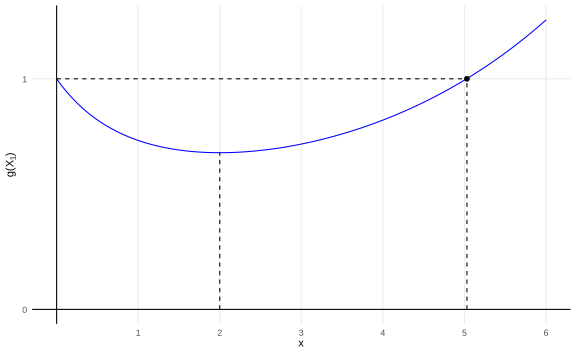
\includegraphics[width=1\linewidth]{Notas-Curso-Estadistica_files/figure-latex/unnamed-chunk-56-1} \end{center}

Entonces \((*)\) es cierto si \(X_1>c\). Se puede comprobar numéricamente que \(c\approx5.03\).

Por lo tanto, rechazamos \(H_0\) si \(X_1>5.03\).

\textbf{Criterio de Neyman-Pearson}. Encontrar un procedimiento \(\delta\) tal que

\begin{enumerate}
\def\labelenumi{\arabic{enumi})}
\item
  \(\alpha(\delta) \leq \alpha_0\) (\(\alpha_0\): nivel de significancia).
\item
  \(\beta(\delta)\) es mínimo.
\end{enumerate}

\textbf{Lema de Neyman-Pearson}. Suponga que \(\delta'\) es un procedimiento de prueba que no rechaza \(H_0\) si \(f_1(x)<kf_0(x)\) rechaza \(H_0\). Si \(f_1(x)>kf_0(x)\) y decide cualquiera de los dos si \(f_1(x)=kf_0(x)\) para \(k>0\). Si \(\delta\) es otro procedimiento de prueba tal que \(\alpha(\delta)\leq \alpha(\delta')\), entonces \(\beta(\delta)\geq \beta(\delta')\). Si \(\alpha(\delta) <\alpha(\delta')\), \(\beta(\delta)> \beta(\delta')\).

\emph{Prueba}. Tome \(a=k\) y \(b=1\) en el corolario y teoremas anteriores. Como
\[k\alpha(\delta')+\beta(\delta')\leq k\alpha(\delta')+\beta(\delta'),\]
entonces
\[\alpha(\delta)\leq \alpha(\delta')\implies \beta(\delta')\geq \beta(\delta').\]

\textbf{Consecuencia}. Si queremos encontrar una prueba \(\delta'\) que satisfaga el criterio de Neyman-Pearson, debemos encontrar \(k\) tal que \(\alpha(\delta') = \alpha_0\), y se rechace \(H_0\) si \(f_1(x)>kf_0(x) \Leftrightarrow\dfrac{f_0(x)}{f_1(x)}<k^{-1}\).

\textbf{Ejemplo}. Suponga que \(X_1,\dots,X_n\sim N(\theta,1)\) y se quiere probar \(H_0: \theta = 0\) vs \(H_1: \theta = 1\) usando una prueba según el criterio de Neyman-Pearson con \(\alpha = 0.05\).

Note que

\begin{itemize}
\tightlist
\item
  \(f_0(x) = (2\pi)^{-n/2}\exp\bigg[-\dfrac 12 \sum X_i^2\bigg]\).
\item
  \(f_1(x) = (2\pi)^{-n/2}\exp\bigg[-\dfrac 12 \sum (X_i-1)^2\bigg]\).
\end{itemize}

Entonces

\begin{align*}
\dfrac{f_1(x)}{f_0(x)}& = \exp\bigg[-\dfrac 12 \sum (X_i^2-2X_i+1-X_1^2)\bigg]\\
& = \exp\bigg[n\bar X_n - \dfrac n2\bigg] = \exp\bigg[n\left(\bar X_n - \dfrac 12\right)\bigg] 
\end{align*}

Rechazamos \(H_0\) si

\[\dfrac{f_1(x)}{f_0(x)} = \exp\bigg[n\left(\bar X_n - \dfrac 12\right)\bigg]>k \Leftrightarrow \bar X_n > \underbrace{\dfrac 12 + \dfrac{\ln k}{n}}_{k'} .\]

Entonces buscamos \(k'\) tal que
\[\mathbb P[\bar X_n>k'|\theta = 0]=0.05 \Leftrightarrow\mathbb P\bigg[\dfrac{\bar X_n}{1/\sqrt n}>\dfrac{k'}{1/\sqrt n}\bigg|\theta = 0\bigg]=0.05\]
Despejando,
\[k'\sqrt n= z_{0.95} \implies k'=\dfrac{z_{0.95}}{\sqrt n}.\]

Entonces, entre todas las pruebas en donde \(\alpha(\delta)\leq 0.05\), la que tiene el error tipo II más pequeño es la que rechaza \(H_0\) si

\[\bar X_n > \dfrac{z_{0.95}}{\sqrt n} = \dfrac{1.645}{\sqrt n}.\]

El error tipo II de esta prueba sería
\begin{align*}
\beta(\delta') = \mathbb P[\bar X_n<1.645n^{-1/2}|\theta = 1]\\
& = \mathbb P\bigg[Z < \dfrac{1.645n^{-1/2}-1}{n^{-1/2}}\bigg] = \Phi(1.645-n^{1/2})
\end{align*}

Si \(n=9\), por ejemplo, \(\beta(\delta') = \Phi(1.645-3) =0.0877.\)

\textbf{Ejemplo}. \(X_1,\dots,X_n\sim\text{Ber}(p)\) y considere las hipótesis
\[H_0: p = 0.2 \text{ vs } H_1: p = 0.4.\]

Queremos encontrar un procedimiento de prueba en donde \(\alpha(\delta) = 0.05\) y \(\beta(\delta)\) es mínimo. Sea \(y = \sum X_i\).

\[f_0(x) = 0.2^y0.8^{n-y}\]
\[f_1(x) = 0.4^y0.6^{n-y}\]

Entonces el cociente de verosimilitud es

\[\dfrac{f_1(x)}{f_0(x)}=\left(\dfrac 34\right)^n\left(\dfrac 83\right)^y\]

y se rechaza \(H_0\) si

\begin{align*}
\dfrac{f_1(x)}{f_0(x)}>k & \Leftrightarrow -n\ln \left(\dfrac 43 \right) + y \ln \left(\dfrac 83 \right)>\ln k\\ & \Leftrightarrow y>\dfrac{\ln k + n\ln(4/3)}{\ln (8/3)} = k'.
\end{align*}

Entonces basta con encontrar \(k'\) tal que

\[\mathbb P(Y>k'|p = 0.2) = 0.05,\]
pero como \(Y\) es una variable discreta (Binomial), no es posible encontrar ese \(k'\). Note que
\[\mathbb P(Y>4|p=0.2) = 0.0328\]
\[\mathbb P(Y>3|p=0.2) = 0.1209\]

Por lo tanto, se puede especificar una prueba con nivel 0.05, \(\alpha(\delta) = 0.0328\) y potencia mínima si \(Y>4\) como región de rechazo.

\hypertarget{prueba-t}{%
\section{\texorpdfstring{Prueba \(t\)}{Prueba t}}\label{prueba-t}}

Suponga que \(X_1,\dots, X_n \sim N(\mu,\sigma^2)\), con \((\mu,\sigma^2)\) desconocidos, y considere las siguientes hipótesis:

\[H_0: \mu\leq\mu_0 \text{ vs } H_1:\mu>\mu_0.\]

Recuerde que si \(U = \dfrac{\bar X_n -\mu_0}{\sigma' /\sqrt n}\), entonces la prueba rechaza \(H_0\) si \(U\geq c\). Si \(\mu=\mu_0\) entonces \(U \sim t_{n-1}\).

Si \(H_0: \mu\geq\mu_0\) vs \(H_1: \mu<\mu_0\), entonces se rechaza \(H_0\) si \(U\leq c\).

\textbf{Definición}. Considere las hipótesis \(H_0:\theta \in \Omega_0\) vs \(H_1: \theta\in \Omega_1\). Decimos que una prueba de hipótesis \(\delta\) es \textbf{insesgada} si \(\forall \theta\in\Omega_0\) y \(\forall \theta\in \Omega_1\):
\[\pi(\theta|\delta) \leq \pi(\theta'|\delta).\]

\hypertarget{propiedades-de-las-pruebas-t}{%
\subsection{\texorpdfstring{Propiedades de las pruebas \(t\)}{Propiedades de las pruebas t}}\label{propiedades-de-las-pruebas-t}}

\textbf{Teorema}. Sea \(X_1,\dots,X_n\sim N(\mu,\sigma^2)\). Sea \(U\) definido anteriormente, \(c=t_{n-1,1-\alpha_0}\). Sea \(\delta\) la prueba que rechaza \(H_0\) si \(U\geq c\). Entonces

\begin{enumerate}
\def\labelenumi{\roman{enumi})}
\item
  \(\pi(\mu,\sigma^2|\delta) = \alpha_0\) si \(\mu=\mu_0\).
\item
  \(\pi(\mu,\sigma^2|\delta) < \alpha_0\) si \(\mu>\mu_0\).
\item
  \(\pi(\mu,\sigma^2|\delta) >\alpha_0\) si \(\mu>\mu_0\).
\item
  \(\pi(\mu,\sigma^2|\delta) \to 0\) si \(\mu\to-\infty\).
\item
  \(\pi(\mu,\sigma^2|\delta) \to 1\) si \(\mu\to+\infty\).
\end{enumerate}

Entonces, la prueba tiene tamaño \(\alpha_0\) y es insesgada.

\emph{Prueba}. Ver en el libro.

En el caso en donde \(H_0:\mu\geq \mu_0\) las desigualdades se intercambian y la prueba también tiene tamaño \(\alpha_0\) y es insesgada.

\textbf{Teorema}. Bajo cualquiera de los dos casos anteriores, sea \(U\) el valor observado de \(U\). Entonces, el valor-\emph{p} de la prueba \(\delta\) que rechaza \(H_0: \mu\leq\mu_0\) es \(1-T_{n-1}(u)\) donde \(T_{n-1}\) es c.d.f de \(t_{n-1}\) y si se rechaza \(H_0 \mu\geq \mu_0\), el valor-\emph{p} es \(T_{n-1}(u)\).

\emph{Prueba}. El caso \(H_0:\mu\leq\mu_0\) es análogo al cálculo del valor-\emph{p} que se hizo en el capítulo anterior. El caso \(H_0: \mu\geq \mu_0\) se rechaza si \[U\leq T_{n-1}^{-1}(\alpha_0) \Leftrightarrow T_{n-1}(u)\leq \alpha_0.\]
Es decir, el nivel más pequeño de significancia observada es \(T_{n-1}(u)\)

Considere el caso \(H_0: \mu\geq \mu_0\) vs \(H_1: \mu>\mu_0\).

\begin{itemize}
\item
  Región de rechazo: \(U\geq c\) con \(U= \dfrac{\bar X_n -\mu_0}{\sigma' /\sqrt n}\).
\item
  \emph{Ejercicio}: es una prueba insesgada con nivel \(\alpha_0\) si \(c = t_{n-1,1-\alpha_0}\).
\item
  Valor-\emph{p}: si observamos \(U=u\), se rechaza \(H_0\) si \(u\geq t_{n-1,1-\alpha_0}\),
\end{itemize}

\[T_{n-1}(u) \geq T_{n-1}(t_{n-1,1-\alpha_0}) = 1-\alpha_0 \implies 1-T_{n-1(u)} = T_{n-1}(u).\]

\begin{itemize}
\tightlist
\item
  Función de potencia:
\end{itemize}

\begin{align*}
\mathbb P[\text{Rechazo}|\mu] & = \mathbb P\bigg[ \dfrac{\bar X_n -\mu_0}{\sigma' /\sqrt n}\geq t_{n-1,1-\alpha_0}\bigg| \mu \bigg]\\
&= = \mathbb P\bigg[ \dfrac{\bar X_n +\mu-\mu-\mu_0}{\sigma' /\sqrt n}\geq t_{n-1,1-\alpha_0}\bigg| \mu \bigg]\\
& = \mathbb P\bigg[ \underbrace{\dfrac{\bar X_n -\mu}{\sigma' /\sqrt n}}_{\Delta}+ \dfrac{\mu-\mu_0}{\sigma' /\sqrt n}\geq t_{n-1,1-\alpha_0}\bigg| \mu \bigg]\\
\end{align*}

Observe que

\[\Delta = \dfrac{\bar X_n -\mu}{\sigma' /\sqrt n}\cdot\dfrac\sigma\sigma = \dfrac{\dfrac{\sqrt n(\bar X_n-\mu)}{\sigma} \sim N(0,1)}{\dfrac{\sigma'}\sigma = \sqrt{\dfrac{\chi^2}{n-1}}} \sim t_{n-1}.\]

De igual forma, vea que

\[ U = \dfrac{\dfrac{\sqrt n(\bar X_n-\mu_0)}{\sigma}}{\dfrac{\sigma'}{\sigma}} =  \dfrac{\dfrac{\sqrt n}{\sigma}(\bar X_n-\mu) +\overbrace{\dfrac{\sqrt n}{\sigma}(\mu-\mu_0)}^{\psi}  \sim N(\psi,1)}{\dfrac{\sigma'}{\sigma}}.\]

\textbf{Definición}. Si \(Y\), \(W\) son independientes con \(W\sim N(\psi,1)\) y \(Y\sim \chi^2_m\), entonces \(X\) se distribuye como una \textbf{\(t\)-Student no centrada} con parámetro \(\psi\) si
\[X = \dfrac W{\sqrt{\dfrac{Y}{m}}}.\]

Si \(T_m(t|\psi)\) es c.d.f de \(X\), entonces
\[\pi(\mu|\delta)= T_{n-1}(t_{n-1,1-\alpha_0}).\]

En el caso que la prueba sea \(H_0: \mu\leq \mu_0\) vs \(H_1: \mu<\mu_0\).

\[\pi(\mu|\delta)= \mathbb P[U\leq t_{n-1,1-\alpha_0}] = T_{n-1}(t_{n-1,\alpha_0}).\]

\textbf{Conclusión}: a partir del error tipo II se puede determinar un tamaño de muestra dado, siempre y cuando existan restricciones sobre \(\mu\) y \(\sigma^2\).

\hypertarget{prueba-t-pareada}{%
\subsection{\texorpdfstring{Prueba \(t\) pareada}{Prueba t pareada}}\label{prueba-t-pareada}}

\textbf{Ejemplo}. Considere una muestra de \(n\) pacientes que fuman \(X\) cantidad al día. Sean \(t_1\) el momento de la observación y \(t_2\) el tratamiento. El consumo de cigarrillos en el individuo \#\emph{i} es

\[D_i = X_i^{t_2}-X_i^{t_1},\quad i = 1,\dots,n.\]

Otro ejemplo es tomar \(Y_i^{t_1,t_2}\) el log-daño en los muñecos de prueba, donde \(t_1\) corresponde al conductor y \(t_2\) al acompañante, entonces

\(X_i = Y_i^{t_1}-Y_i^{t_2} = \ln\left(\dfrac{\text{da}\tilde{\text n}\text{o}^{t_1}}{\text{da}\tilde{\text n}\text{o}^{t_2}}\right) \implies \text{da}\tilde{\text n}\text{o}^{t_2}\cdot e^{X_i} = \text{da}\tilde{\text n}\text{o}^{t_1}\)

Evaluemos la prueba \(H_0:\mu\leq 0\) vs \(H_1:\mu>0\) al 1\%. Si \(X_1,\dots, X_n \sim N(\mu,\sigma^2)\) ambos parámetros desconocidos, y \(n=164\), \(\bar X_n = 0.2199\), \(\sigma'=0.5342\), rechazamos \(H_0\) si

\[U = \dfrac{0.2199-0}{\dfrac{0.5342}{\sqrt {164}}} = 5.271 >t_{163,1-0.01} = 2.35.\]

El valor-\emph{p} de la prueba es
\[1-\mathbb P[t_{163}<5.271] = 1\times10^{-6}<1\%.\]
Entonces rechazo \(H_0\) con nivel de significancia de \(1%
\).

Suponga que la diferencia media entre conductor y pasajero es \(\dfrac\sigma 4\). ¿Cuál es el error tipo II?

\[\mu =\dfrac\sigma 4\implies \psi = \dfrac{\mu-\mu_0}{\sigma/\sqrt n} = \dfrac{\sigma/4-0}{\sigma/\sqrt{164}} = \dfrac{\sqrt{164}}{3} = 3.2.\]

El error tipo II es \(T_{163}(2.35|\psi =3.2) = 1-0.802 = 0.198\).

\hypertarget{pruebas-t-de-dos-colas}{%
\subsection{\texorpdfstring{Pruebas \(t\) de dos colas}{Pruebas t de dos colas}}\label{pruebas-t-de-dos-colas}}

\begin{itemize}
\item
  Región de rechazo: \(|U|\geq t_{n-1,1-\frac{\alpha_0}2}\).
\item
  Función de potencia:
\end{itemize}

\[\pi(\mu|\delta) = \mathbb P[U\geq t_{n-1,1-\frac{\alpha_0}2}|\mu]+\mathbb P[U\leq t_{n-1,1-\frac{\alpha_0}2}|\mu] = T_{n-1}(-c|\psi) + 1-T_{n-1}(c|\psi). \]

\begin{itemize}
\tightlist
\item
  Valor-\emph{p}: si observamos \(U=u\), rechazamos \(H_0\) si
\end{itemize}

\[|u|\geq t_{n-1,1-\frac{\alpha_0}2} \Leftrightarrow T_{n-1}(|U|)\geq 1-\dfrac{\alpha_0}2 \Leftrightarrow \alpha_0\geq \underbrace{2[1-T_{n-1}(|u|)]}_{\text{valor-}p}.\]

\textbf{Propiedad}. La prueba-\(t\) unilateral es un LRT.

Sea \(f_n(x|\mu)\) la función de verosimilitud de una muestra de distribuciones normales y considere
\[\Lambda(x) = \dfrac{\sup_{\mu\leq\mu_0}f_n(x|\mu)}{\sup_{\mu}f_n(x|\mu)}. \]

El MLE en \(\Omega\) es \((\bar X_n,\hat\sigma^2)\), entonces

\[\sup_{\mu}f_n(x|\mu) = \dfrac1{(2\pi\hat\sigma^2)^{n/2}}e^{-n/2}.\]

El MLE en \(\Omega_0\), si \(\bar X_n<\mu_0\) es \(\bar X_n\), por lo que \(\Lambda(x) =1\).

Si \(\bar X_n>\mu_0\), se puede probar que \(f_n(x|\mu)\) se maximiza si \(\mu\) está lo más cerca posible de \(\bar X_n\), que, en el subconjunto \(\Omega_0\) sería \(\mu_0\). Entonces \(\mu = \mu_0\), \(\hat\sigma_0 = \dfrac 1n \sum_{i=1}^n(X_i-\mu_0)^2\) y
\[\sup_{\mu}f_n(x|\mu) = \dfrac1{(2\pi\hat\sigma_0^2)^{n/2}}e^{-n/2}.\]

Por lo tanto
\(\Lambda(x) = \begin{cases}\left(\dfrac{\hat \sigma^2}{\hat\sigma_0^2}\right)^{n/2}& \text{si }\bar X_n>\mu_0\\ 1 & \text{si no}\end{cases}\)

\emph{Ejercicio}: si \(u\) es el valor observado del estadístico \(U\), verifique que \(\Lambda(x)\) es monótono decreciente con respecto a \(u\).

Por lo tanto, para \(k<1\) existe \(c\) tal que
\[\Lambda(x) \leq k \Leftrightarrow u\geq c.\]

\emph{Ejercicio}: encuentre \(c\).

Se concluye que LRT es una prueba \(t\).

\hypertarget{prueba-de-comparaciuxf3n-de-medias-en-2-poblaciones}{%
\chapter{Prueba de comparación de medias en 2 poblaciones}\label{prueba-de-comparaciuxf3n-de-medias-en-2-poblaciones}}

\hypertarget{comparaciuxf3n-de-medias-normales}{%
\section{Comparación de medias normales}\label{comparaciuxf3n-de-medias-normales}}

Asuma que \(X_1,\dots, X_n\overset{i.i.d}{\sim} N(\mu_1,\sigma^2)\) y \(Y_1,\dots, Y_n\overset{i.i.d}{\sim} N(\mu_2,\sigma^2)\). Los parámetros desconocidos son \(\mu_1,\mu_2,\sigma^2\). Asuma que \((X_i,Y_i)\) son independientes y la varianza es la misma (homocedasticidad).

\textbf{Hipótesis}: \(H_0: \mu_1\leq\mu_2\) vs \(H_1: \mu_1>\mu_2\).

\textbf{Notación}: \(\bar X_m,\bar Y_n\), \(S_X^2 = \sum_{i=1}^m(X_i-\bar X_m)^2\), \(S_Y^2 = \sum_{i=1}^m(Y_i-\bar Y_n)^2\).

\textbf{Teorema}. Considere
\[U = \dfrac{(m+n-2)^{1/2}(\bar X_m-\bar Y_n)}{\left(\dfrac 1m+\dfrac 1n\right)^{1/2}(S_X^2+S_Y^2)^{1/2}}.\]
Si \(\mu_1=\mu_2 \implies U\sim t_{m+n-2}.\)

\emph{Prueba}. Vea que, bajo el supuesto que \(\mu_1=\mu_2\), \(\bar X_n-\bar Y_n\) se distribuye como una normal con parámetros:

\begin{itemize}
\item
  \(\mathbb E[X_n-\bar Y_n] = \mu_1-\mu_2 =0\).
\item
  \(\text{Var}(\bar X_m-\bar Y_n) =\text{Var}(\bar X_m) + \text{Var}(\bar Y_n) = \dfrac{\sigma^2}m + \dfrac{\sigma^2}n =\left(\dfrac 1m+\dfrac 1n\right)\sigma^2\).
\end{itemize}

Entonces
\[Z = \dfrac{\bar X_m-\bar Y_n}{\sigma\left(\dfrac 1m+\dfrac 1n\right)^{1/2}}\underset{\mu_1 =\mu_2}{\sim} N(0,1).\]
Así mismo, se sabe que \(\dfrac{S_X^2}{\sigma^2}\sim \chi^2_{m-1}\) y \(\dfrac{S_Y^2}{\sigma^2}\sim \chi^2_{n-1}\).

\textbf{Nota}: no depende de \(H_0\).

Como \((X,Y)\) son independientes, \(\dfrac{S_X^2}{\sigma^2}\) y \(\dfrac{S_Y^2}{\sigma^2}\) son independientes. Así,

\[W = \dfrac{S_X^2+S_Y^2}{\sigma^2} \sim \chi^2_{m+n-2}.\]

Entonces

\[U = \dfrac{Z}{\sqrt{\dfrac W{m+n-2}}}=\dfrac{\dfrac{\bar X_m-\bar Y_n}{\sigma\left(\dfrac 1m+\dfrac 1n\right)^{1/2}}}{\sqrt{\dfrac 1{m+n-2}\left(\dfrac{S_X^2+S_Y^2}{\sigma^2}\right)}}\sim t_{m+n-1}.\]

\hypertarget{prueba-t-de-dos-muestras}{%
\section{\texorpdfstring{Prueba \(t\) de dos muestras}{Prueba t de dos muestras}}\label{prueba-t-de-dos-muestras}}

Dada una región de rechazo \(U\geq c\),
\begin{align*}
\sup_{\mu_1\leq \mu_2}\mathbb P[U\geq c|\mu_1,\mu_2,\sigma^2]\leq \alpha_0 & \implies \mathbb P[U\geq c|\mu_1=\mu_2,\sigma^2] = 1-T_{n+m-2}(c) \leq \alpha_0 \\
& \implies c = T_{n+m-2}^{-1}(1-\alpha_0)
\end{align*}

Rechazo \(H_0\) si \(U> T_{n+m-2}^{-1}(1-\alpha_0): \delta\).

\textbf{Teorema}. La función de potencia \(\pi(\mu_1,\mu_2,\sigma^2|\delta)\) tiene las siguientes propiedades:

\begin{enumerate}
\def\labelenumi{\roman{enumi}.}
\item
  \(\pi(\mu_1,\mu_2,\sigma^2|\delta) = \alpha_0\) si \(\mu_1 = \mu_2\).
\item
  \(\pi(\mu_1,\mu_2,\sigma^2|\delta) < \alpha_0\) si \(\mu_1 < \mu_2\).
\item
  \(\pi(\mu_1,\mu_2,\sigma^2|\delta) > \alpha_0\) si \(\mu_1 > \mu_2\).
\end{enumerate}

\textbf{Conclusión}. \(\delta\) es una prueba insesgada con tamaño \(\alpha_0\).

\begin{enumerate}
\def\labelenumi{\roman{enumi}.}
\setcounter{enumi}{3}
\tightlist
\item
  Los límites cuando \(\mu_1-\mu_2\to -\infty (+\infty)\) son los mismos del caso de una muestra.
\end{enumerate}

Observe que para el caso II: \(H_0: \mu_1\geq\mu_2\) vs \(H_1: \mu_1<\mu_2\).

\[\delta: \text{Rechazo } H_0 \text{ si } U<T^{-1}_{n+m-2}(\alpha_0) = -T_{n+m-2}^{-1}(1-\alpha_0).\]

Los \emph{p}-valores son:

\begin{itemize}
\item
  Caso I: \(1-T_{n+m-2}(u)\) si observamos \(U = u\).
\item
  Caso II: \(T_{n+m-2}(u)\).
\end{itemize}

\textbf{Ejemplo}. Considere la log-precipitación de 26 observaciones de nubes con químicos, \(X_1,\dots,X_{26}\) y 26 sin químicos \(Y_1,\dots,Y_{26}\).

\emph{Supuestos}: \(X_i\sim N(\mu_1,\sigma^2)\), \(Y_j\sim N(\mu_2,\sigma^2)\).

\emph{Hipótesis}: \(H_0: \mu_1\leq\mu_2\) vs \(H_1: \mu_1>\mu_2\).

Con los siguientes datos: \(\bar X_m = 5.13\), \(\bar Y_n = 3.99\), \(S_X^2 = 63.96\), \(S_Y^2=67.39\), se tiene que

\[U = \dfrac{50^{1/2}(5.13-3.99)}{\left(\dfrac{1}{26}+\dfrac{1}{26}\right)^{1/2}(63.96+67.39)^{1/2}} = 2.544.\]

A un nivel de confianza del 99\% ,

\[ T_{n+m-2}(1-\alpha_0) = T_{50}^{-1}(99\%) = 2.403 \implies U > T^{-1}_{50}(99\%)\]

y el valor-\emph{p}: \(1-T_{50}(2.544) = 0.007\).

\emph{Interpretación}: rechazamos al nivel 1\% de significancia la hipótesis de que las nubes irradiadas tienen una log-precipitación media menor a la de las nubes no irradiadas.

\hypertarget{prueba-de-2-colas}{%
\subsection{Prueba de 2 colas}\label{prueba-de-2-colas}}

\textbf{Hipótesis}. \(H_0: \mu_1=\mu_2\) vs \(H_1: \mu_1\ne\mu_2\) (Prueba ANOVA).

\begin{itemize}
\item
  Prueba. \(\delta:\) Rechazo \(H_0\) si \(|U|\geq T^{-1}_{m+n-2}\left(1-\dfrac{\alpha_0}2\right)\).
\item
  Valor-\emph{p}: \(2-T_{m+n-2}(|u|)\) donde \(U=u\).
\end{itemize}

\textbf{Ejemplo}. Menas de cobre. Sean \(X_1,\dots,X_8\) la cantidad de cobre (g) en 8 menas en la localización 1, y \(X_1,\dots,X_{10}\) en 10 menas en la localización 2. Los datos son \(\bar X_8 = 2.6,\bar Y_{10} = 2.3, S_X^2 = 0.32\) y \(S_Y^2=0.22\) ¿Las dos localizaciones generan el mismo nivel de cobre?

\(H_0: \mu_1=\mu_2\), \(X_i\sim N(\mu_1,\sigma^2)\), \(Y_j\sim N(\mu_2,\sigma^2)\).

Se tiene que \(U = 3.442\).Si \(\alpha_0 = 1\%\), \(T^{-1}_{16}\left(1-\dfrac{0.01}2\right) = T_{16}^{-1}(0.995) = 2.921\).

Rechazamos \(H_0\) pero el valor-\emph{p} es \(2[1-T_{16}(|3.442|)] = 0.003\).

\emph{Interpretación}: rechazamos al 1\% de significancia la hipótesis de una diferencia no significativa entre las cantidades medias de cobre en cada localización.

\textbf{Ejercicio}. La prueba \(t\) de 2 muestras es un LRT.

\hypertarget{prueba-f}{%
\section{\texorpdfstring{Prueba \(F\)}{Prueba F}}\label{prueba-f}}

\textbf{Definición} Si \(Y\) y \(W\) son variables aleatorias independientes, \(Y\sim \chi^2_m\) y \(W\sim \chi ^2_n\), \(m,n\in \mathbb Z^+\). Defina
\[X = \dfrac{Y/m}{W/n}\sim F_{m,n}\]
\(X\) tiene una distribución \(F\) con \(m\) y \(n\) grados de libertad.

\textbf{Propiedades}:

\begin{enumerate}
\def\labelenumi{\arabic{enumi}.}
\item
  Si \(X\sim F_{m,n} \implies 1/X\sim F_{n,m}\).
\item
  Si \(Y\sim t_n \implies Y^2\sim F_{1,n}\).
\end{enumerate}

Sean \(X_1,\dots, X_n\overset{i.i.d}{\sim} N(\mu_1,\sigma_1^2)\) y \(Y_1,\dots, Y_n\overset{i.i.d}{\sim} N(\mu_2,\sigma_2^2)\).

Considere el esquema
\begin{align*}
U\sim t_{n-1}\text{  }& \quad \quad U^2\sim F_{1,n-1}\\
H_0: \mu=\mu_0\text{  } & \Leftrightarrow \text{  }  H_0: \mu=\mu_0 \\
|U|\geq |c|\text{  } & \quad \quad  U^2\geq c^* 
\end{align*}

Bajo el esquema anterior y si \((X,Y)\) son independientes, considere:

\[H_0: \sigma_1^2\leq \sigma_2^2 \text { vs } H_1: \sigma_1^2> \sigma_2^2 \]
y tome \(\alpha_0 \in (0,1)\).

La lógica de esta prueba es, como \(\dfrac{S_X^2}{\sigma_1^2} \sim \chi^2_{m-1}\) y \(\dfrac{S_X^2}{\sigma_1^2} \sim \chi^2_{n-1}\), calculamos

\(V^* = \dfrac{\dfrac{S_X^2/\sigma_1^2}{m-1}}{\dfrac{S_Y^2/\sigma_1^2}{n-1}}\sim F_{m-1,n-1}\).
Bajo el supuesto de homocedasticidad,

\(V = \dfrac{\dfrac{S_X^2}{m-1}}{\dfrac{S_Y^2}{n-1}}\sim F_{m-1,n-1}\).

\(\delta:\) Rechazo \(H_0\) si \(V\geq c\).

\textbf{Teorema}. La distribución de \(V^*\sim F_{m-1,n-1}\) y si \(\sigma_1=\sigma_2\), \(V \sim F_{m-1,n-1}\).

Usando el \(\delta\) anterior

\[\sup_{\sigma_1^2\leq\sigma^2_2}\mathbb P[V\geq c|\mu_1\mu_2,\sigma^2_1,\sigma_2^2]\leq \alpha_0,\]
resuelve
\[\mathbb P[V\geq c|\mu_1,\mu_2,\sigma_1^2,\sigma_2^2] = \alpha_0 \implies c = F^{-1}_{m-1,n-1}(1-\alpha_0) =: G^{-1}_{m-1,n-1}(1-\alpha_0).\]

\textbf{Teorema}. si \(\delta\) se define según lo anterior,

\begin{enumerate}
\def\labelenumi{\roman{enumi}.}
\item
  \begin{align*}
  \pi(\mu_1,\mu_2,\sigma_1^2,\sigma_2^2|\delta) & = \mathbb P[V\geq G^{-1}_{m-1,n-1}(1-\alpha_0)]\\
  & = \mathbb P\bigg[V^* \geq \dfrac{\sigma_2^2}{\sigma_1^2}c\bigg]\\
  & = 1-G_{m-1,n-1}\left(\dfrac{\sigma_2^2}{\sigma_1^2}c\right)
  \end{align*}
\item
  \(\pi(\mu_1,\mu_2,\sigma_1^2,\sigma_2^2,|\delta) = \alpha_0\) si \(\sigma_1^2 = \sigma_2^2\).
\item
  \(\pi(\mu_1,\mu_2,\sigma_1^2,\sigma_2^2|\delta) < \alpha_0\) si \(\sigma_1^2 < \sigma_2^2\).
\item
  \(\pi(\mu_1,\mu_2,\sigma_1^2,\sigma_2^2|\delta) > \alpha_0\) si \(\sigma_1^2 > \sigma_2^2\).
\item
  \(\dfrac{\sigma_1^2 }{\sigma_2^2 }\to 0 \implies \pi \to 0\).
\item
  \(\dfrac{\sigma_1^2 }{\sigma_2^2 }\to \infty \implies \pi \to 1\).
\end{enumerate}

Por (i)-(iv) \(\delta\) es insesgada con tamaño \(\alpha_0\).

El valor-\emph{p} es \(1-G_{m-1,n-1}(v)\), \(V=v\).

\textbf{Ejemplo}. \(X_1,\dots,X_{6}\sim N(\mu_1,\sigma_1^2)\), \(S_X ^2 =30\), \(Y_1,\dots,Y_{21}\sim N(\mu_2,\sigma_2^2)\), \(S_Y^2=30\).

La hipótesis nula es \(H_0: \sigma_1^2\leq \sigma_2^2\).

Se calcula \(V = \dfrac{30/5}{40/20} = 3\) y \(F^{-1}_{5,20}(1-0.05) = 2.71.\)

El valor-\emph{p} corresponde a \(1-G_{5,20}(3) = 0.035.\)

Si \(\alpha_0 = 1\%\), no rechazo. Si \(\alpha_0 = 5\%\) rechazo.

\hypertarget{prueba-de-2-colas-prueba-de-homocedasticidad}{%
\subsection{Prueba de 2 colas (prueba de homocedasticidad)}\label{prueba-de-2-colas-prueba-de-homocedasticidad}}

Bajo las hipótesis \(H_0: \sigma^2_1=\sigma^2_2\) vs \(H_1: \sigma^2_1\ne\sigma^2_2\), se rechaza si \(V\geq c_2\) o \(V\leq c_1\) con \(c_1,c_2\) tales que
\[\mathbb P[V\leq c_1] = \dfrac{\alpha_0}{2} \text{ y } \mathbb P[V\geq c_2] = \dfrac{\alpha_0}{2} \implies c_1 = G_{m-1,n-1}^{-1}\left(\dfrac{\alpha_0}{2}\right) c_1 = G_{m-1,n-1}^{-1}\left(\dfrac{\alpha_0}{2}\right)\]

\textbf{Ejemplo}. Mismo ejemplo de las nubes. Queremos probar \(H_0:\sigma_1^2 = \sigma_2^2\). Calculamos

\[V = \dfrac{\dfrac{63.96}{25}}{\dfrac{67.39}{25}} = 0.9491\]

Se tiene que \(c_1 = G^{-1}_{25,25}(0.0025) = 0.4484\) y \(c_2 = G^{-1}_{25,25}(0.975) = 2.23\).

Si observamos \(V=v\), podemos rechazar si\\
\[
v\leq G^{-1}_{m-1,n-1}\left(\dfrac{\alpha_0}2\right) \implies 2G_{m-1,n-1}(v)\leq \alpha_0
\]

o tambien si

\[v\geq G^{-1}_{m-1,n-1}\left(1-\dfrac{\alpha_0}2 \right) \implies G_{m-1,n-1}(v) \geq 1-\dfrac{\alpha_0}2 \implies \alpha_0\geq 2G_{m-1,n-1}(v) \]

Por lo tanto, el \emph{p}-valor es
\[\text{valor-}p = 2\min[1-G_{m-1,n-1}(v), G_{m-1,n-1}(v)]\]

\textbf{Ejercicio}. Verifique que en este caso da 0.9.

Al ser mayor al 5\%, no rechaza la hipótesis de homocedasticidad.

\textbf{Propiedad}. La prueba \(F\) es un LRT.

\hypertarget{pruebas-de-hipuxf3tesis-bayesianas}{%
\chapter{Pruebas de hipótesis bayesianas}\label{pruebas-de-hipuxf3tesis-bayesianas}}

\hypertarget{pruebas-de-hipuxf3tesis-bayesianas-1}{%
\section{Pruebas de hipótesis bayesianas}\label{pruebas-de-hipuxf3tesis-bayesianas-1}}

Suponga que \(\Omega = \{\theta_0,\theta_1\}\). Si \(\theta = \theta_i\) \((i = 0,1)\), \(X_1,\dots, X_n\sim f_i(x)\). Considere las hipótesis
\[H_0: \theta = \theta_0 \text{ vs } H_1: \theta =\theta_1.\]
Hay dos decisiones, \(d_0:\) no rechazo \(H_0\) y \(d_1:\) rechazo \(H_0\).

Asuma que si selecciono \(d_1\) cuando \(H_0\) es cierto, la pérdida es \(w_0\). Por el contrario, si selecciono \(d_1\) cuando \(H_0\) es cierto, la pérdida es \(w_1\).

\begin{longtable}[]{@{}lll@{}}
\toprule
& \(d_0\) & \(d_1\)\tabularnewline
\midrule
\endhead
\(\theta_0\) & 0 & \(w_0\)\tabularnewline
\(\theta_1\) & \(w_1\) & 0\tabularnewline
\bottomrule
\end{longtable}

Sean \(\pi_0 = \mathbb P[H_0 \text{ es cierta}] = \mathbb P[H_0]\) y \(\pi_1 = \mathbb P[H_1 \text{ es cierta}] = 1 -\mathbb P[H_0]\).

Considere \(\delta\) el procedimiento de prueba. El valor esperado de la pérdida corresponde a

\[ r(\delta)  = \mathbb E[\text{Pérdida}|H_0] \mathbb P[H_0] + \mathbb E[\text{Pérdida}|H_1]\mathbb P[H_1].\]

Dado \(H_0\),

\begin{align*}
\mathbb E[\text{Pérdida}|H_0] & = w_0\cdot \mathbb P[\text{Seleccione } d_1|\theta_0] + 0\cdot \mathbb P[\text{Seleccione } d_0|\theta_0]\\
& = w_0 \cdot \text{Error I} = w_0\alpha(\delta).
\end{align*}
Por el otro lado,

\begin{align*}
\mathbb E[\text{Pérdida}|H_1] & = 0\cdot \mathbb P[\text{Seleccione} d_1|\theta_0] + w_1\cdot \mathbb P[\text{Seleccione} d_0|\theta_0]\\
& = w_1 \cdot \text{Error II} = w_1\beta(\delta).
\end{align*}

Entonces \(r(\delta) = w_0\alpha(\delta) + w_1\beta(\delta)\).

El procedimiento \(\delta\) que minimiza \(r(\delta)\) se llama procedimiento de prueba bayesiana. Por el teorema de Neyman-Pearson y tomando \(a=\pi_0w_0\) y \(b=\pi_1w_1\), el \(\delta\) que soluciona el problema es:

\[\delta: \text{Rechazo }H_0 \text{ si } \pi_0w_0f_0(x) < \pi_1w_1f_1(x). \]

o si \(\pi_0w_0f_0(x) = \pi_1w_1f_1(x)\), \(\dfrac{f_1(x)}{f_0(x)} > \dfrac ab = k\).

\textbf{Nota}. La decisión \(\delta\) es invariante a multiplicacione por escalar en el costo.

\textbf{Ejemplo}.

\begin{enumerate}
\def\labelenumi{\alph{enumi}.}
\tightlist
\item
  Calculemos
\end{enumerate}

\[\pi(\theta_0|x) = \dfrac{\pi_0f_0(x)}{\pi_0f_0(x)+\pi_1f_1(x)}\]
\[\pi(\theta_1|x) = \dfrac{\pi_1f_1(x)}{\pi_0f_0(x)+\pi_1f_1(x)}\]

\begin{enumerate}
\def\labelenumi{\alph{enumi}.}
\setcounter{enumi}{1}
\tightlist
\item
  Esperanza de la pérdida
\end{enumerate}

\[\mathbb E[\text{Pérdida}|x] = \mathbb E[\text{Pérdida}|\theta_0,x] + \mathbb E[\text{Pérdida}|\theta_1,x].\]

Si \(\delta = d_0\),

\[\mathbb E_\delta[\text{Pérdida}|X] = w_1\pi(\theta_1|x) =  \dfrac{w_1\pi_1f_1(x)}{\pi_0f_0(x)+\pi_1f_1(x)}. \]

Si \(\delta = d_1\),

\[\mathbb E_\delta[\text{Pérdida}|X] = \dfrac{w_0\pi_0f_0(x)}{\pi_0f_0(x)+\pi_1f_1(x)}. \]

Minimizar \(\mathbb E[\text{Pérdida}|x]\) con respecto a \(\delta\) es equivalente a rechazar \(H_0\) bajo el criterio anterior.

\textbf{Conclusión}: es equivalente construir la decisión en cualquiera de los dos criterios (previa o probabilidad posterior).

\begin{enumerate}
\def\labelenumi{\alph{enumi}.}
\setcounter{enumi}{2}
\tightlist
\item
  Rechazo \(H_0\) si \(\mathbb P[H_0 \text{ es cierto}|X] \leq \dfrac{w_1}{w_0+w_1}.\)
\end{enumerate}

Rechazamos \(H_0\) si
\[\dfrac{w_0\pi_0f_0(x)}{\pi_0f_0(x)+\pi_1f_1(x)}\leq \dfrac{w_1\pi_1f_1(x)}{\pi_0f_0(x)+\pi_1f_1(x)}.\]

Entonces

\[w_0\mathbb P[H_0|x] \leq w_1\mathbb P[H_1|x] = w_1[1-\mathbb P[H_0|x]] \implies\mathbb P[H_0|x]\leq \dfrac{w_1}{w_0+w_1}. \]

\emph{Caso general}: \(H_0: \theta \in \Omega_0\) vs \(H_1: \theta \in \Omega_1\).

\hypertarget{hipuxf3tesis-de-una-cola}{%
\section{Hipótesis de una cola}\label{hipuxf3tesis-de-una-cola}}

Asuma la misma función de pérdida \(L(\theta,d_i)\):

\begin{longtable}[]{@{}lll@{}}
\toprule
& \(d_0\) & \(d_1\)\tabularnewline
\midrule
\endhead
\(H_0\) & 0 & \(w_0\)\tabularnewline
\(H_1\) & \(w_1\) & 0\tabularnewline
\bottomrule
\end{longtable}

y considere la hipótesis \(H_0: \theta \leq \theta_0\) vs \(H_1: \theta > \theta_0\).

\textbf{Teorema}. Suponga que \(f_n(x|\theta)\) tiene un cociente de verosimilitud monótono con respecto al estadístico \(T=r(x)\). Es decir,
\(R(x) = \dfrac{f_n(x|\theta_1)}{f_n(x|\theta_0)} = g(r(x))\)
con \(g(r(x))\) monótono con respecto a \(r(x)\).

Asuma la función de pérdida anterior. Entonces el procedimiento bayesiano de prueba rechaza \(H_0\) cuando \(T\geq c\).

\textbf{Definición}. Si \(f_n(x|\theta)\) es una verosimilitud y \(T=r(x)\) un estadístico, decimos que \(f_n(x|\theta)\) tiene un MLR con respecto a \(T\) si para \(\theta_1,\theta_2 \in \Omega\) tales que \(\theta_1 <\theta_2\), \(\dfrac{f_n(x|\theta_2)}{f_n(x|\theta_1)}\) depende de \(x\) a través de \(r(x)\) y es una función monótona de \(r(x)\).

\textbf{Ejemplo}. \(X_1,\dots, X_n \sim N(\mu,\sigma^2)\), \(\sigma^2\) conocido.
Si \(\mu_1<\mu_2\):

\begin{align*}
\dfrac{f_n(x|\mu_2)}{f_n(x|\mu_1)} & = \dfrac{(2\pi\sigma^2)^{-n/2}\exp\bigg[-\dfrac 1{2\sigma^2}\sum (X_i-\mu_2)^2\bigg]}{(2\pi\sigma^2)^{-n/2}\exp\bigg[-\dfrac 1{2\sigma^2}\sum (X_i-\mu_1)^2\bigg]}\\
& = \exp\bigg[\dfrac{n(\mu_2-\mu_1)}{\sigma^2}\bar X_n -\dfrac 12 (\mu_2+\mu_1))\bigg] = g(T)
\end{align*}

Entonces \(g(T)\) es monótono creciente con respecto a \(T=\bar X_n\) y por lo tanto tiene un MLE con respecto a \(\bar X_n\).

\emph{Prueba}. Recuerde que

\[\pi(\theta|x) = \dfrac{f_n(x|\theta)\pi(\theta)}{\int f_n(x|\psi)\pi(\psi)d\psi}\]

\begin{align*}
\mathcal L(x) = \dfrac{\mathbb E[\text{Pérdida}|x,d_0]}{\mathbb E[\text{Pérdida}|x,d_1]} & = \dfrac{\dfrac 1{\text{cte}} \displaystyle\int_{\theta_0}^\infty w_1f_n(x|\theta)\pi(\theta)d\theta}{\dfrac 1{\text{cte}} \displaystyle\int_{-\infty}^{\theta_0} w_0f_n(x|\theta)\pi(\theta)d\theta} \\ & = \dfrac{w_1}{w_0}\dfrac{ \displaystyle\int_{\theta_0}^\infty f_n(x|\theta)\pi(\theta)d\theta}{ \displaystyle\int_{-\infty}^{\theta_0} f_n(x|\theta)\pi(\theta)d\theta}  \geq 1
\end{align*}

Buscamos rechazar si \(l(x)\geq 1\) (prueba bayesiana) y si existe una función monótona tal que \(l(x)\geq 1 \Leftrightarrow T\geq c\), entonces ambas pruebas son iguales. Basta con probar que \(l(x)\) es una función monótona creciente de \(T\).

Sea \(X_1,X_2\in \mathcal X\) tal que \(r(X_1)\leq r(X_2)\). Entonces

\[l(X_1)-l(X_2) =\dfrac{w_1 \displaystyle\int_{\theta_0}^\infty f_n(x_1|\theta)\pi(\theta)d\theta}{w_0 \displaystyle\int_{-\infty}^{\theta_0} f_n(x_1|\theta)\pi(\theta)d\theta} -\dfrac{w_1 \displaystyle\int_{\theta_0}^\infty f_n(x_2|\theta)\pi(\theta)d\theta}{w_0 \displaystyle\int_{-\infty}^{\theta_0} f_n(x_2|\theta)\pi(\theta)d\theta}\leq 0. \]

Si simplificamos la expresión en una sola fracción, el numerador es de la forma

\[\int_{\theta_0}^\infty\int_{-\infty}^{\theta_0}\pi(\theta)\pi(\psi)[f_n(x_1|\theta)f_n(x_2|\psi)-f_n(x_2|\theta)f_n(x_1|\psi)]\;d\psi d\theta\]

y el denominador es siempre positivo, por lo que basta con que el numerador sea negativo.

Como \(f_n(x|\theta)\) tiene un MLR, si \(r(x_1)\leq r(x_2)\) y \(-\infty <\psi\leq \theta_0\leq \theta<+\infty\),
\[\dfrac{f_n(x_1|\theta)}{f_n(x_1|\psi)}\leq\dfrac{f_n(x_2|\theta)}{f_n(x_2|\psi)} \Leftrightarrow f_n(x_1|\theta)f_n(x_2|\psi)\leq f_n(x_2|\theta)f_n(x_1|\psi)  \]

Entonces \(l(x_1)\leq l(x_2)\) y por tanto ambas pruebas son equivalentes.

\textbf{Ejemplo}. Diferencias porcentuales entre calorías observadas y calorías en publicidad para 20 productos preparados.

\(X_1,\dots,X_{20}\sim N(\theta,100)\), \(\theta\sim N(0,60)\)

La media posterior es
\[\dfrac{100\cdot 0 + 20\cdot 60\bar X_{20}}{100+20\cdot 60} = 0.923\bar X_{20}.\]

y \(\sigma_1^2 = 4.62\).

La hipótesis de interés es \(H_0:\theta\leq 0\) vs \(H_1:\theta>0\).

\(\delta\): Rechazo \(H_0\) si \(\mathbb P[H_0|\bar X_{20}]\leq \dfrac{w_1}{w_0+w_1}\), donde

\[\mathbb P[\theta\leq 0|\bar X_{20}] = \mathbb P\bigg[Z\bigg|\dfrac{-0.923\bar X_{20}}{4.62}\bigg] = \Phi(-0.429\bar X_{20}).\]

Bajo \(\delta\):

\begin{align*}
\Phi(-0.429\bar X_{20})\leq \dfrac{w_1}{w_0+w_1}=\beta & \implies -0.429\bar X_{20}\leq \Phi^{-1}(\beta)\\
&\implies \bar X_{20} \geq \dfrac{-\Phi^{-1}(\beta)}{0.429}
\end{align*}

Si \(w_0 = w_1 \implies \beta = 1/2\) y \(\Phi(1/2) =0\). Por lo tanto \(\bar X_{20}\geq 0\).

\textbf{Interpretación}. Si \(\bar X_{20}\geq c\) entonces aceptamos la hipótesis de que \(\theta>0\) (en términos de la aplicación).

\hypertarget{hipuxf3tesis-de-2-colas}{%
\section{Hipótesis de 2 colas}\label{hipuxf3tesis-de-2-colas}}

\[H_0: \theta = \theta_0 \text{ vs } H_1:\theta \ne \theta_0\]

La significancia práctica indica que ``ser igual a \(\theta_0\) significa estar cerca''.

Replanteamos \(H_0\), tomando \(d>0\):
\[H_0: |\theta-\theta_0|\leq d \text{ vs } H_1: |\theta-\theta_0|>d.\]

En el ejemplo anterior, \((\theta_0 = 0)\)

\[\mathbb P[H_0|\bar X_{20}]=\mathbb P[|\theta|\leq d|\bar X_{20}] = \Phi\left(\dfrac{d-0.1154}{4.62^{1/2}}\right) - \Phi\left(\dfrac{-d-0.1154}{4.62^{1/2}}\right) = g(d)\]

En el caso normal, si \(X_1,\dots,X_n\sim N(\mu,\sigma^2)\) ambos parámetros desconocidos y \(\tau = \dfrac 1{\sigma^2}\), recuerde que

\[[\mu,\tau]\sim \text{Normal-Gamma}(\mu_0,\lambda_0,\alpha_0,\beta_0)\implies \left(\dfrac{\lambda_0\alpha_0}{\beta_0}\right)^{\frac 12}(\mu-\mu_0)\sim t_{2\alpha_0}\]
y la marginal de \(\mu\) se usa en el cálculo \(\mathbb P[H_0|x]\).

\textbf{Ejemplo}. Residuos de un pesticida en apio. \(X_1,\dots, X_{77}\sim N(\mu,\sigma^2)\). Usamos una previa impropia de \((\mu,\sigma^2)\),
\[\pi(\mu,\tau)\propto \tau^{-1}\].

Recuerde, además, que

\[U = \left(\dfrac{n(n-1)}{s_n^2}\right)^{\frac 12}(\mu-\bar X_n)\sim t_{n-1}\]
en el nivel posterior.

Nos interesa probar \(H_0: \mu\geq 55\) vs \(H_1:\mu<55\).

Los datos son \(\bar X_{77} = 50.23\), \(s_{77}^2=34106\).

\begin{align*}
\mathbb P[H_0|X] & = \mathbb P[\mu\geq 55|X] \\ & = \mathbb P\left[\dfrac{\mu-\bar X_{77}}{\left(\frac{\sigma_2'}{77}\right)^{1/2}}\right] \leq \mathbb P\left[\dfrac{55-50.23}{\left(\frac{\sigma_2'}{77}\right)^{1/2}}\right] \\ & = 1-T_{76}[1.974] = 0.026
\end{align*}

Note que \(\dfrac{-\bar X_{77}-\overbrace{55}^{\mu_0} }{\left(\frac{\sigma_2'}{77}\right)^{1/2}} = -U\)

donde \(U\) es el estadístico de prueba en el caso frecuentista y

\[\mathbb P[H_0|X] = \mathbb P[\underbrace{t_{n-1}\geq -\overbrace{u}^{\text{Observado}}}_{\text{Región de rechazo}\\\text{en la prueba frecuentista}}|X]\leq \alpha_0\]

\emph{Interpretación}: aceptamos la hipótesis de que el valor medio del pesticida es menor o igual a 55 ante una función de pérdida en donde \(w_0 = w_1\).

\textbf{Teorema}. Sean \(X_1,\dots,X_m\sim N(\mu_1,\tau)\) y \(Y_1,\dots, Y_n\sim N(\mu_2,\tau)\) dos muestras y \(\pi(\mu_1,\mu_2,\tau)\propto \tau^{-1}\), \(\tau > 0\). Entonces
\[(m+n-2)^{1/2}\dfrac{\mu_1-\mu_2-(\bar X_{m}-\bar Y_n)}{\left(\dfrac 1m + \dfrac 1n\right)^{1/2}(s_X^2+s_Y^2)^{1/2}}\sim t_{m+n-2}\]
condicionado en \((X,Y)\).

\emph{Prueba}: Ejercicio.

\textbf{Consecuencia}. Si queremos probar \(H_0: \mu_1-\mu_2\leq 0\) vs \(H_1:\mu_1-\mu_2>0\),
\[\mathbb P[\mu_1-\mu_2\leq 0|x,y] = \mathbb P\left[t_{m+n-2}\leq \dfrac{-(\bar X_m-\bar Y_n)}{\left(\dfrac 1m + \dfrac 1n\right)^{1/2}(s_X^2+s_Y^2)^{1/2}}(m+n-2)^{1/2}\right] = T_{m+n-2})(-u).\]

donde \(u\) es el valor observado de la prueba de 2 muestras en el caso frecuentista.

Rechazamos \(H_0\) si

\[ T_{m+n-2}(-u)\leq \dfrac{w_1}{w_0+w_1}=\alpha_0 \Leftrightarrow -u\leq T_{m+n-2}^{-1}(\alpha_0) \implies u\geq -T_{m+n-2}^{-1}(\alpha_0) = T_{m+n2-2}^{-1}(1-\alpha_0)\]

Es la misma prueba con \(\alpha_0 = \dfrac{w_1}{w_0+w_1}\) con distinta interpretación.

Otro caso particular es la prueba de varianzas en el caso normal con previas impropias.

\printbibliography

\end{document}
